\documentclass[a4paper, 12pt]{book}

\title{Papers I have read}
\author{\href{song_mh@yeah.net}{宋明辉}}

\usepackage{geometry}
\geometry{left=3cm,right=3cm,top=1in}

\usepackage{fancyhdr}
\pagestyle{fancy}

\usepackage{graphicx}
\usepackage{xcolor}
\usepackage{caption}   % control how your captions will look like

\usepackage{makeidx}
\makeindex

\usepackage{xeCJK}
\setmainfont{Times New Roman}
\setCJKmainfont[AutoFakeBold,ItalicFont={KaiTi}]{SimSun}
\setCJKsansfont{SimHei}
\setCJKmonofont{SimSun}
\setCJKfamilyfont{myssfont}[BoldFont={SimHei},ItalicFont={SimSun}]{SimSun}
\newcommand{\myss}{\CJKfamily{myssfont}}
\usepackage{indentfirst}

\usepackage{booktabs}
\usepackage{subfigure}
\usepackage{wrapfig}

\usepackage{amsmath}

\usepackage{algorithm}
\usepackage{algorithmicx}
\usepackage{algpseudocode}
\usepackage{listings}

\bibliographystyle{plain}   % include the reference style 
\renewcommand\bibname{References}   % change the default name of Biblography to own name

\usepackage[colorlinks]{hyperref}

\renewcommand{\chaptermark}[1]{\markboth{#1}{}}
\renewcommand{\sectionmark}[1]{\markright{\thesection\ #1}}
\fancyhf{}
\fancyfoot[C]{\bfseries \thepage}
\fancyhead[LO]{\bfseries \rightmark}
\fancyhead[RE]{\bfseries \leftmark}
\renewcommand{\headrulewidth}{0.4pt}
\renewcommand{\footrulewidth}{0pt}

\begin{document}
\maketitle
\frontmatter
\tableofcontents
\listoffigures
\captionsetup[figure]{labelfont={bf},labelformat={default},labelsep=period,name={Fig.}}



\mainmatter
%\chapter*{Preface}
%\noindent {\Large \textbf{Author:}}
%\begin{wrapfigure}{L}{5cm}
%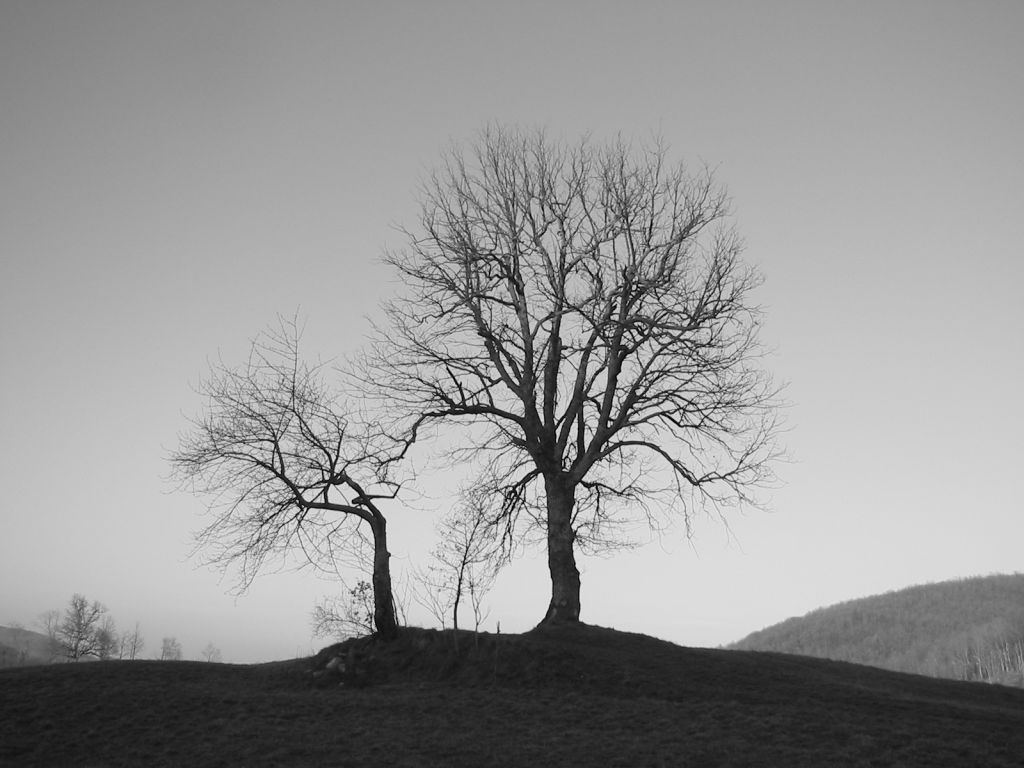
\includegraphics[width=0.4\textwidth]{Ubuntu0}
%\caption{smh}
%\end{wrapfigure}\\

%\section*{Usage}
\noindent{\Large \textbf{Usage Instructions:}}\\
\begin{itemize}
\item This book include all papers I have read from 2017.05.28. \\
\item The {\color{magenta} magenta} represent the online link.\\
\item The {\color[rgb]{1,0,0} red} represents the links in this book including reference, figure, table and others.\\
\item The {\color{purple} purple} represents the emphasize.
\end{itemize}

\nopagebreak

\chapter{Image processing based on CUDA}

This chapter include the Image processing acceleration based on CUDA.

\section{Novel multi-scale retinex with color restoration on graphics processing unit}
\subsection{Abstract}
In this paper, a parallel application of the MSRCR+AL algorithm on a GPU is presented. For the various configurations in our test, the GPU-accelerated MSRCR+AL shows a scalable speedup as the resolution of an image increases. The up to $45 \times$ speed up $(1024 \times 1024)$ over the single-threaded CPU counterpart shows a promissing direction of using the GPU-based MSRCR+AL in large scale, time-critical applications. We also achieved 17 frames per second in video processing $(1280 \times 720)$. 

\subsection{Content}
In our implementation, the CUFFT provides a simple
interface for computing FFTs. After the plans of both
forward and inverse FFTs are created according to the
CUFFT requirements, the image data and the Gaussian
filters can be parallel transformed to frequency domain.
The multiplication between image data and Gaussian filters
in frequency domain is finished by ModulateandNormal-
ize() function, which is also provided by the CUFFT
library.

The atomic function atomicAdd() provided by
CUDA is used in the kernel histogram function to guar-
antee to be performed without interference from other
threads.
\subsection{Parallel optimization strage}
\subsubsection{size of thread block and grid}
For example, the maximum number of
threads on the lower capability version of CUDA is
512, but newer CUDA-enabled GPUs with 2.x computecapability can reach 1,024. But, each streaming multi-
processer (SM) can only execute 1,536 threads simul-
taneously. Therefore, we set the number of threads per
block at 192, which means each SM can fully execute
eight blocks to maximize resources.
\subsubsection{Memory access optimization}
A thread needs 400–600 clock cycles to access the
global memory, but only needs about 4 clock cycles to
access fast memory units such as register and shared
memory due to lower access latency. Therefore, taking
full advantage of the multi-level GPU memory storage
components can obtain quick data access to improve
the execution performance effectively.

\subsubsection{Loop unrolling}
After loop unrolling, the code only needs to run one time to
write the result. The number of write processes decreases
$66.7 \%$ compared with the serial code. Also, it only needs
one time to read the result, compared with three times had
we used in the serial code. The number of read processes
decreases $66.7 \% $ as well. Furthermore, this loop unrolling
strategy can be applied to sum different scale results
together for the Multi-scale Retinex. More importantly, in
the reduction algorithm for the summation process, this
strategy is used to greatly increase the calculation speed
and reduce the instruction overhead.
\subsection{Conclusion}
see the Abstract subsection.

\section{Image Convolution}
This section includes all articles I have read relating to Image Convolution using CUDA.
Image convolution is usually used in image filtering, like gaussian filter.
\subsection{Na\"ive  Implementation}
From the idea of convolutio filter itself, the most naive approach is to use global memory to send data to device and each thread accesses this to compute convolution kernel. Our convolution kernel size is radius 8 (total $17 \times 17$ multiplicaiton for single pixel value). In image border area, reference value will be set to 0 during computation. This naive approach includes many of conditional statements and this causes very slow execution.
\begin{figure}[!hbtp]
\centering
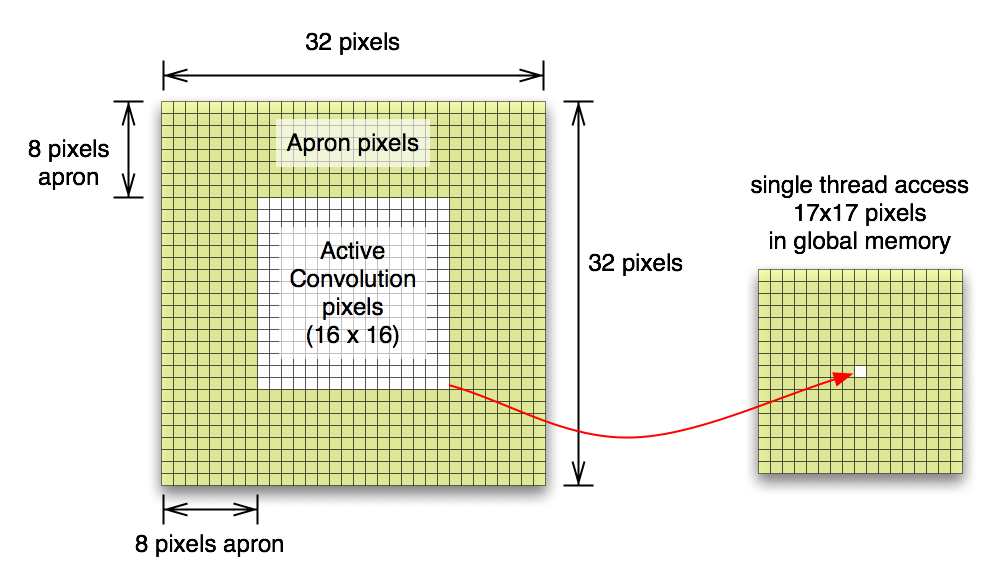
\includegraphics[width=0.8\textwidth]{CUDAImageProcessing/ImageConvoOnGlobal}
\caption{Image Convolution based on Global Memory}
\label{fig3.1}
\end{figure}
The code is as shown below:

\lstdefinestyle{customCpp}{
 belowcaptionskip=1\baselineskip,
  breaklines=true,
%  frame=L,
  xleftmargin=\parindent,
  language=C,
  showstringspaces=false,
  basicstyle=\footnotesize\ttfamily,
  keywordstyle=\bfseries\color{green!40!black},
  commentstyle=\itshape\color{purple!40!black},
  identifierstyle=\color{blue},
  stringstyle=\color{orange},
}

\lstset{style=customCpp,caption={Image Convolution based on global memory}}
\lstinputlisting{CUDAImageProcessing/filterGlobal.cu}

For $396 \star 396$ input image, the time is 1.6ms.
When the input filter is stored in constant memory or specified by {\color{red}{'\_\_restrict\_\_'}}, the time is 1.7 or 1.8 ms.

\subsection{Na\"ive Shared Memory Implementation}
The simplest approach to implement convolution in CUDA is to load a block of the
image into a shared memory array, do a point-wise multiplication of a filter-size portion of
the block, and then write this sum into the output image in device memory. Each thread
block processes one block in the image. Each thread generates a single output pixel.

The algorithm itself is somewhat complex. For any reasonable filter kernel size, the
pixels at the edge of the shared memory array will depend on pixels not in shared memory.
Around the image block within a thread block, there is an \textit{apron} of pixels of the width of the
kernel radius that is required in order to filter the image block. Thus, each thread block
must load into shared memory the pixels to be filtered and the apron pixels.

Note: The apron of one block overlaps with adjacent blocks. The aprons of the
blocks on the edges of the image extend outside the image – these pixels can either be
clamped to the color of pixels at the image edge, or they can be set to zero.

\begin{figure}[!hbtp]
\centering
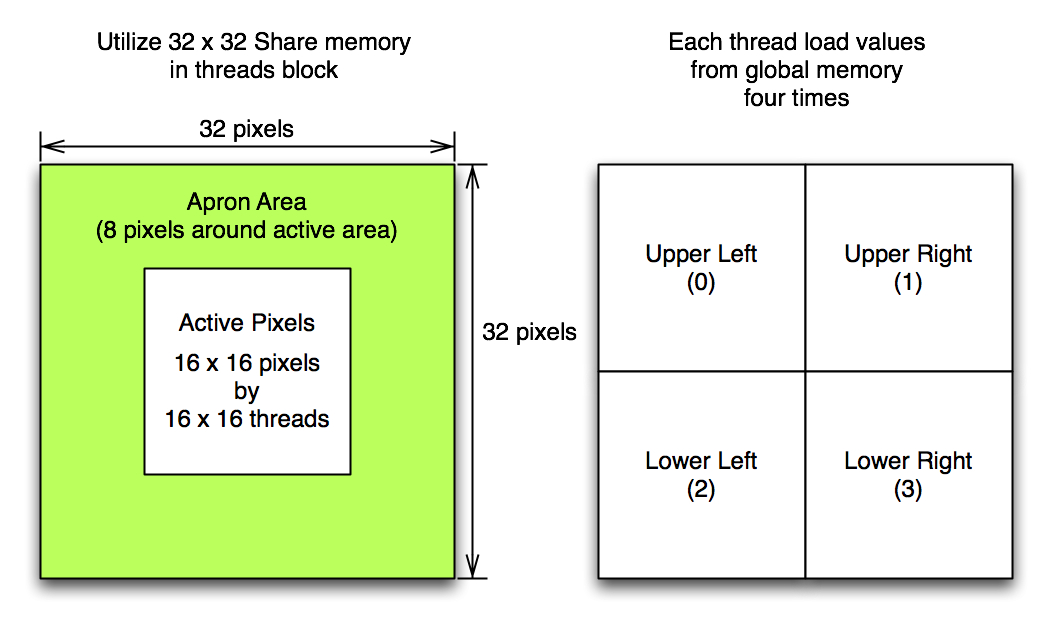
\includegraphics[width=0.9\textwidth]{CUDAImageProcessing/ImageConvoOnShare1}
\caption{Image Convolution based on shared memory}
\label{fig3.2}
\end{figure}

The first attempt was to keep active thread size as same as previous and increase block size for apron pixels. This did not work since convolution kernel radius is 8 and it make block size to $32 \times 32$ (1024). This is bigger than G80 hardware limit (512 threads max per block).

Therefore, I changes scheme as all threads are active and each thread loads four pixels and keep the block size $16 \times 16$. Shared Memory size used is $32 \times 32$ (this includes all necessary apron pixel values for $16 \times 16$ active pixels). Below shows quite a bit of performance improve. This is almost $\times2.8$ speed up over naive approach (in 2048 resolution).

\lstset{style=customCpp, caption={Image colvotion based on Shared memory and Apron}}
\lstinputlisting{CUDAImageProcessing/filterShare.cu}

Note : the value \verb|“gLoc - KERNEL_RADIUS - IMUL(dataW, KERNEL_RADIUS)”| is the shift address of the image data on the upper left corner.
在本方法中,主要是索引的问题,所以又分为Share Memory的索引 以及 图像数据的索引。在具体实现过程中,选择是固定thread Block的大小,同时在share memory中添加边界。所以将图像数据拷贝到Share Memory中时,分了四次,分别对应:左上角,右上角,左下角、右下角。也就是图\ref{fig3.2}中的对应关系,其处理过程就是将小的图像块映射到大的Share memory中,从这个方面进行理解。

\subsection{Separable Gaussian Filtering}
\subsubsection{Separable Convolution}
A tow-dimensional filter s is said to be separable if it can be written as the convolution of tow one-dimesional filters \textit{\textbf{v}} and \textit{\textbf{h}}:
\begin{displaymath}
s = v * h
\end{displaymath}
''How to determine if a matrix is an outer product of two vectors?''\\
''Go look at the \textbf{rank} function. ''.
Of course. If a matrix is an outer product of two vectors, its rank is 1. 

So the test is this: The rank of A is the number of nonzero singular values of A, with some numerical tolerance based on eps and the size of A.

So how can we determine the outer product vectors? The answer is to go back to the svd function. Here's a snippet from the doc:

$[U, S, V] = svd(X)$ produces a diagonal matrix S of the same dimension as X, with nonnegative diagonal elements in decreasing order, and unitary matrices \textit{\textbf{U}} and \textit{\textbf{V}} so that
$X = U * S * V'$

A rank 1 matrix has only one nonzero singular value, so $X = U * S * V'$ becomes $U(:, 1) * S(1, 1) * V(:,1)$. This is basically the outer product we were seeking. Therefore, we want the first columns of \textit{\textbf{U}} and \textit{\textbf{V}}. (We have to remember also to use the nonzero singular value as a scale factor.)

\subsubsection{Seperate Gaussian filter}
First chose, somewhat artitrarily to split the scale factor, S(1, 1), "equally" between \textit{\textbf{v}} and \textit{\textbf{h}}. Except for normal floating-point roundoff differences, gaussian and v*h are equal. Just show as following : 
\begin{displaymath}
\begin{gathered}
\left[ U, S, V \right]= svd(X)\\
v = U(:, 1) * sqrt(S(1, 1))\\
h = V(:, 1)‘ × sqrt(S(1, 1))\\
GassianFilter = v * h
\end{gathered}
\end{displaymath}
More details can be found at :\href{http://blogs.mathworks.com/steve/2006/11/28/separable-convolution-part-2/}{Separable Convolution}.

\subsection{Optimizing for memory coalescence}
Base read/write addresses of the warps of 32 threads also must meet half-warp
alignment requirement in order to be coalesced. If four-byte values are read, then the base
address for the warp must be 64-byte aligned, and threads within the warp must read
sequential 4-byte addresses. If the dataset with apron does not align in this way, then we
must fix it so that it does.

The approach used in the row filter is to have additional threads on the leading edge
of the processing tile, in order to make threadIdx.x == 0 always reading properly aligned
address and thus to meet global memory alignment constraints for all warps. This may seem
like a waste of threads, but it is of little importance when the data block, processed by a
single thread block is large enough, which decreases the ratio of apron pixels to output
pixels.

Each image convolution pass in both row and column pass is separated into two
sub stages within corresponding CUDA kernels. The first stage loads the data from global
memory into shared memory, and the second stage performs the filtering and writes the
results back to global memory. We mustn’t forget about the cases when row or column
processing tile becomes clamped by image borders, and initialize clamped shared memory array indices with correct values. Indices not lying within input image borders are usually
initialized either with zeroes or with values, corresponding to clamped image coordinates. In
this sample we opt for the former.

In between the two stages there is a \textbf{\_\_syncthreads( )} call to ensure that all threads
have written to shared memory before any processing begins. This is necessary because
threads are dependent on data loaded by other threads.

For both the loading and processing stages each active thread loads/outputs one
pixel. In the computation stage each thread loops over a width of twice the filter radius plus
1, multiplying each pixel by the corresponding filter coefficient stored in constant memory.
Each thread in a half-warp accesses the same constant address and hence there is no penalty
due to constant memory bank conflicts. Also, consecutive threads always access consecutive
shared memory addresses so no shared memory bank conflicts occur as well.

The column filter pass operates much like the row filter pass. The major difference
is that thread IDs increase across the filter region rather than along it. As in the row filter
pass, threads in a single half-warp always access different shared memory banks, but the
calculation of the next/previous addresses involves increment/decrement by
COLUMN\_TILE\_W, rather than simply 1. In the column filter pass we do not have inactive
“coalescing alignment” threads during the load stage, because we assume that the tile width
is a multiple of the coalesced read size. In order to decrease the ratio of apron to output
pixels we want image tile to be as tall as possible, so to have reasonable shared memory
utilization we shoot for as thin image tiles as possible: 16 columns.

\section{CUDA C Best Practice Guide}
\subsection{Performance Metrics}
\subsubsection{Timing}
\begin{itemize}
\item Using CPU Timers \\
	Should call \textit{cudaDeviceSynchronize()} immediately before starting and stopping the CPU timer.
\item Using CUDA GPU Timers\\
	The device will record a timestamp for the event when it reaches that event in the stream. This value is expressed in milliseconds and has a resolution of approximately half a microsecond.
\end{itemize}
\subsubsection{Bandwidth}
Bandwidth - the rate at which data can be transferred - is one of the most important gating factors for performance.


\section{Npp Library Image Filters}
\subsection{Image Data}
\subsubsection{Line Step}
All image data passed to NPPI primitives requires a line step to be provided. It is important to keep in mind that this line step is always specified in terms of bytes, not pixels.

\section{PTX ISA 6.0}
\subsection{PTX Machine Model}
The \textit{Multiprocessor} maps each thread to one \textit{scalar processor} core, and each scalar thread executes independently with its own instruction address and register state.

Individual threads composing a SIMT warp start together at the same program address but are otherwise free to branch and execute independently. A warp executes one common instruction at a time, so full efficiency is realized when all threads of a warp agree on their execution path. If threads of a warp diverge via a data-dependent
conditional branch, the warp serially executes each branch path taken, disabling threads that are not on that path, and when all paths complete, the threads converge back to the same execution path. 

Each multiprocessor has \textbf{on-chip memory} of the four following types : 
\begin{itemize}
\item Local 32-bit registers per processor;
\item Shared memory (parallel data cache);
\item Read-only \textit{constant cache} that is shared by all scalar processor cores;
\item Read-only \textit{texture cache} 
\end{itemize}

The local and global memory spaces are read-write regions of \textbf{device memory} and are not cached.

If there are not enough registers or shared memory available per multiprocessor to process at least one block, the kernel will fail to launch.

\subsubsection{Syntax}
PTX programs are a collection of text source modules(files). PTX source modules have an assembly-language style syntax with instruction operation codes and operands. Pseudo-operations specify symbol and addressing management. The \textit{ptxas}
optimizing backend compiler optimizes and assembles PTX source modules to produce
corresponding binary object files.
\subsubsection{Source Format}
PTX is case sensitive and uses lowercase for keywords.

Each PTX module must begin with a \textbf{.version} directive specifying the PTX language version, followed by a \textbf{.target} directive specifying the target architecture assumed. 

\subsubsection{Statements}
A PTX statement is either a \textbf{directive} or an \textbf{instruction}. Statements begin with an optional label and end with a semicolon.
\begin{itemize}
\item Directive Statements \\
Directive keywords begin with a dot, so no conflict is possible with user-defined
identifiers. 如图\ref{PTXDirectives}所示。
\begin{figure}[!htbp]
\centering
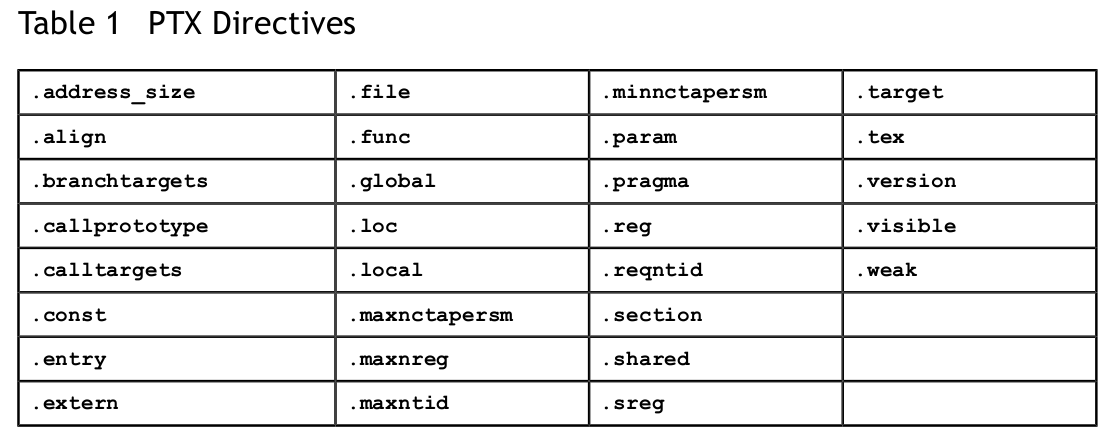
\includegraphics[width=0.9\textwidth]{CUDAImageProcessing/PTXDirectives}
\caption{PTX Directives}
\label{PTXDirectives}
\end{figure}
%\begin{table}[!htbp]
%\begin{tabular}{c|c|c}
%\hline
%A & B & C \\
%\hline
%\end{tabular}
%\end{table}
\item Instruction Statements \\
Instructions are formed from an instruction opcode followed by a \textbf{comma-separated} list
of zero or more operands, and terminated with a semicolon.

Operands may be register
variables, constant expressions, address expressions, or label names.
The guard predicate
follows the optional label and precedes the opcode, and is written as \textbf{@p} , where p is a
predicate register. The guard predicate may be optionally negated, written as \textbf{@!p}.

The destination operand is first, followed by source operands.
如图\ref{ReservedInstructionKeywords}所示。
\begin{figure}[!hbtp]
\centering
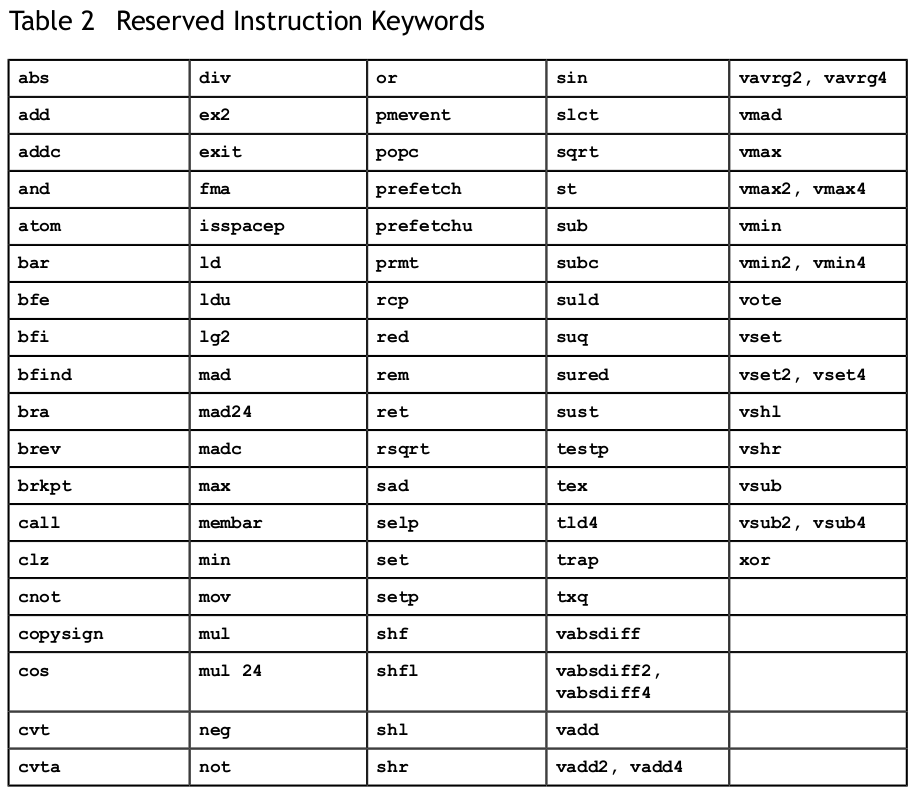
\includegraphics[width=0.9\textwidth]{CUDAImageProcessing/ReservedInstructionKeywords}
\caption{Reserved Instruction Keywords}
\label{ReservedInstructionKeywords}
\end{figure}


\end{itemize}




\chapter{FPGAs}
{
\large
Every section is arranged like follows:
\begin{itemize}
\item Abstract\\
	The abstract part of paper.
\item Content\\
	The main idea of paper.
\item Results\\
	The experiment implementation.
\item Conclusion \\
	The conclusion part of paper.
\end{itemize}
}
\section{Performance Comparison of FPGA, GPU and CPU in Image Processing 2009}
%\noindent {\Large \textbf{Abstract}}\\
\subsection{Abstract}
\indent \textbf{Many applications in image processing have high inherent
parallelism}. FPGAs have shown very high performance in
spite of their low operational frequency by fully extracting
the parallelism. In recent micro processors, it also becomes
possible to utilize the parallelism using multi-cores which
support improved SIMD instructions, though programmers
have to use them explicitly to achieve high performance. Re-
cent GPUs support a large number of cores, and have a po-
tential for high performance in many applications. \textbf{However,
the cores are grouped, and data transfer between the groups
is very limited.} Programming tools for FPGA, SIMD in-
structions on CPU and a large number of cores on GPU have
been developed, but it is still difficult to achieve high perfor-
mance on these platforms. In this paper, we compare the per-
formance of FPGA, GPU and CPU using three applications
in image processing; two-dimensional filters, stereo-vision
and k-means clustering, and make it clear which platform is
faster under which conditions.

\begin{figure*}[t]
\centering
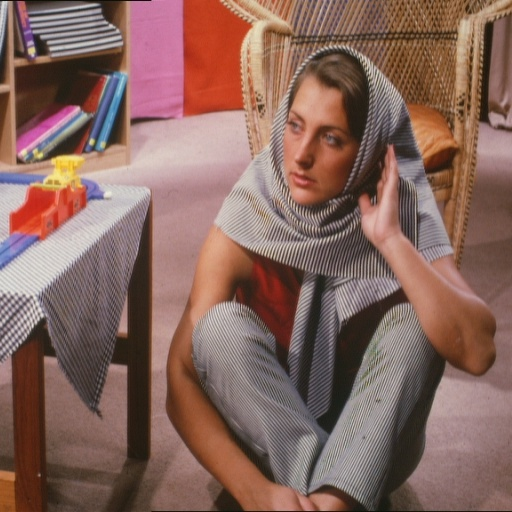
\includegraphics[width=0.9\textwidth]{Barbara.jpg}
\caption{传统提升小波计算过程}
\label{figWavelet}
\end{figure*}


\subsection{Content}
Compared three applications: two-dimension filters, stereo-vision, k-means clustering.\\

The high performance of FPGA comes from its flexibility which makes it possible to realize the fully optimized circuit for each application, and a large number of on-chip memory banks which supports the high parallelism.{\bfseries FPGA can achieve extremely high
performance in many applications in spite of its low op-
erational frequency}.\\

GPU cores are grouped, the data transfer between groups is very slow. \\

\noindent\textbf{GPU Analysis}\\
\indent It consists of 10 thread processor clus-
ters. A thread processor cluster has three streaming mul-
tiprocessors, eight texture filtering units, and one level-1
cache memory. Each streaming multiprocessor has one in-
struction unit, eight stream processors (SPs) and one local
memory (16KB). Thus, GTX280 has 240 SPs in total. Eight
SPs in a streaming multiprocessor are connected to one in-
struction unit. This means that the eight SPs execute the
same instruction stream on different data.

\noindent \textbf{Two-Dimensional Filters}\\
\indent The computational complexity of filters is $O(w \times w)$, and $w$ is radius of filter.
\begin{figure}[!hbtp]
\centering
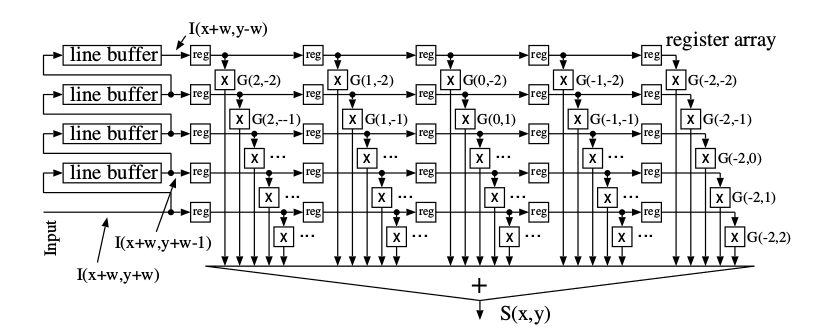
\includegraphics[width=0.9\textwidth]{FPGAs/Paper1_1_Cirsuitsfornon-separablefilters}
\caption{Circuits for non-separable filters}
\label{fig1.1}
\end{figure}\\
Fig\ref{fig1.1} shows the filter is $5 \times 5$ case.\\
\noindent \textbf{Stereo Vision}\\
\indent This application is to get the distance to the location obtained from the two camera's disparity.The sum of absolute difference (SAD) is widely used to compared the windows because of its simplicity\index{SAD}. 
More details can be found in paper\cite{asano2009performance}.
\noindent\textbf{K-means Clustering}\\
\indent More details can be found in paper \cite{asano2009performance}.
\subsection{Results}
\begin{itemize}
\item Xilinx XC4VLX160.
\item GeForce 280GTX, 1 GB DDR3, CUDA version 2.1.
\item Intel Core2 Extreme QX6859.
\end{itemize}
The time to download images from main memory is not included. CPU has four cores, FPGA is fixed to 100MHz. Fig is the performance of two-dimension filters.
\begin{figure}[!hbtp]
\centering
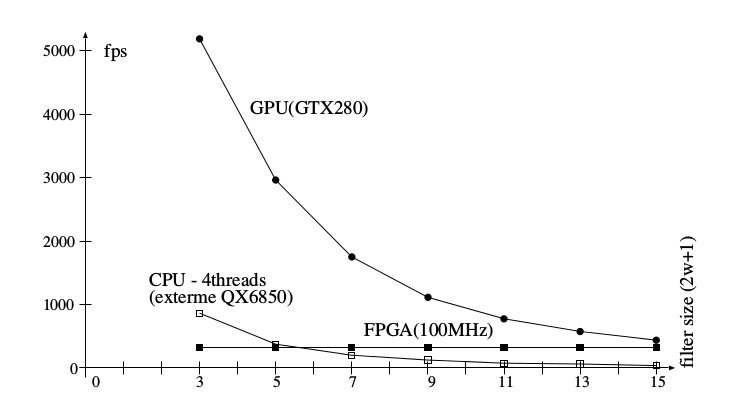
\includegraphics[width=0.9\textwidth]{FPGAs/Paper1_1_PerformanceofTwo-DimensionFilters}
\caption{Performance of two-dimensional filters}
\label{fig1.2}
\end{figure}\\
\indent GPU is the fastest for all tested filter size.In this
problem, filters can be applied to each pixel in the image in-
dependently without using shared variables. So, GPU can
show its best performance.\\

{\color{purple} In the later two applications, the performance FPGA is much better than GPU.}
\subsection{Conclusion}
\indent We have compared the performance of GPU with FPGA
and CPU (quad-cores) using three simple problems in im-
age processing. GPU has a potential for achieving almost
the same performance with FPGA. The number of cores in
GTX280 is 240.Considering the trade-offs between the operational frequency of GPU (more than 10 times faster), and
the fine-grained parallelism in FPGA, this seems to be a
natural consequence. However, GPU can show its potential
only for naive computation methods, in which all pixels can
be processed independently. For more sophisticated algorithms  
which use shared arrays, GPU can not execute those
algorithms because of its very small local memory, or can
not show good performance because of the memory access
limitation caused by its memory architecture. GPU is slower
than CPU in those algorithms (it may be possible to realize
much better performance if we can find algorithms which
can get around the limitations, but we could not find them).
The performance of CPU is 1/12 - 1/7 of FPGA, which
means that CPU with quad-cores can executes about 1/10
operations of FPGA in a unit time (the same algorithms are
executed on CPU and FPGA). The performance of FPGA
is limited by the size of FPGA and the memory bandwidth.
With a latest FPGA board with DDR-II DRAM and a larger
FPGA, it possible to double the performance by processing
twice the number of pixels in parallel.\\
\indent We have the following issues which have to be consid-
ered. We have compared the performance using only three
problems. The performances of the programs on GPU and
CPU are not fully tuned up. In the comparison, power con-
sumption and costs are not considered.

\section{Fast FPGA Prototyping for real-time image processing with very high-level synthesis 2017}
\subsection{Abstract}
Programming in high abstraction level can facilitate the development of digital signal processing systems. In the recent 20 yeahs, HLS has made significantly progress. However, due to the high complexity and computational intensity, image processing algorithms usually necessitate a higher abstraction environment than C-synthesis, and the current HLS tools do not have the ability of this kind. This paper presents a conception of very high-level synthesis method which allows fast prototyping and verifying the FPGA-based image processing designs in the MATLAB environment. We build a heterogeneous development flow by using currently available tool kits for verifying the proposed approach and evaluated it within two real-life applications. Experiment results demonstrate that it can effectively reduce the complexity of the development by automatically synthesizing the algorithm behavior from the user level into the low register transfer level and give play to the advantages of FPGA related to the other devices.
\subsection{Content}
Advanced Digital Sciences Center(ADSC) of the University of Illinois reported that FPGA can achieve a speedup to 2-2.5x and save 84-92\% of the energy consumption comparing to Graphics Processing Units(GPUs). ADSC indicates also that a manual FPGA design may consume 6-18 months and even years for a full custom hardware, while the GPUs(CUDA) based designed only 1-2 weeks. \\

Fig\ref{fig1.3} show the Gasjki-Kuhn's Y-chart comparing the conventional RTL with the HLS-based design flows.\\
\begin{figure}[!hbtp]
\centering
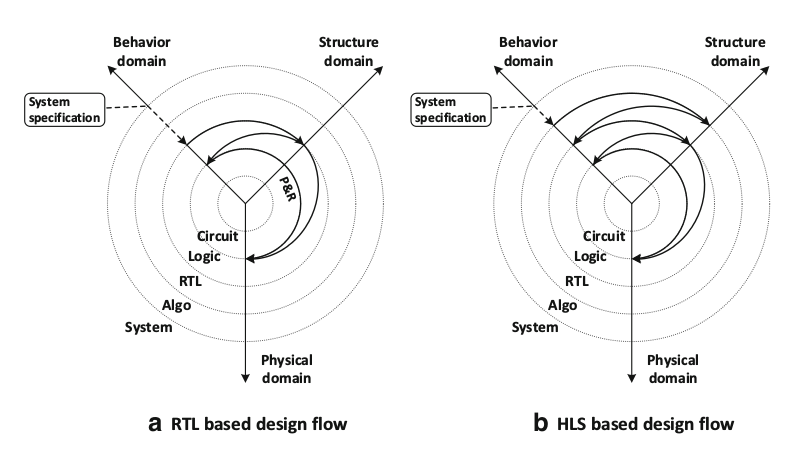
\includegraphics[width=0.9\textwidth]{FPGAs/Paper1_2_Comparison}
\caption{Comparison of RTL- and HLS-based design flows by using Gasjki-Kuhn's Y-chart: full lines indicate the automated cycles, while dotted lines the manual cycles.}
\label{fig1.3}
\end{figure}
The challenges of MATLAB-to-RTL synthesis include:
\begin{itemize}
\item Operators in MATLAB perform different operations depending on the type of the operands, whereas the functions of the operators in RTL are fixed.
\item MATLAB includes very simple and powerful vector operations such as the concatenation ``[ ]'' and column operators ``$x(:)$'' or ``end'' construct, which can be quite hard to map to RTL.
\item MATLAB supports ``polymorphism'' whereas RTL does not. More precisely, functions in MATLAB are genetic and can process different types of input parameters. In the behaviors of RTL, each parameter has only a single given type, which cannot change.
\item MATLAB supports dynamic loop bounds or vector size, whereas RTL requires users to initialize explicitly them and cannot do any changes during the synthesis.
\item The variables in MATLAB can be reused for different contents (different types), whereas RTL does not, as each variable has one unique type.
\end{itemize}
\par\indent Two complex image processing applications: Kubelka-Munk genetic algorithm(KMGA) for the multispectral image based skin lesion assessments \& level set method(LSM)-based algorithm for very high-resolution(VHR) satellite image segmentation.\index{KMGA}\index{LSM}\index{VHR}.

\chapter{Image Fusion}
\section{Guided Image Filter 2013}
\subsection{Abstract}
In this paper, we propose a novel explicit image filter called guided filter. Derived from a local linear model, the guided filter
computes the filtering output by considering the content of a guidance image, which can be the input image itself or another different
image. The guided filter can be used as an edge-preserving smoothing operator like the popular bilateral filter, but it has better
behaviors near edges. The guided filter is also a more generic concept beyond smoothing: It can transfer the structures of the guidance
image to the filtering output, enabling new filtering applications like dehazing and guided feathering. Moreover, the guided filter
naturally has a fast and nonapproximate linear time algorithm, regardless of the kernel size and the intensity range. Currently, it is one
of the fastest edge-preserving filters. Experiments show that the guided filter is both effective and efficient in a great variety of
computer vision and computer graphics applications, including edge-aware smoothing, detail enhancement, HDR compression, image
matting/feathering, dehazing, joint upsampling, etc.
\subsection{Content}
A general linear translation-variant filtering process, which involves a guidance image \textit{I}, an filtering input image \textit{p} and an output image \textit{q}. Both \textit{I} and \textit{p} are given beforehand according to the application, and they can be \textbf{identical}! The filtering output at a pixel \textit{i} is expressed as a weight average:
\begin{equation}
\centering
q_i = \sum_{j}W_{ij}(I)p_j
\end{equation}
where \textit{i, j} are pixel indexes. The filter kernel \(W_{ij}\) is a function of the guidance image \textit{I} and independent of \textit{p}.
\subsection{Conclusion}

\section{Multiscale Image Fusion Through Guided Filtering}
\subsection{Abstract}
We introduce a multiscale image fusion scheme based on GUided Filtering. Guided filtering can effectively reduce noise while preserving details boundaries. While  restoring larger scale edges. The proposed multi-scale fusion scheme achieves optimal spatial consistency by using guided filtering both at the decomposing and at the recombination stage of the multiscale fusion process. First, size-selective iterative guided filtering is applied to decompose the source images into base and detail layers at multiple levels of resolution. Next, at each resolution level a binary weighting map is obtained as the pixelwise maximum of
corresponding source saliency maps. Guided filtering of the binary weighting maps with their corresponding source images as guidance images serves to reduce noise and to restore spatial consistency. The final fused image is obtained as the weighted recombination of the individual detail layers and the mean of the lowest resolution base layers. Application to multiband visual (intensified) and thermal infrared imagery demonstrates that the proposed method obtains state-of-the-art performance for the fusion of multispectral nightvision images. The method has a simple implementation and is computationally efficient\cite{toet2016multiscale}.

\subsection{Contents}
To data, a variety of image fusion algorithms have been proposed. A popular class of algorithms are the multi-scale image fusion schemes, which decompose the source images into spatial primitives at multiple spatial scales, then integrate these primitives to form a new multi-scale transform-based representation, and finally apply an inverse multi-scale transform to reconstruct the fused image. However, most of these techniques are computationally expensive and tend to oversharpen edges, which makes them less suitable for application in multiscale schemes

Bilateral Filter: It can reverse the intensity gradient near sharp edges.

Guided Filter: 

The two filtering conditions are:
\begin{itemize}
\item the local filter output is a linear transform of the guidance image \textit{G}
\item as similar as possible to the input image \textit{I}.
\end{itemize}
The first condition implies that:
\begin{displaymath}
O_i = a_kG_i + b_k \qquad \forall i \in \omega_k
\end{displaymath}
where the $\omega_k$ is a square window of size $(2r + 1) \times (2r+1)$. {\bfseries The local linear model ensures that the output image $O$ has an edge only at locations where the guidance image $G$ also has one.} Linear coefficients $a_k$ and $b_k$ are constant in $\omega_k$. They can be estimated by minimizing the squared difference between the output image $O$ and the input image $I$ in the window $\omega_k$, i.e. minimizing the cost function $E$:
\begin{displaymath}
E(a_k, b_k) = \sum_{i \in \omega_k}\left((a_kG_i + b_k - I_i)^2 + \epsilon a_k^2 \right)
\end{displaymath}
where $\epsilon_k$ is a regularization parameter penalizing large $a_k$. The coefficients $a_k$ and $b_k$ can directly be solved by linear regression. Since pixel $i$ is contained in several different window $\omega_k$, the value of $O_i$ depends on the window over which it is calculated:
\begin{displaymath}
O_I = \overline{a}_i G_i + \overline{b}_i
\end{displaymath}
The abrupt intensity changes in the guiding image $G$ are still largely preserved in the output image $O$. The guided filter is a computationally efficient, edge-preserving operator which avoids the gradient reversal artefacts of the bilateral filter. 

In Iterative guided filtering: In such a scheme the result $G^{t+1}$ of the t-\textit{th} iteration is obtained from the joint bilateral filtering of the input image $I$ using the result $G^t$ of the previous iteration step:
\begin{displaymath}
G^{t+1}_i = \frac{1}{K_i}\sum_{j \in \omega}I_j \cdot f(\parallel i - j \parallel) \cdot g(\parallel G^t_i - G^t_j \parallel )
\end{displaymath}
Note that the initial guidance image $G^1$ can simply be a constant (e.g. zero) valued image since it updates to the Gaussian filtered input image in the first iteration step.

Proposed Method:
\begin{itemize}
\item Iterative guided filtering is applied to decompose the source images into base layers (representing large scale variations) and detail layers (containing small scale variations).
\item Frequency-tuned filtering is used to generate saliency maps for the source images.
\item Binary weighting maps are computed as the pixelwise maximum of the individual source saliency maps.
\item Guided filtering is applied to each binary weighting map with its corresponding source as the guidance image to reduce noise and to restore spatial consistency.
\item The fused image is computed as a weighted recombination of the individual source detail layers.
\end{itemize}

\textbf{Visual saliency} refers to the physical, bottom-up distinctness of image details. It is a relative property that depends on the degree to which a detail is visually distinct from its background. {\bfseries \color{red} Since saliency quantifies the relative visual importance of image details saliency maps are frequently used in the weighted recombination phase of multiscale image fusion schemes}. Frequency tuned filtering computes bottom-up saliency as local multiscale luminance contrast. The saliency map S for an image I is computed as 
\begin{displaymath}
S(x, y) = \parallel I_\mu - I_f(x,y) \parallel 
\end{displaymath}
where\\
\indent $I_\mu$ is the arithmetic mean image feature vector\\
\indent $I_f$ represents a Gaussian blurred version of the original image, using a 5 * 5 separable binomial kernel\\
\indent $\parallel \cdot \parallel $ is the $L_2$ norm(Euclidian distance), and x, y are the pixel coordinates.\\
\indent We compute saliency using frequency tuned filtering since a recent and extensive evaluation study comparing 13 state-of-the-art saliency models found that the output of this simple saliency model correlates more strongly with human visual perception than the output produced by any of the other available models.

Binary weight maps $BW_{X_i}$ and $BW_{Y_i}$ are then computed by taking the pixelwise maximum of corresponding saliency maps $S_{X_i}$ and $S_{Y_i}$:

\begin{gather*}
BW_{X_i}(x, y) =    
\begin{cases}
1 & \mathrm{if} \: S_{X_i}(x, y) > S_{Y_i}(x, y) \\
0 & \mathrm{otherwise}
\end{cases}\\
BW_{Y_i}(x,y) = 
\begin{cases}
1 & \mathrm{if} \: S_{Y_i}(x, y) > S_{X_i}(x, y)\\
0 & \mathrm{otherwise}
\end{cases}
\end{gather*}
The resulting binary weight maps are noisy and typically not well aligned with object boundaries, which may give rise to artefacts in the final fused image. Spatial consistency is therefore restored through guided filtering (GF) of these binary
weight maps with the corresponding source layers as guidance images
\begin{gather*}
W_{X_i} = GF(BW_{X_i}, X_i) \\
W_{Y_i} = GF(BW_{Y_i}, Y_i)
\end{gather*}

Fused detail layers are then computed as the normalized weighted mean of the corresponding source detail layers:
\begin{displaymath}
dF_i = \frac{W_{X_i} \cdot dX_i + W_{Y_i} \cdot dY_i}{W_{X_i} + W_{Y_i}}
\end{displaymath}

The fused image $F$ is finally obtained by adding the fused detail layers to the average value of the lowest resolution source layers:
\begin{displaymath}
F = \frac{X_3 + Y_3}{2} + \sum_{i=0}^{2}dF_i
\end{displaymath}

By using guided filtering both in the decomposition stage and in the recombination stage, this proposed fusion scheme optimally benefits from both the multi-scale edge-preserving characteristics (in the iterative framework) and the structure
restoring capabilities (through guidance by the original source images) of the guided filter. The method is easy to implement and computationally efficient.

\subsection{Conclusion}
We propose a multiscale image fusion scheme based on guided filtering. Iterative guided filtering is used to decompose the source images into base and detail layers. Initial binary weighting maps are computed as the pixelwise maximum of
the individual source saliency maps, obtained from frequency tuned filtering. Spatially consistent and smooth weighting maps are then obtained through guided filtering of the binary weighting maps with their corresponding source layers as
guidance images. Saliency weighted recombination of the individual source detail layers and the mean of the lowest resolution source layers finally yields the fused image. The proposed multi-scale image fusion scheme achieves spatial consistency by using guided filtering both at the decomposition and at the recombination stage of the multiscale fusion process. Application to multiband visual (intensified) and thermal infrared imagery demonstrates that the proposed method obtains state-of-the-art performance for the fusion of multispectral nightvision images. The method has a simple implementation and is computationally efficient.

\section{Image Fusion With Guided Filtering}
\subsection{Abstract}
A fast and effective image fusion method is proposed for creating a highly informative fused image through merging multiple images. The proposed method is based on a two-scale decomposition of an image into a base layer containing large scale variations in intensity, and a detail layer capturing small scale details. A novel guided filtering-based weighted average technique is proposed to make full use of spatial consistency for fusion of the base and detail layers. Experimental results
demonstrate that the proposed method can obtain state-of-the-art performance for fusion of multispectral, multifocus, multimodal, and multiexposure images.
\subsection{Contents}
\subsubsection{Guided Filter}
The filtering output $O$ is linear transformation of the guidance image $I$ in a local window $\omega_k$ centered at pixel $k$:
\begin{displaymath}
O_i = a_k I_i + b_k \qquad \forall i \in \omega_k
\end{displaymath}
where $\omega_k$ is a square window of size $(2r+1) \times (2r+1)$. The linear coefficients $a_k$ and $b_k$ are contant in $\omega_k$ by minimizing the squared difference between the output image $O$ and the input iamge $P$:
\begin{displaymath}
E(a_k, b_k) = \sum_{i \in \omega_k}\left( (a_kI_i + b_k - P_i) + \epsilon a_k^2 \right)
\end{displaymath}
where $\epsilon$ is a regularization parameter given by the user.
The coefficients can be directly solved by linear regression as follows:
\begin{gather*}
a_k = \frac{\frac{1}{|\omega|}\sum_{i \in \omega_k}I_iP_i -  \mu_k \overline{P}_k}{\delta_k + \epsilon}
\\
b_k = \overline{P}_k - a_k \mu_k
\end{gather*}
where $\mu_k$ and $\delta_k$ are the mean and variance of $I$ in $\omega_k$ respectively. $|\omega|$ is the number of pixels in $\omega_k$, and $\overline{P}_k$ is the mean of $P$ in $\omega_k$. Then the output image can be calculated according to above equation.
\begin{displaymath}
O_i = \overline{a}_iI_i + \overline{b}_i
\end{displaymath}
where \(\overline{a}_i = \frac{1}{|\omega|}\sum_{k \in \omega_i}a_k, \overline{b}_i = \frac{1}{|\omega|}\sum_{k \in \omega_i}b_k \). 

The color image situation, the $a_i$ and other calculators become vector version. See \cite{li2013image}.

\subsection{Fusion Frame}
See figure \ref{fig2.1}.
\begin{figure}[!hbpt]
\centering
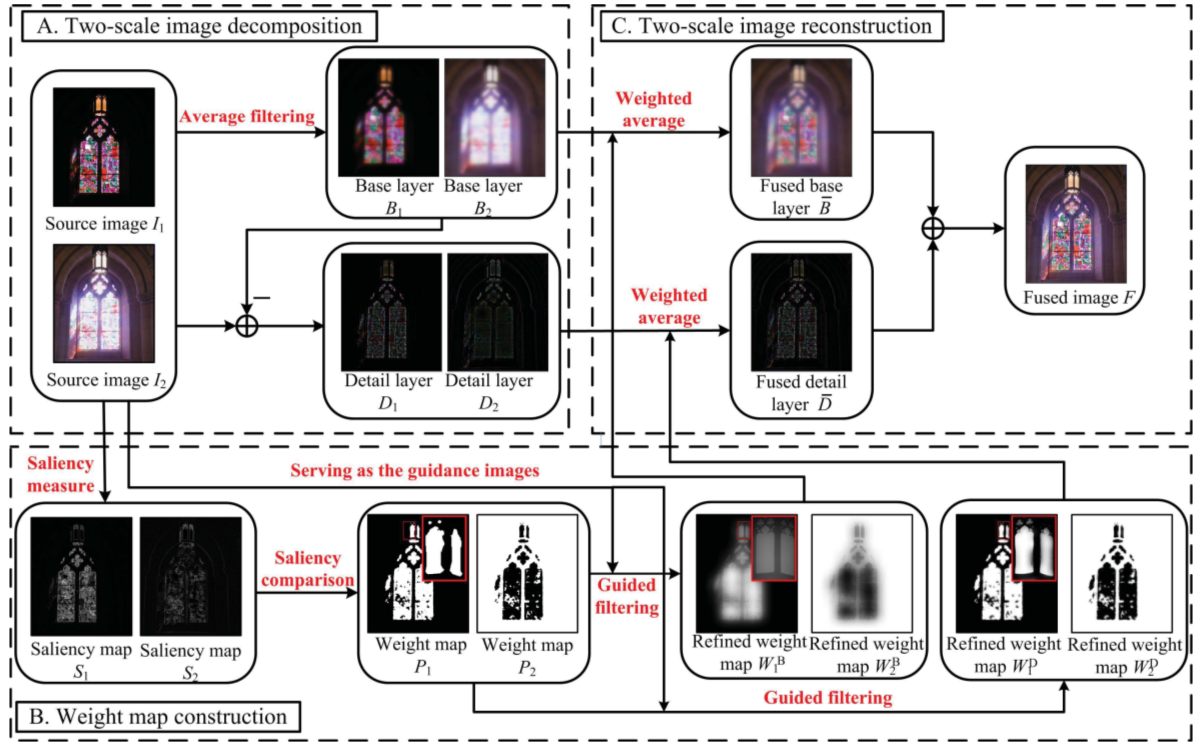
\includegraphics[width=0.9\textwidth]{ImageFusion/ImageFusionGuidedFilter1}
\caption{Schematic diagram of the proposed image fusion method based on guided filtering.}
\label{fig2.1}
\end{figure}

\subsection{Conclusion}

\chapter{Saliency Detection}
This chapter includes papers about saliency detection.
\section{Frequency-tuned Salient Region Detection}
\subsection{Abstract}
In this paper, we introduce a method for salient region detection that outputs full resolution saliency maps with well-defined boundaries of salient
objects. These boundaries are preserved by retaining substantially more frequency content from the original image than other existing techniques. Our method exploits fea-
tures of color and luminance, is simple to implement, and is computationally efficient. We compare our algorithm to five
state-of-the-art salient region detection methods with a frequency domain analysis, ground truth, and a salient object segmentation application. Our method outperforms the five algorithms both on the ground-truth evaluation and on the segmentation task by achieving both higher precision and better recall.
\subsection{Contents}
\subsubsection{Related work}
Saliency estimation methods can broadly be classified as:
\begin{itemize}
\item biologically based
\item purely computational 
\item combination of above two approaches
\end{itemize}

Itti base their method on the biologically plausible architecture proposed by Koch and Ullman. They determine center-surround contrast using a \textbf{Difference of Gaussians}
(DoG)\index{DoG}. Frintrop presetn a method inspired by Itti's method, but they compute \textbf{center-surround differences} with square filters and use integral images to speed up the calculations.

Other methods are purely computational 
and are not based on biological vision principles. Ma and
Zhang  and Achanta et al. estimate saliency us-
ing center-surround feature distances. Hu et al.  es-
timate saliency by applying heuristic measures on initial
saliency measures obtained by histogram thresholding of
feature maps. Gao and Vasconcelos maximize the mu-
tual information between the feature distributions of center
and surround regions in an image, while Hou and Zhang
 rely on frequency domain processing.
 
The third category of methods are those that incorporate
ideas that are partly based on biological models and partly
on computational ones. For instance, Harel et al. create
feature maps using Itti’s method but perform their normal-
ization using a graph based approach. Other methods use
a computational approach like maximization of information
 that represents a biologically plausible model of saliency
detection.
\subsubsection*{Limitations}
The saliency maps generated by most methods have low resolutioni. Itti's method produces saliency maps that are just $1/{256^{th}}$

\subsubsection*{Frequency-tuned Saliency Detection}
\textbf{DoG}

DoG : Difference of Gaussians.  DoG filter is widely used in edge detecion since it closely and efficiently approximates the Laplacian of Gaussian (LoG) filter, cited as the most satisfactory operator for detecting intensity changes when the standard deviations of the Gaussians are in the ratio 1 : 1.6. The DoG has also been used for interest point detection and  saliency detection.  The DoG filter is given by : 
\begin{equation}
\begin{gathered}
DoG(x, y) = \frac{1}{2\pi}\left[
\frac{1}{\delta_1^2}e^{-\frac{x^2 + y^2}{2\delta_1^2}} - 
\frac{1}{\delta_2^2}e^{-\frac{x^2 + y^2}{2\delta_2^2}}
\right]\\
= G(x, y, \delta_1) - G(x, y, \delta_2)
\end{gathered}
\end{equation}
where $\delta_1$ and $\delta_2$ are the standard deviatioins of the Gaussian $(\delta_1 > \delta_2)$.

A DoG filter is a simple band-pass filter whose passband
width is controlled by the ratio $\delta_1 : \delta_2$. 
\subsection{Conclusion}


\chapter{Semantic SLAM}

\section{DeLS-3D: Deep Localization and Segmentation with a 2D Semantic Map\cite{WangWang2018DeLS}}

\subsection{Abstract}

Sensor fusion scheme: Integrates camera videos, Motion sensors (GPS/IMU), and a 3D semantic map.

步骤:
\begin{itemize}
\item Initial Coarse camera pose obtained from consumer-grade GPS/IMU
\item A label map can be rendered from the 3D semantic map.
\item Rendered label map and the RGB image are jointly fed into a pose CNN, yielding a corrected camera pose.
\item A multi-layer RNN is further deployed improve the pose accuracy
\item Based on pose from RNN, a new label map is rendered
\item New label map and the RGB image is fed into a segment CNN which produces per-pixel sematnic label.
\end{itemize}

从结果可以看出,Scene Parsing以及姿态估计两者可以相互改善,从而提高系统的鲁棒性以及精确度。

\subsection{Introduction}

在Localization中,传统的做法是基于特征匹配来做,但这样的坏处是,如果纹理信息较少,那么系统就不稳定,会出错。一种改进办法是利用深度神经网络提取特征。实际道路中包含大量的相似场景以及重复结构,所以前者实用性较差。

在Scene Parsing中,深度神经网络用的很多,最好的基于(FCN + ResNet)的途径。在视频中,可以借助光流信息来提高计算速度以及时间连续性。对于静态场景,可以借助SfM技术来联合Parse以及Reconstruction.但这些方法十分耗时。

相机的姿态信息可以帮助3D语义地图与2D标签地图之间的像素对应。反过来,场景语义又会帮助姿态估计。

\subsection{Framework}

总的工作流程,如图\ref{DeLSFramework}所示:
\begin{figure}
\centering
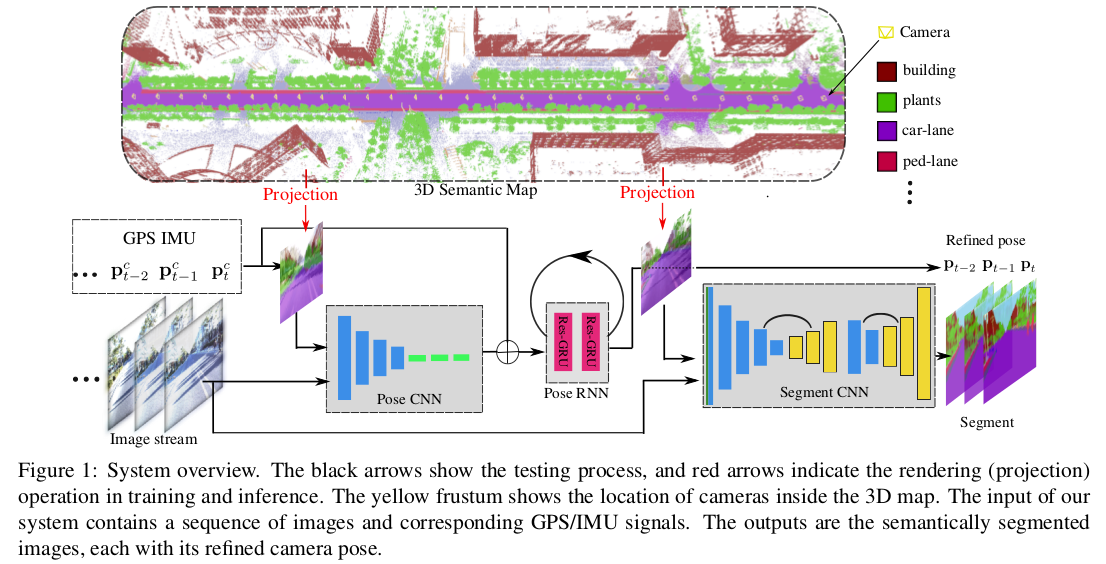
\includegraphics[width=0.95\textwidth]{SemanticSLAM/DeLS1.png}
\caption{DeLS Framwork}
\label{DeLSFramework}
\end{figure}

从图中可以看出,RGB Images 以及 根据GPS/IMU获得的semantic label map被输入到Pose CNN,然后输出的Pose信息输入到Pose RNN来对Pose进一步提高,{\bfseries 这里用RNN来获得前后帧的一致性}!然后在利用新得到的Pose来获取更精确的Semantic Label Map,最后,这个label Map以及RGB图像输入到Segment CNN来进一步提高语义地图的精度。这里标签地图被用于提高语义地图的空间精度以及时间一致性。

网络的训练是基于非常精确地相机姿态以及语义分割,所以可以采用监督学习。

\subsection{Related Work}

\begin{itemize}
\item Camera Pose Estimation

\begin{itemize}
\item PnP

在大的范围内,可能需要提供姿态的先验信息。但对于城市环境中存在大量的Points,这种方法不适用,且不适用于纹理少、结构重复、以及重叠的区域。

\item Deep learned features

PoseNet, LSTM-PoseNet, Bi-Directional LSTM, or Kalman filter LSTM.但实际中由于存在植被等重复性的场景,所以十分有必要加入GPS/IMU等信息来获得鲁棒的定位结果。而在这里,我们采用结合RGB图像与Online Rendered label map的方式来提供更好的结果。

{\bfseries \color{red} 这里问题来了,首先是label map的精度如何?其次,随着时间的变化,label map与实际RGB图像可能完全不同,如季节改变了,这应该如何?}

\end{itemize}

\item Scene Parsing

FCN, Multi-scale context module with dilated convolution, Pooling, CRF, or Spatial RNN with hundreds of layers.这些方法都太耗时了。

一些方法是利用小模型或者模型压缩来加速,但会降低精度。

当输入是Video时,需要考虑时空信息。当前,存在利用光流来帮助label以及semantic在相邻帧之间的传递。借助3D信息以及相机姿态把相邻帧联系起来,可以更好的处理静态背景下的表示。具体的,是使用DeMoN来提高推理效率。

\item Joint 2D-3D for video parsing

CNN-SLAM把传统的3D重建模块替换为深度预测网络,且借助语义分割网络来获取场景语义。同样比较耗时、仅适合静态背景,重建效果也不好。

\end{itemize}

\subsection{Dataset}

\begin{itemize}
\item Data collection

Mobile LIDAR to collect point clouds of the static 3D map. Cameras' resolution: 2018 * 2432.

\item 2D and 3D Labeling

\begin{itemize}
\item Over-segment the point clouds into point clusters based on spatial distances and normal directions, then label each point cluster manually.

\item Prune out the points of static background, label the remaining points of the objects.

\item After 3D-2D projection, only moving object remain unlabeled.

\end{itemize}

\item 使用图形学中的 \textit{Splatting techniques} 来优化未被标签的像素。

\end{itemize}

\subsection{Localizing camera and Scene Parsing}

\subsubsection{Render a label map from a camera pose}

初始的相机的姿态来自于GPS/IMU等传感器。

6-DOF相机姿态:$\mathbf{b} = [\mathbf{q}, \mathbf{t}] \in SE(3)$. 其中$\mathbf{q} \in SO(3)$是四元数表示的旋转,$\mathbf{t} \in \mathbb{R}^3$表示Translation。

在由Point经Spaltting获取其面时,面积大小$s_c$根据Point所属的类别来决定,且与该类别与相机的平均距离的比例有关。

\begin{displaymath}
s_c \propto \frac{1}{|\mathcal{P}_c|}\sum_{x \in \mathcal{P}_c}\min_{\mathbf{t}\in \tau}d(x, t)
\end{displaymath}

其中,$P_c$是属于类别$c$的3D点云,$\tau$是精确地相机姿态。如果面积过大,则会出现Dilated edges,而如果面积过小,则会形成Holes。

\subsubsection{Camera Localization rectification with road prior}

\textbf{CNN-GRU pose Network Architecture}

文中的Pose Network包含一个Pose CNN以及一个Pose GRU-RNN。其中Pose CNN的输入是RGB图像I以及一个标签地图L。输出是一个7维的向量,表示输入图像I与输入标签地图L(由较粗糙的姿态$\mathbf{p}_i^c$得到)之间的位姿关系,从而得到一个在3D Map中更精确的姿态:
$\mathbf{P}_i = \mathbf{p}_i^c + \hat{\mathbf{p}}_i$。

CNN结构借鉴DeMoN,利用打的Kernel Size来获取更大的内容,同时保证运行效率,减少参数量。

由于输入的是图像流,为了保证时间一致性,所以在Pose CNN之后又加上一个多层的GRU网络,且该网络具有Residual Connection的连接结构。结果表明,RNN相比于卡尔曼滤波可以获得更好的运动估计。

\textbf{Pose Loss}

类似于PoseNet的选择,使用Geometric Matching Loss来训练。

\subsubsection{Video Parsing with Pose Guidance}

上一步得到的Pose估计,不是完美的,因为存在light poles存在。由于反光,很多点消失了。此外,由于存在动态物体,这些物体可能在原来的标签地图中不存在,所以这些区域可能发生错误。因此,利用额外的一个Segment CNN来出来这些问题。且利用标签地图来指导分割过程。

\textbf{Segment Network Architecture}

首先基于RGB图像对该网络训练,然后加入标签地图数据进行微调(Fine Tune).具体结构如图\ref{SegmentDeLS}所示。

\begin{figure}[!hbtp]
\centering
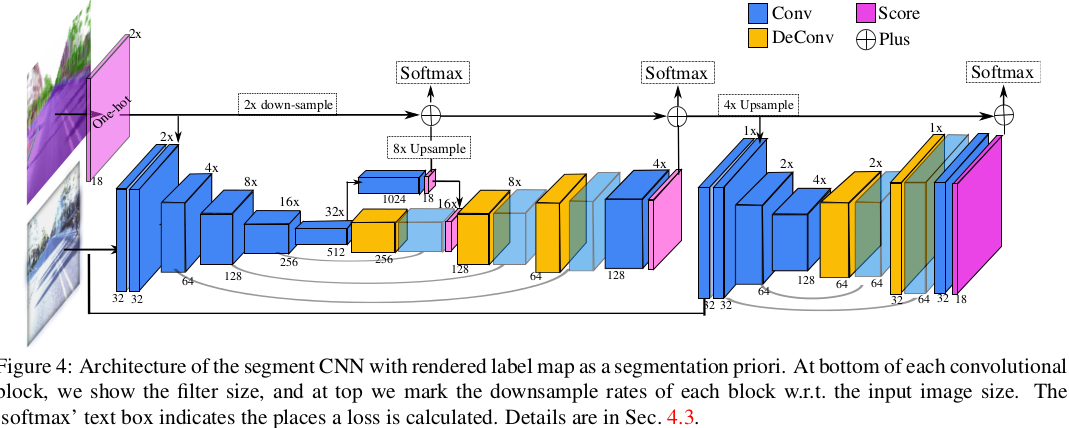
\includegraphics[width=0.95\textwidth]{SemanticSLAM/DeLS2.png}
\caption{Segment Network in DeLS}
\label{SegmentDeLS}
\end{figure}

需要注意的是,当标签地图加入框架时,需要经过编码,即每一个像素经One-hot操作得到一个32维的Feature Representation。然后得到的32维特征加入到RGB图像的第一层卷积输出中,且该层的Kernel数也是32个,从而平衡了两种数据的通道数(Channel Number)。

\subsection{Experiment}

\begin{itemize}
\item Adopt OpenGL to efficiently render a label map with the z-buffer handling. 

\item Implement all the networks by adopting the MXNet platform.

\item 使用RNN可以提高Pose的精度,也可以提高Segment的精度,尤其对于纤细的物体。

\end{itemize}

\subsection{Conclusion}

基于已有的3D语义地图以及视频数据,实现相机的姿态、场景语义任务的实现。算法融合了多种传感器信息。实验表明,相机位姿估计与场景语义两类任务可以相互促进、提高。

\section{PAD-Net: Multi-Task Guided Prediction-and-Distillation Network for Simultaneous Depth and Scene Parsing \cite{Xu2018PADNet}}

\subsection{Abstract}

利用同一个网络,完成深度估计与场景解析两个任务。具体来说,通过神经网络学习一系列的中间辅助任务(Intermediate Auxiliary Tasks),然后基于中间任务的输出,作为多模式数据(Multi-modal  input)输入到下一层网络中,完成最终的深度估计以及场景解析两个任务。

其中,一系列的中间任务包括低层任务和高层任务。低层任务包括:Surface Normal, Contour;高层任务包括:Depth Estimation, Scene Parsing.

\subsection{Analysis}

\subsubsection{Effect of Direct Multi-task Learning}
It can be observed that on NYUD-v2, the Front-end + DE + SP slightly outperforms the Front-end
+ DE, while on Cityscapes, the performance of Front-end + DE + SP is even decreased, which means that using a direct multi-task learning as traditional is probably not an effective means to facilitate each other the performance of different tasks. (DE: Depth Estimation, SP: Scene Parsing)

\subsubsection{Effect of Multi-modal Distillation}
这种Multi-Modal Distillation对结果十分有效。且:
\begin{quote}
By using the attention PAD-Net (Distillation C + SP) guided scheme, the performance of the module C is further improved over the module B.
\end{quote}

\subsubsection{Importance of Intermediate Supervision and Tasks}

测试了选择不同的中间任务类型,如:(Multi-Task Deep Network)MTDN + inp2(depth + semantic map), MTDN+3inp3(depth + semantic + surface normal), MTDN + all(depth + semantic + surface + contour).

其中MTDN + all比MTDN + 0-3都好。

\section{RNN for Learning Dense Depth and Ego-Motion from Video}

参考文献:\cite{Wang2018DenseSLAMNet}

{\color{red}时间:2018年05月19日}

\subsection{Abstract}

现在基于学习的单目深度估计,在Unseen Dataset上泛化较差,可以利用连续两帧之间的特征匹配来解决。本文提出了基于RNN的多目视觉深度估计以及运动估计。结果表明,在远距离上的深度估计,表现很好。本文方法可使用both static and deformable scenes with either constant or inconsistent light conditions.

\subsection{Introduction \& Related Works}

由于CNN只能捕获单帧内部的空间特征,所以即使输入两帧图像,实际效果也比较差。相关的SLAM框架有:

\begin{itemize}
\item ORB-SLAM, DSO: 稀疏SLAM
\item LSD-SLAM: semi-dense SLAM,利用光强来实现跟踪以及构建地图
\item DTAM: dense SLAM
\end{itemize}

上述框架仅适用于静态、光照恒定、足够的camera motion baseline的情景。

进来,CNN可被用于SLAM中的以下部分:
\begin{itemize}
\item Correspondence matching
\item Camera Pose estimation
\item Stereo
\end{itemize}
输出包括:
\begin{itemize}
\item Depth maps
\item point clouds and voxels
\end{itemize}
CNN的优势在于可以适用于纹理较少、表面覆盖、很细等场景下,这些场景对纯使用几何技术来说很难实现。

Newcombe研究表明,多目视觉有助于提高深度估计的精度,而本文作者认为采用相邻几帧可以实现类似的效果。

有作者利用一个非监督生成模型来学习复杂的3D到2D的投影。但这些手段不太适用于Deformable Objects.

\subsection{Network Architecture}

\begin{figure}[!htbp]
\centering
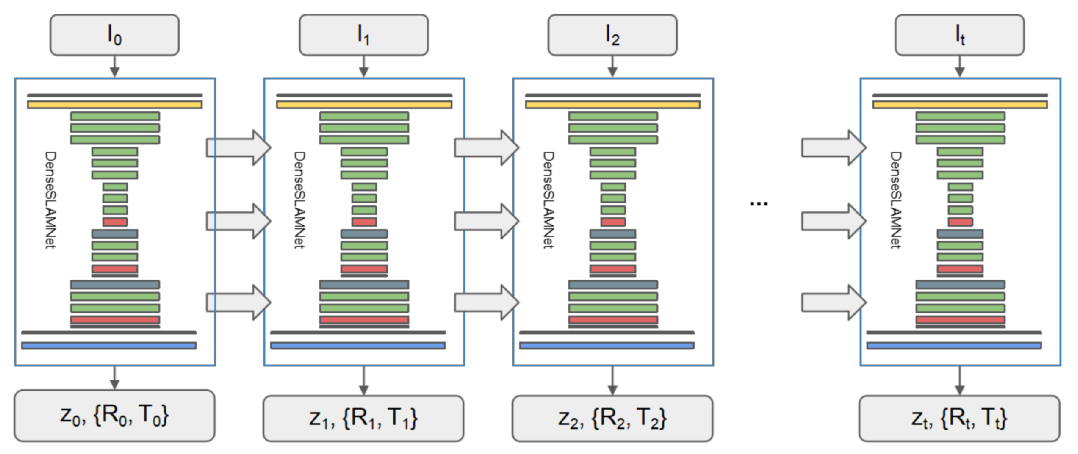
\includegraphics[width=0.95\textwidth]{SemanticSLAM/DenseSLAMNet1.png}
\caption{Dense SLAM框架}
\label{DenseSLAMNet1}
\end{figure}

从图\ref{DenseSLAMNet1}可以看出,它接受当前RGB图像$I_t$以及来自迁移级的隐藏状态$h_{t-1}$。$h_{t-1}$通过LSTM单元进行内部转移。网络的输出是稠密地图$z_t$以及相机的姿态$R_t, T_t$等。有没在每一时刻,只输入一帧图像,且输出该帧对应的深度以及姿态,所以相比于CNN具有更高的灵活性。

具体的每一块的细节结构如下:

\begin{figure}[!htbp]
\centering
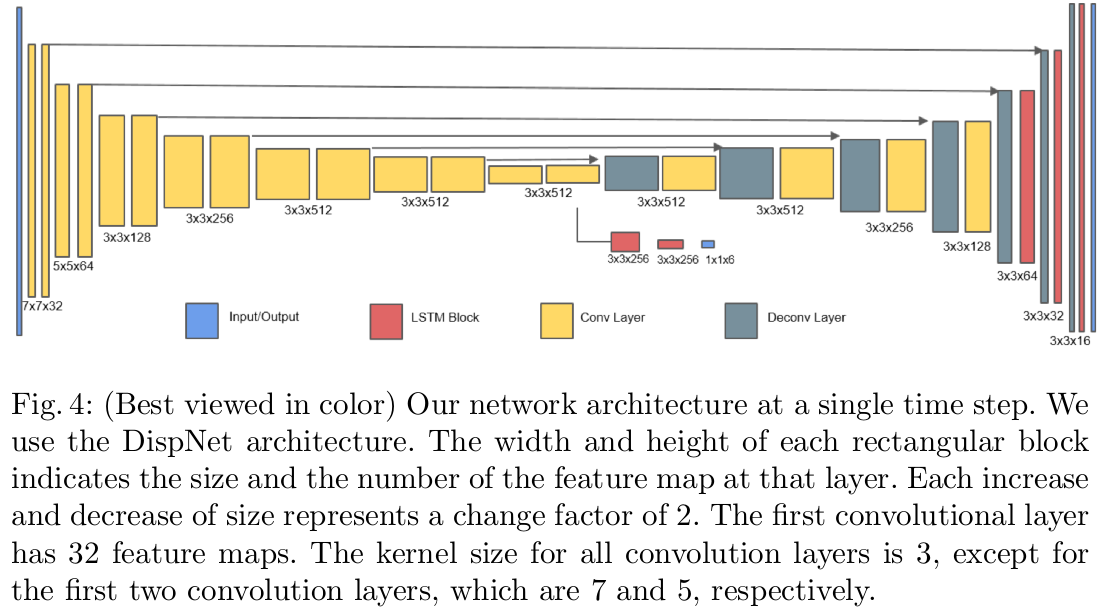
\includegraphics[width=0.95\textwidth]{SemanticSLAM/DenseSLAMNet2.png}
\caption{Dense SLAM中每一级的细节框架}
\label{DenseSLAMNet2}
\end{figure}

网络结构的另一个参数是时间窗口的大小$N$。本文中$N=10$,也就是说,图\ref{DenseSLAMNet2}中的结构被重复十次。

\subsection{Training}

During training, we feed
frames to the network and compute losses from all frames in a temporal window. However, there is no input length constraint at test time.

\subsubsection{Loss Function}

由三部分组成:
\begin{itemize}
\item A Point-wise depth loss

\begin{displaymath}
L_{depth} = \sum_{t}^{N}\sum_{i, j}\left\| \xi_t(i, j) - \hat{\xi}_t(i, j) \right\|_{L1}
\end{displaymath}
其中,$i, j$为索引,$t$为time step.使用$L1-Norm$的原因是,它对噪声更鲁棒。

\item a camera pose loss

Use the Euler angle $R$ 和平移向量$T$。

\begin{displaymath}
\begin{gathered}
L_{rot} = \sum_{t}\left\| r_t - \hat{r}_t \right\|_2 \\
L_{trans} = \sum_{t}\left\| t_t - \hat{t}_t \right\|_2
\end{gathered}
\end{displaymath}

\item a scale-invariant gradient loss

为了保证深度图的Smoothness和Sharpness,所以增加了这个loss。具体如下:
\begin{displaymath}
L_{grad} = \sum_{t}\sum_{h\in\{ 1, 2, 4, 8, 16 \}}\sum_{i, j}\left\| g_{h, t}(i, j) - \hat{g}_{i, j}(i, j)\right\|_2
\end{displaymath}
其中,$h$代表不同的尺度。$g_{h, t}$is a scale-normalized, discretized measurement of the local changes of $\xi_t$。定义如下:
\begin{displaymath}
g_{h, t} = \left( \frac{\xi_t(i+h, j) - \xi_t(i, j)}{|\xi_t(i + h, j) + \xi_t(i, j)|}, \frac{\xi_t(i, j+h) - \xi_t(i, j)}{|\xi_t(i, j+h) + \xi_t(i, j)|}    \right)
\end{displaymath}

$L_{grad}$emphasizes the depth discontinuities, such as occlusion
boundaries and sharp edges, as well as the smoothness in homogeneous regions.
This property encourages the estimated depth map to preserve more details and
reduce noise. Therefore, we put highly weight on this component of the loss. 这一项在所有的Loss中比重较大。

\end{itemize}

最终的Loss由上面几项的和构成:
\begin{displaymath}
L = \alpha * L_{depth} + \beta * L_{pose} + \gamma * L{grad}
\end{displaymath}
其中,$\alpha, \beta, \gamma$是系数,由经验决定。


注意,下面解释的是为什么使用Disparity而不是直接使用深度。
\begin{quote}
{\color{red} \textbf{Caution!} Disparity, the reciprocal of depth (深度的倒数), $\xi = \frac{1}{z}$  as our direct estimation because it can represent points at infinity and account for the localization uncertainty of points at increasing
distance.}
\end{quote}

Different datasets have different camera intrinsic parameters, so we
explicitly crop and resize images to ensure uniform intrinsic parameters. This
step assures that the non-linear mapping between color and depth is consistent
across all training datasets.

\subsection{Experiments}

We evaluate DenseSLAMNet using five error metrics。具体可以参考文章。
\begin{itemize}
\item Sc-inv
\item Abs-rel, Abs-inv
\item RMSE, RMSE-log
\end{itemize}

\subsection{Ablation Studies}

比较了三种不同的网络结构。
\begin{enumerate}
\item CNN-SINGLE, 去掉图\ref{DenseSLAMNet2}中LSTM单元
\item CNN-STACK, 使用与CNN-SINGLE相同的网络,但是输入stack of ten images as input.
\end{enumerate}

实验结果表明,LSTM可有效保留时间域的信息,从而深度预测的更好。

\subsubsection{Conclusions}

引入了LSTM单元。
Our method effectively utilizes the temporal relationships between neighboring
frames through LSTM units, which we show is more effective than simply stack-
ing multiple frames together as input.

比几乎所有的单帧CNN-based 都好。
Our DenseSLAMNet outperformed nearly
all of the state-of-the-art CNN-based, single-frame depth estimation methods on
both indoor and outdoor scenes and showed better generalization ability.


\section[DA-RNN]{DA-RNN: Semantic Mapping with Data Associated Recurrent Neural Networks}

参考文献:\cite{Xiang2017DARNN}

{\color{red} \textbf{评语} 看得出来,RNN在帮助建立相邻帧之间的一致性方面具有很大的优势。}

本文利用可以实现Data Associate的RNN产生Semantic Label。然后作用于KinectFusion,来插入语义信息。

所以本文利用了RNN与KinectFusion来实现语义地图的构建!

\subsection{Related Works}

{\bfseries 本文提出的 DA-RU (Data Associated Recurrent Unit) 可以作为一个单独的模块加入到已有的CNN结构中!}

\subsection{Methods}

需要注意到是,本文采用了DA-RNN与KinectFusion合作的方式来产生最终的Semantic Mapping,而文章采用的则是ORB-SLAM与CNN结合,他们有一些共同的结构,如Data Associate,虽然我现在还不明白这个DA具体得怎么实现!?

\subsection{Experiments}

实验表明,针对不同的实验输入场景,RGB图像和Depth图像可能发挥不同的作用,有一些时候甚至让结果更差,而本文采用Contatenated把来自于RGB和Depth的Feature进行组合起来,在这里,是否可以采取Attention或者\cite{Xu2018PADNet}中采用的Knowledge Distillation的方式进行多模态数据融合呢!?

此外,实验中也发现,有时候RGB图像的Color会影响实验结果,所以,是否可以利用一些其它的不那么Confusing的数据呢,比如Shape等,这也类似于\cite{Xu2018PADNet}中多任务中的Contour类似吧!


\subsection{Conclusion}

\begin{itemize}
\item $\star$将来的可以借助Optical Flow来生成图像帧之间的Data Associate,来代替KinectFusion的作用!
\end{itemize}

\section{SemanticFusion: Dense 3D Semantic Mapping with CNNs}
参考文献:\cite{SemanticFusion2016}

主要框架,用到了ElasticFusion和CNN来产生稠密的Semantic Mapping.

\subsection{Introduction \& Related Works}

本文的算法,利用SLAM来实现2D Frame与3D Map之间的匹配(Corresponding)。通过这种方式,可以实现把CNN的语义预测以概率的方式融合到Dense semantically annotated map.

为什么选择ElasticFusion呢,是因为这种算法是surfel-based surface representation,可以支持每一帧的语义融合。

比较重要的一点是,通过实验说明,引入SLAM甚至可以提高单帧图像的语义分割效果。尤其在存在wide viewpoint variation,可以帮助解决单目2D Semantic中的一些Ambiguations.

之前存在方法使用Dense CRF来获得语义地图。

本文的主要不同是:利用CNN来产生语义分割,然后是在线以 Incremental 的方式生成Semantic Map。即新来一帧就生成一帧的语义地图。

\subsection{Method}

系统由三部分组成:
\begin{itemize}
\item A real-tiem SLAM system ElasticFusion

用于提供帧间的关联、全局一致的地图

\item CNN

产生语义分割

\item Bayesian update scheme

基于SLAM提供的Pose关系、CNN提供的每个像素的Class Probability对Map中的每一个surfel的Class Probability进行更新!

\end{itemize}

此外,作者还尝试了用CRF来利用SLAM提供的Geometry帮助语义分割。

非常粗糙的流程图如下图所示:
\begin{figure}[!hbtp]
\centering
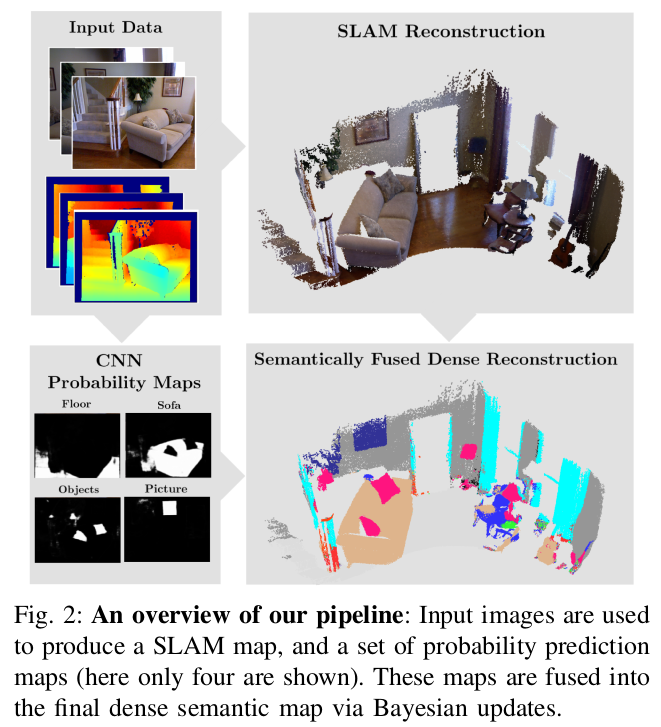
\includegraphics[width=0.75\textwidth]{SemanticSLAM/SemanticFusion0.png}
\caption{粗糙的数据流图}
\label{SemanticFusion0}
\end{figure}

\subsubsection{SLAM Mapping}
就是使用ElasticFusion.

\subsubsection{CNN Architecture}

使用Deconvolutional Semantic Segmentation network,与FCN同年提出的另一个分割网络。

在本实验中,输入由RGB变为RGBD,多了一个Channel.然而,深度相关的训练数据比较少,为了提高利用率,作者利用其它三个输入的光强的平均值对Depth Filter进行初始化。

对输入数据,作者还进行了Scaling, RGB是用Bilinear Interpolation, Depth数据是Nearest enighbour。

\subsubsection{Incremental Semantic Label Fusion}

在生成的地图$\mathcal{M}$中,每一个Surfel(ElasticFusion的结果)不仅代表了Location、Normal等信息,还包含一个类别($\mathcal{L}$)的分布。

输入数据为$\mathbf{I}_k$表示RGB图像与Depth等。

在对每一个Surfel进行类别分布概率更新时,采用的Recursive Bayesian update,这个算法就是Probability Robotics里面最基础的算法,也就是分为Prediction和Correlation两个步骤。

\begin{displaymath}
P(l_i | I_{1, \ldots, k}) = \frac{1}{Z}P(l_i | I_{1, \ldots, k- 1})P(O_{u(s, k)=l_i | I_k})
\end{displaymath}

其中,第一个$P$表示根据过去的信息的预测,在这里也就是已有的$\mathcal{M}$里面的一个surfel的class probability,如果,是一个全新的Surfel,则初始化它为均匀分布,因此这样熵最大;而第二个$P$表示来自CNN输入是$I_k$时输出的class probability,然后对已有地图中的surfel的class probability进行Correlation!

\subsubsection{Map Regularisation}

作者尝试了利用CRF来借助map geometry对预测的Semantic surfel进行Regularise。

在这里,把每一个Surfel当做CRF的一个Node。

这一部分,参考论文吧。

\subsection{Experiments}

本文用到的Semantic分割的方法(CNN + SLAM)与普通的单CNN相比,具有很大的优势。本文的方法是,得到3D的Semantic Map后,重投影到2D图像中。

时间方面,SLAM需要29.3ms,CNN的前向传播用了51.2ms,Bayesian更新用了41.1ms。

\subsection{总结}

未来也还是SLAM与语义分割相互促进吧,达到Semantic SLAM。


\section{Meaningful Maps with Object-Oriented Semantic Mapping}
参考文献:\cite{Meaningful2016}

主要的框架是,利用CNN与ORB-SLAM2来实现Semantic Mapping。{\bfseries 但是都用到了Data Association的操作}!而且本文还是Object-oriented (Instance level) !

\subsection{Introduction \& Related Works}

{\bfseries 重要:}

与已有的方式不同的是,本文的算法不仅分割独立的3D Point,也就是把语义信息投影到3D Point中,而是投影到3D Structure。这样会更有利于场景理解。

已有的SLAM算法得到的结果都是一些几何上的概念,比如:点、面、表面等。另一方面,为了实现与环境交互,必须基于语义地图才行。

\subsubsection{Semantic Mapping}

语义信息与地图构建可能属于两个不同的过程得到。

有一些算法用到了HMM或Dense CRF等。

\subsubsection{Object Detection and Semantic Segmentation}

FCN的缺点是,形成的语义地图一般缺少Notion of independent object instances. 如果只是Pixel-level的labels不能辨别有重叠时物体的身份。

也有一些Instance-level的分割算法,但精度、速度都有待提高。

\subsection{Object Oriented Semantic Mapping}

算法的主要步骤:
\begin{figure}[!hbtp]
\centering
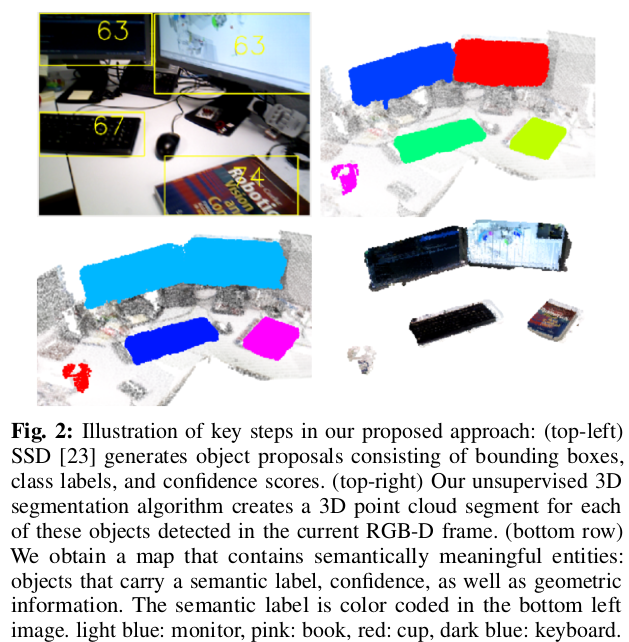
\includegraphics[width=0.75\textwidth]{SemanticSLAM/OrientedMap0.png}
\caption{算法的几个主要步骤}
\label{OrientedMap0}
\end{figure}

算法使用RGB-D作为输入,算法是用ORB-SLAM2提供相机的姿态、地图等。

\subsubsection{Object Detection for Semantic Mapping}

本文使用SSD来完成Object的Location和 Recognition。

\subsubsection{3D Segmentation}

由于需要非常精确的图像分割,所以本文利用Depth图来帮助分割。所以需要对Depth进行分割的算法,本文采用了文章\cite{Felzenszwalb2004}\cite{Pham2016Geometrically}等人的算法。也是涉及到基于图的分割的过程。

\subsubsection{Data Association}

重点。

当完成了把3D Point投影到识别的物体后,数据关联要做的事:判断检测到的物体是否已经在已经构建的地图中存在了呢,如果不存在的话,就需要新增这个物体。

通过一个二阶的流程来实现:

\begin{itemize}
\item 对于每一个检测到的Object,根据点云的欧式距离,来选择一系列的Landmarks(已经检测到并在地图里面已经有的Object)
\item 对Object和Point Cloud of landmark进行最近邻搜索,使用了k-d tree来提高效率,其实这一步也就是判断当前图像检测到的Object与已有的地图中的Landmark(Object)是否相匹配。
\end{itemize}

在第二步中,如果多余50 \% 的Points的都距离小于2cm的话,就说明这个检测到的Object已经存在了。

这个也就是把CNN的分割结果与地图中的Object进行关联起来,并用颜色表示Map中Object的类别。

\subsubsection{Object Model Update}

地图中的目标保存:
\begin{itemize}
\item 与目标相关联的分割的3D点云
\item ORB-SLAM中因子图的各个位姿的索引
\item 有SSD提供的各个目标的置信度
\end{itemize}

\begin{figure}[!hbtp]
\centering
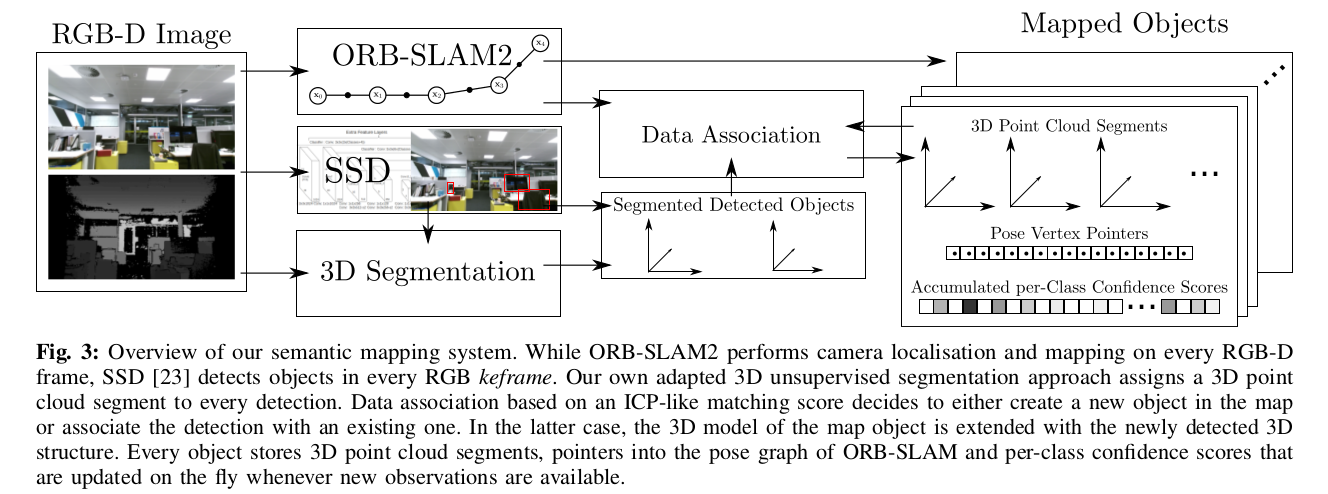
\includegraphics[width=0.95\textwidth]{SemanticSLAM/OrientedMap1.png}
\caption{Semantic Mapping 系统概览}
\label{OrientedMap1}
\end{figure}

上图中可以看出,


{\color{red} \textbf{评语}:在上一篇SematicFusion中,采用的Recursive Bayesian 的更新规则来完成地图更新的!看来,这个是CNN与传统的SLAM框架结合的时候的一个需要解决的问题,那就是如何把新来的物体与已有的地图中的物体相互关联起来,并更新!}

\subsubsection{Map Generation}

通过保存Keyframe中物体的3D poin clouds、每一个物体的3D分割以及执行位姿图中的一个指针。

\subsection{总结}

未来可以的发展方向:
\begin{itemize}
\item 语义Landmark如何提高SLAM的精度,从而实现Semantic SLAM
\item 把稀疏的语义地图改进为稠密地图
\end{itemize}

\section[LiteFlowNet]{LiteFlowNet: A Lightweight Convolutional Neural Nework for Optical Flow Estimation}

参考文献:\cite{Hui2018LiteFlowNet}, CVPR 2018

\subsection{背景知识}

FlowNet2是基于CNN进行光流估计的SOTA算法(?), 需要160M的参数量。LiteFlowNet实现了30倍的轻量化,并且比FlowNet2块1.36倍。

主要的贡献:
\begin{itemize}
\item 在每一层金字塔(Pyramid Level)预测光溜更高效的轻量级联网络。通过早前矫正(Early Correction)提高了精度,同时无缝支持网络中的描述子匹配。
\item 提出了一个新型的光流正则化层,可以改善野值点、光流边界模糊等问题,是基于特征驱动的区域卷积实现
\item 网络结构可以高效提取Pyramidal Feature以及Feature Warping,而不是像FlowNet2中的Image Warping。
\end{itemize}

FlowNet2通过级联FlowNet,来不断调优光流场, by contributing on the flow increment between the first image and the warped second imaeg?

后来,SPyNet通过在每一Pyramid level采用Imae Warping实现了只有1.2M大小的网络,但精度只有FlowNet大小,而达不到FlowNet2的水平。

{\bfseries Image Warping: 图像扭转,是一种数字图像处理过程,在任何图像中所描述的任何形状都会产生显著有损。扭曲可用于矫正图像有损,同时可用于某种创意目的。纯粹的图像扭曲意味着点到点的映射,而不改变其颜色。}

提高FlowNet2以及SPyNet的两种准则(Principles):

\begin{itemize}
\item Pyramid feature extraction

Consists of an encoder and a decoder. Encoder把输入的图像对分别映射到多尺度高维特征空间中;Decoder以Coarse-to-fine的框架估计光流场。这比FlowNet2采用U-Net更轻量化。相比于SPyNet,我们的模型把特征提取与光流估计两个过程分离,可以更好的处理精度与复杂度之间的矛盾。

\item Feature Warping

FlowNet2与SPyNet将输入图像对中的第二幅图像基于先前估计的光流进行Warp,然后使用Warped的第二幅图像与第一幅图像的特征图谱Refine估计的光流。

所以这个过程中,首先把第二幅图像进行Warp,然后提取Warp图像的特征,这个过程十分繁琐。所以,本文提出直接对Feature Map进行warp。保证模型更精确以及高效。

\end{itemize}

更详细的细节一定要看原文\cite{Hui2018LiteFlowNet}。

此外,除了上面两个主要改进的 Principle, 作者还提出第三个比较重要的改进措施,那就是 Flow Regularization.

\begin{itemize}
\item Flow Regularization

级联的光流估计类似于能量最小化方法中的保真度(Data Fidelity)的作用。 为了消除边界的模糊以及野值点,Regularize flow Field的常用Cues:
\begin{itemize}
\item Local flow consistency
\item Co-occurrence between flow boundaries
\item Co-occurrence between intensity edges
\end{itemize}

对应的代表方法包括:
\begin{itemize}
\item Anisotropic image-driven
\item image- and flow-driven
\item Complementary regularizations
\end{itemize}

在本文中,提出的是Feature-driven local convolution layer at each pyramid level. 该方法对Flow-以及Image-敏感。

{\color{red} \textbf{评语}:看起来,一个是提高精度,一个是提高效率,这是两个最终的目的。提高精度可以通过设计网络结构以及增加其它考虑来实现;提高效率的一个重要表现是降低模型的参数数量,提高运算速度。不过,本文虽然参数数量减少了30倍,但速度却只提高了1.36倍,这里面的原因是什么?}

\end{itemize}

\subsection{Related Works}

\subsubsection{Variational Methods}

Address illumination changes by combining the brightness and gradient constancy assumptions.

DeepFlow, propose to correlate multi-scale patches and incorporate this as the matching term in functional.

PatchMatch Filter, EpicFlow.

本文提出的网络结构,是受Variational methods中的Data Fidelity以及正则化启发。

\subsubsection{Machine Learning Methods}

PCA-Flow. 这些参数化模型可以通过CNN高效的实现。

\subsubsection{CNN-based Methods}

FlowNet, 使用能量最小化作为后处理步骤,来降低在光流边界的平滑效应。不能端到端训练?

FlowNet2, 通过FlowNet的级联实现。虽然提高了精度,但模型更大,计算更复杂。

SPyNet,受Spatial Pyramid启发,模型更紧凑,但效果远不如FlowNet2。

InterpoNet, 借助第三方系数光流但需要off-the-shelf的边缘检测。

DeepFlow, 使用Correlation而不是真正意义的CNN,参数不能训练。

\subsubsection{Establish Point Correspondence}

Establishing point correspondence, 一种方式是Match Image Patches

CNN-Feature Matching, 首先被Zagoruyko等人提出(Learning to compare image patches via CNN, 2015 CVPR)。

MRF-based, G$\ddot{u}$ney等人提出利用Feature Representation以及利用MRF来估计光流。

Bailer使用多尺度Feature,然后以类似于Flow Fields的方式进行特征匹配。

Fischer和Ilg等人为了提高计算效率,仅在稀疏空间维度进行特征匹配。

本文中,We reduce the computational burden of feature matching by using a short-ranged matching of warped CNN features at sampled positions and a sub-pixel refinement at every pyramid level.

类似于Spatial Transformer, 本文利用 f-warp layer来区分不同个Channel.本文的决策网络是一个更普用的Warping Network,可以用来Warp高层次的CNN Features,而不仅仅是对Image进行Warpping.


\subsection{LiteFlowNet}

整体结构如下:
\begin{figure}[!hbtp]
\centering
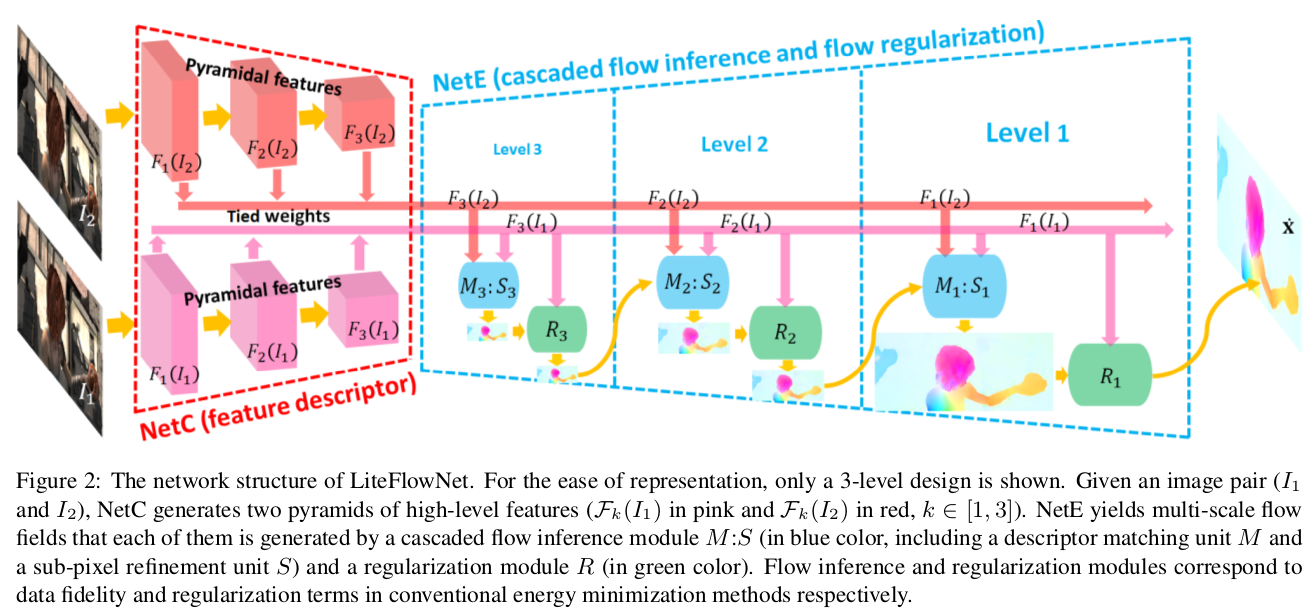
\includegraphics[width=0.95\textwidth]{SemanticSLAM/LiteFlowNet0.png}
\caption{LiteFlowNet结构框图}
\label{LiteFlowNet0}
\end{figure}

\subsubsection{Pyramid Feature Extraction}

进行stride-$s$的卷积操作,得到的Feature Map表示为:$\mathcal{F}_k(I_i)$,即第$i$个图像的第$k$层Feature Map。简化写成 $\mathcal{F}_i$。

\subsubsection{Feature Warping (f-warp)}

假设\.x为预测的光流,则Feature Warping是指:
\begin{displaymath}
\tilde{\mathcal{F}}_2(x) \triangleq \mathcal{F}_2(x + \dot{x}) \sim \mathcal{F}_1(x) 
\end{displaymath}

注意,Warping是作用于$\mathcal{F}$上的,而不是输入图像上的。

为了使上述过程可以支持end-to-end训练,这里采用Bilinear Interpolation进行插值的技术实现Warping。Bilinear Interpolation是支持后向传播训练的!修改后Warping实现公式如下:
\begin{displaymath}
\tilde{\mathcal{F}} = \sum_{x_s^i \in N(x_s)} \mathcal{F}(x_s^i)(1-|x_s - x_s^i|)(1 - |y_s - y_s^i|)
\end{displaymath}

其中,$x_s = x + \dot{x} = (x_s, y_s)^T$是输入的源Feature Map中的坐标。$x$denotes the target coordinates of the regular grid in the interpolated feature map $\mathcal{F}$,$N(x)$代表the four pixel neighbors of $x_s$.

自己的理解:首先$x$是插值后 的图像索引,而$x_s = x + \dot{x}$是插值前Feature Map中对应Object Feature的$x$索引处的索引。$x_s^i$是在$x_s$周围的四个紧邻像素。也就是个Bilinear Interpolated.

\subsubsection{Cascaded Flow Interface}

{\color{red} \textbf{评语}:这一块看的比较吃力。为什么会吃力?因为新的概念么?那么作者为什么提出这么麻烦的概念呢?实际效果又怎么样呢?}

通过计算高层特征向量的Correlation来实现输入图像的点对应。

\begin{displaymath}
c(x, d) = \mathcal{F}_1(x) \cdot \mathcal{F}_2(x + d) / N
\end{displaymath}
这个公式跟FlowNet中的计算方式区别不大。只不过这里的$N$是指Feature的长度。

\begin{figure}[!hbtp]
\centering
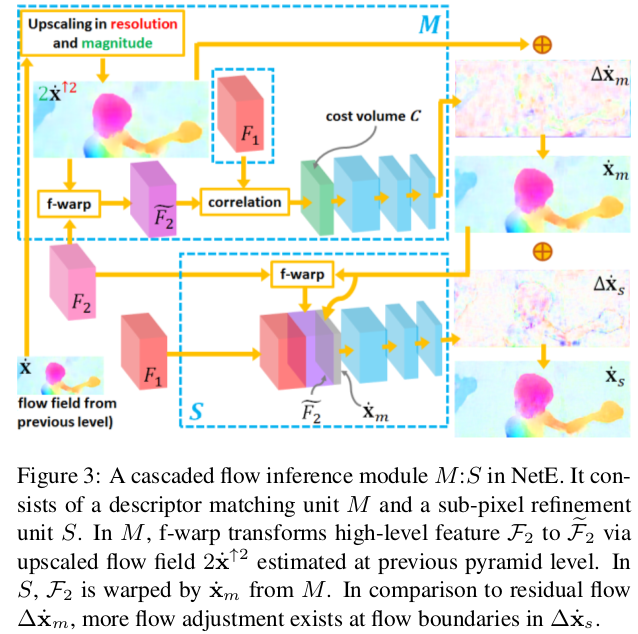
\includegraphics[width=0.75\textwidth]{SemanticSLAM/LiteFlowNet1.png}
\caption{在NetE中的级联光流推理模块,M:S}
\label{LiteFlowNet1}
\end{figure}

\textbf{M Module}$\;$  在Descirptor Matching unit M, Residual flow $\varDelta \dot{x}_m$. A complete flow field $\dot{x}_m$ is computed as follows, 这句话没懂

\begin{displaymath}
\dot{x}_m = \underbrace{M(C(\mathcal{F}_1, \tilde{\mathcal{F}}_2; d))}_{\varDelta \dot{x}_m} + s\dot{x}^{\uparrow s}
\end{displaymath}

其中,$\dot{x}$是上一层的最开始的光流估计!

\textbf{S Module}$\;$ 
为了进一步提高flow estimate  $\dot{x}_m$ 的精度,即达到亚像素级别。作者引入了Second flow inference。 这可以防止错误光流的放大并传到下一级。Sub-pixel refinement unit $S$,会产生一个更准确的光流场,这通过最小化$\mathcal{F}_1$和 $\tilde{\mathcal{F}}_2$之间的距离来实现。

\begin{displaymath}
\dot{x}_s = \underbrace{S(C(\mathcal{F}_1, \tilde{\mathcal{F}}_2, \dot{x}_m))}_{\varDelta \dot{x}_s} + \dot{x}_m
\end{displaymath}

{\bfseries 所以总的来说} M模块是为了计算$\varDelta \dot{x}_m$, 而$S$模块是为了计算$\varDelta \dot{x}_s$。对最开始$\dot{x}$估计的光流进行两次的Refinement.

\subsubsection{Flow Regularization}

这一部分主要消除光流边界的模糊、存在的artifacts等。提出用 feature-driven local convolution (f-lcon)

假设Feature Map (F)的尺寸为:$M * N * c$,定义f-lcon的滤波器为$\textbf{G}={g}$

对于输入为$\dot{x}_s$, Flow Regularization值的是:
\begin{displaymath}
\dot{x}_r = R(\dot{x}_s; G)
\end{displaymath}
输出的是正则化后的光流估计$\dot{x}_r$

下面的关键是如何生成这个用于正则化的卷积核。为此,作者定义了一个feature-driven的距离度量$\mathcal{D}$,总的来说,该度量由一个CNN unit $R_D$来计算:
\begin{displaymath}
\mathcal{D} = R_D(\mathcal{F}_1, \dot{x}_s, O)
\end{displaymath}

基于这个度量,可以计算得到卷积核:
\begin{displaymath}
g(x, y, c) = \frac{\exp(-\mathcal{D}(x, y, c)^2)}{\sum_{(x_i, y_i)\in N(x, y)}\exp(-\mathcal{D}(x_i, y_i, c)^2)}
\end{displaymath}

其中$N(x)$表示一个$\omega * \omega$的近邻。

\subsection{Ablation Study}

算法的结果是优于 FlowNet2, SPyNet等。

\subsubsection{Feature Warping}

没有Warping, 光流更Vague.通过计算residual flow (M:S两个模块的功能)可以提高估计效果。

M: Matching

S: Sub-pixel refinement

R: Regularization units in NetE

\subsubsection{Descriptor Matching}

\subsubsection{Sub-Pixel Refinement}

The flow field generated from
WMS is more crisp and contains more fine details than
that generated from WM with sub-pixel refinement dis-
abled.

更小的flow artifacts.

\subsection{Regularization}

In comparison WMS with regularization
disabled to ALL, undesired artifacts exist in homogeneous
regions

Flow bleeding and
vague flow boundaries are observed.

表明, Feature-driven local convolution对于光滑光流场、保持crisp flow boundaries非常重要!

\subsection{Conclusion}

Pyramidal feature extrac-
tion and feature warping (f-warp) help us to break the de
facto rule of accurate flow network requiring large model
size. To address large-displacement and detail-preserving
flows, LiteFlowNet exploits short-range matching to gener-
ate pixel-level flow field and further improves the estimate
to sub-pixel accuracy in the cascaded flow inference. To
result crisp flow boundaries, LiteFlowNet regularizes flow
field through feature-driven local convolution (f-lcon). With
its lightweight, accurate, and fast flow computation, we ex-
pect that LiteFlowNet can be deployed to many applications
such as motion segmentation, action recognition, SLAM,
3D reconstruction and more.


\section{小结}

2018.05.23小结

在生成Semantic Map的时候,看样子现在的趋势,是利用RNN保证时间一致性;利用多模态数据提高精度,但如何融合多模态数据的Feature有待研究,现有的有一些是直接Concatenate、Knowledge Distillation、Attnetion(?)等机制。


\section{ExFuse: Enhancing Feature Fusion for Semantic Segmentation}

参考文献:\href{https://zhuanlan.zhihu.com/p/37177073}{ExFuse简介-知乎}

\subsection{要解决的问题}

在语义分割领域中,经常需要融合多层的Feature。然而,底层的Feature含有的语义信息较少,但分辨率较高,噪声也比较少,这是由于卷积层比较浅;而高层的Feature语义信息多,但空间分辨率很小。

所以本文就提出了:1)增加底层特征的语义;2) 在高层中增加空间信息

\subsection{Method}

使用了ResNet、GCN(Global Convolution Net)的思想。

\begin{figure}[!hbtp]
\centering
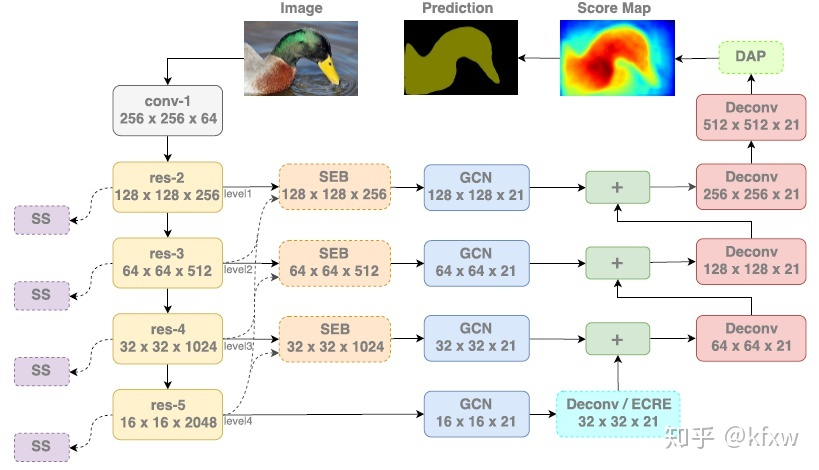
\includegraphics[width=0.95\textwidth]{SemanticSLAM/ExFusion0.jpg}
\caption{ExFusion的实现框图}
\label{ExFusion0}
\end{figure}

其中,SS, SEB, ECRE, DAP是文章作者提出的算法。

\subsubsection{在底层中加入更多的语义信息}
具体是三个方面的改进:
\begin{itemize}
\item Layer Rearrengement

 ResNeXt网络结构中,各级的网络包含的残差单元个数为{3,4,23,3}。为了提高底层特征的语义性,一个想法便是让低层的两级网络拥有的层数更多。因此作者将残差单元个数重排为{8,8,9,8},并重新在ImageNet上预训练模型。重排后网络的分类性能没有明显变化,但是分割模型可以提高约0.8个点(mean intersection over union)的性能。

\item Semantic Supervision(SS)

深度语义监督其实在其他的一些工作里(如GoogLeNet,边缘检测的HED等等)已经使用到了。这里的使用方法基本上没有太大变化,能够带来大约1个点的提升。

\item Semantic Embedding branch(SEB)

\begin{figure}[!hbtp]
\centering
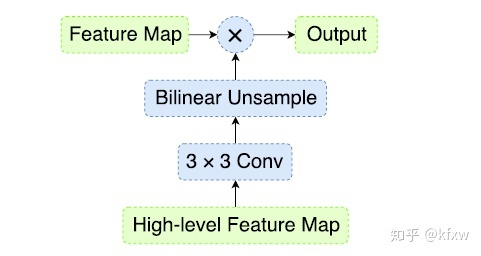
\includegraphics[width=0.65\textwidth]{SemanticSLAM/ExFusion1.jpg}
\caption{语义嵌入分支的结构图}
\label{ExFusion1}
\end{figure}

 其做法是将高层特征上采样后,与低层特征逐像素相乘,用在GCN之前。该部分能带来大约0.7个点的提升。

\end{itemize}

\subsubsection{在高层中加入更多的空间信息}

用两种方法来把更多的空间信息融入到高层特征中:
\begin{itemize}
\item 通道分辨率嵌入(Explicit Channel resolution embedding, ECRE)

其思路是在上采样支路中使用[2,3,4]工作中都使用到的子像素上采样模块(sub-pixel upsample)。作者的出发点并不是前人工作中强调的如速度快、消除反卷积的棋盘效应等等,而是通过这个结构能够让和空间信息相关的监督信息回传到各个通道中,从而让不同通道包含不同空间信息。该模块和原有的反卷积一起使用才能显示出更好的性能。同单独使用反卷积相比,性能可以提高约0.6个点。

\item 稠密邻域预测(Densely adjacent prediction, DAP)

DAP模块只使用在输出预测结果的时候。其想法也是通过扩展通道数来增加空间信息。举一个例子来描述其功能,假设DAP的作用区域为3x3,输出结果的通道数为21,则扩展后的输出通道数为21x3x3。每3x3个通道融合成一个通道。如在最终结果中,第5通道(共21通道)的(12,13)坐标上的像素,是通过DAP之前的第5+0通道(11,12)、5+1通道的(11,13)、5+2通道的(11,14)、5+3通道的(12,12)、5+4通道的(12,13)、5+5通道的(12,14)…平均得到的。DAP能带来约0.6个点的提升。

\end{itemize}

\section{Multi-View Deep Learning for Consistent Semantic Mapping with RGB-D Cameras}

{\color{red} 时间:2018.05.24}

主要的贡献是:以自监督的方式预测多视角一致的语义分割,在与关键帧的语义地图融合时,更加一致。

\subsection{Introduction \& Related Works}
现阶段,RGB-D数据,Appearance以及Shape Modalities对于语义分割都会有帮助,可以结合起来。但结合多视觉信息的做法,还没有人尝试。

那么如何把多视觉Frames与SLAM结合起来呢,作者的做法是,根据SLAM提供的Pose,其中一个帧为目标帧,目标帧存在Ground Truth 标签数据,然后,同一时刻其它视角的Frame可以通过SLAM计算得到的位姿被Warp到目标帧中。这样,网络可以学习视角不变的特性,且不需要额外的标签数据。其它视角的输出被Warp到目标帧(Reference)中,然后融合,融合过程是以概率的形式完成的。

\subsubsection{Image based Semantic Segmentation}

有一些是单独利用RGB输入,有一些输入是RGB-D数据。

前者,主要的思想有FCN、Encoder-decoder结构通过可学习的Unpooling, Deconvlution等完成语义分割。

后者,有一些基于encoder-decoder的可以融合RGB数据与Depth数据,也可以吧Depth数据转换成HHA, 其它的还有Mulit-scale Refinement, dilated Convolutions以及Residual units,此外还有LSTM来融合RGB与Depth数据,可生成更平滑的结果。最后,还有一些用到了CRF的算法。

{\color{red} \textbf{评语}:如果输入数据是RGB-D数据的话,那么就不用像\cite{Xu2018PADNet}那样需要额外的单独预测Depth的网络结构了,而直接使用Attention或Knowledge Distillation等机制处理Depth与RGB数据不就可以了么!?}

\subsubsection{Semantic SLAM}

SLAM++可以实现Object Instance level的跟踪、地图构建等。

其它的一些算法包括概率的形式融合语义信息。还有是处理点云的算法。


\subsubsection{Multi-View Semantic Segmentation}

CNN用于多目3D的语义分割研究很少。

存在用3D CNN来处理系数的Octree数据结构,得到对voxel的语义分割。

有算法提出使用视频中的Superpixel和Optical Flow来融合视频中的多目视觉的语义信息。

跟本文相近的一个算法是利用多目来实现Shape Recognition中。


\subsection{CNN Architecture For Semantic Segmentation}

本文在FuseNet上的改进是,加入了Multi-scale的Loss Function Minimization。

\begin{figure}[!hbtp]
\centering
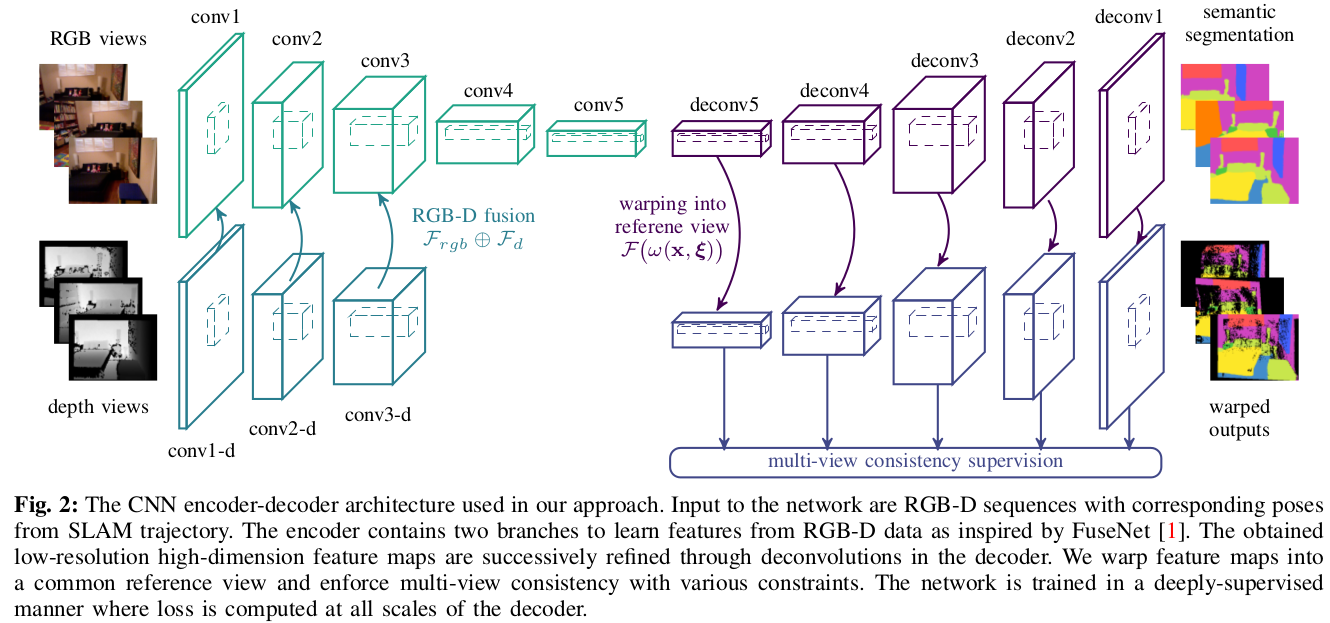
\includegraphics[width=0.95\textwidth]{SemanticSLAM/MultiView0.png}
\caption{基于Encoder-Decoder CNN的语义分割示意图}
\label{MultiView0}
\end{figure}

需要注意到有一下几点:
\begin{itemize}
\item 使用Unpooling、Deconvolution等实现Decoder
\item 注意,RGB与Depth经过两个分离的分支提取特征,然后在多个尺度(Multi-scale!)进行融合!
\item 使用KL散度作为Loss Function :

\begin{displaymath}
L(\mathcal{W}) = - \frac{1}{N} \sum_{i}^{N}\sum_{j}^{K}\lfloor j = l_{gt} \rceil \log p_j (x_i, \mathcal{W} | \mathcal{I})
\end{displaymath}

\item 使用Deeply Supervised Learning method计算all Upsample Scales,注意,Gound Truth使用\textbf{Stochastic Pooling}这种正则化技术生成各个尺度下对应的Gound Truth
\end{itemize}

\subsection{Multi-View Consistent Learning and Prediction}

本文的主要贡献是,Explore the use of temporal multi-view consistency within RGB-D sequences for CNN training and prediction. 这是通过把多帧数据Warp到一个Common Reference View来实现。

\subsubsection{Multi-view Data Associate Through Warping}

为了保证时间一致性,引入了Warping Layers。

该Layer的操作原理是:
\begin{displaymath}
X^{\omega} = w(x, \xi) = \pi (T(\xi)\pi^{-1}(x, Z_i(x)))
\end{displaymath}
其中,$\omega$为Warping function, $T(\xi)$为SLAM得到的位姿$\xi$下的单应变换;$\pi$实现3D坐标与图像坐标之间的转换。$Z_i(x)$为图像$x$处的深度信息。

\subsubsection{Consistency Through Warp Augmentation}

把KeyframeWarp到Neighboring Frames。

\subsubsection{Consistency Through Bayesian Fusion}

\begin{align}
p(y|z^i) & = \frac{p(z_i|y, z^{i-1})p(y | z^{i-1})}{z_i|z^{i - 1}} \notag \\
         & = \beta_i p(z_i | y, z^{i-1}) p(y | z^{i-1}) \notag
\end{align}

其中,$z^i$为到达第$i$帧的所有Measurements。

上式也就是Recursive Bayesive Update.

\subsubsection{Consistency Through Multi-View Max-Pooling}

Bayesian Fusion是在Probability域内进行的,而这里作者还尝试了直接在Feature域内进行Fuse。

使用Multi-View max-pooling对Warp 的 Feature Map进行处理。

\subsection{Experiments}

使用NYUDv2数据集、DVO-SLAM框架。

使用Cubic Interpolation来对RGB图像进行降采样,利用Nearest-neighbor Interpolation来对Depth和Labelling数据进行降采样

使用SGD Moment训练,动量为0.9,同时有0.0005的Weight Decay。Learning Rate 被设置为0.001然后每30K次迭代就Decay by a factor of 0.9。

使用IOU来判断Segment的效果。

\subsection{总结}

We base our CNN design on FuseNet,a recently proposed CNN architecture in an encoder-decoder scheme for semantic segmentation of RGB-D images.

All multi-view consistency training approaches outperform single-view trained baselines. They are key to boosting segmentation performance when fusing network predictions from multiple view points during  testing.

In future work, we want to further investigate integration of our approach in a semantic SLAM system, for example, through coupling of pose tracking and SLAM with our semantic predictions.

所以,作者的意思是说现在还没有达到Semantic SLAM的水平,而实现的也就是只有Semantic Segmentation吗!?SLAM只是提供了必要的位姿估计,来帮助相邻帧之间的Warping?

\section[MaskFusion]{MaskFusion: Real-Time Recognition, Tracking, and Reconstruction of Multiple Moving Objects}

MaskFusion,看样子挺厉害的样子。

A real-time, object-aware, semantic And dynamic RGB-D SLAM.({\color{red} 为什么这几篇基于RGB-D数据的算法这么多呢!?所以,要发文章的话,可以选面向不同输入数据的一种方法!比如,双目的文章我还没有看到,虽然上篇是关于Multi-View的语义分割,但不涉及SLAM啊。看样子生成语义地图的结果应该会挺炫的。})

可以实现更有优势的Instance-level的Semantic Segmentation。利用VR应用来表明MaskFusion的独特优势:Instance-aware, Semantic and Dynamic。

\subsection{背景及相关工作}

把SLAM应用到AR(Augemented Reality)时,还有两个问题解决的不太理想:
\begin{itemize}
\item 现在的SLAM系统均假设环境是静态的,会主动忽略Moving Objects
\item 现在的SLAM系统得到的均是一些几何的地图,缺少语义信息。有一些尝试,如SLAM++, CNN-SLAM
\end{itemize}

本文提出的MaskFusion算法可以解决这两个问题,首先,可以从Object-level理解环境,在准确分割运动目标的同时,可以识别、检测、跟踪以及重建目标。

分割算法由两部分组成:
\begin{itemize}
\item Mask RCNN

提供多达80类的目标识别等。

\item A geometry-based segmentation algorithm

利用Depth以及Surface Normal等信息向Mask RCNN提供更精确的目标边缘分割。

\end{itemize}

上述算法的结果输入到本文的Dynamic SLAM框架中。

使用Instance-aware semantic segmentation比使用pixel-level semantic segmentation更好。{\bfseries 目标Mask更精确,并且可以把不同的object instance分配到同一object category}。

本文的作者又提到了现在SLAM所面临的另一个大问题:Dynamic的问题。作者提到,本文提出的算法在两个方面具有优势:
\begin{itemize}
\item 传统的Semantic SLAM尝试

相比于这些算法,本文的算法可以解决Dynamic Scene的问题。

\item 解决Dynamic SLAM的尝试

本文提出的算法具有Object-level Semantic的能力。

\end{itemize}

{\color{red} \textbf{评语}:所以总的来说,作者就是与那些Semantic Mapping的方法比Dynamic Scene的处理能力,与那些Dynamic Scene SLAM的方法比Semantic能力,在或者就是比速度。确实,前面的作者都只关注Static Scene, 现在看来,实际的SLAM中还需要解决Dynamic Scene(Moving Objects存在)的问题。}

\subsubsection{Dense RGB-D SLAM}

KinectFusion证明使用Truncated Signed Distance Function(TSDF)可以表示室内地图构建,此外,其它的工作也证明使用合适的数据结构也可以完成室外环境的地图构建。

Surfels: Surface Elements, 在Computer Graph中应用比较早。

Surfel类似于Point Cloud,不同的是,Surfel不仅包含Location信息,还包含Radius和Normal等,此外,不像Point Cloud下在切换Mapping与Tracking之间时的Overhead.且是高效存储的。

\subsubsection{Scene Segmentation \& Semantic Scene Segmentation}

单纯的Scene Segmentation可以提供精确的目标边界,但缺乏Semantic Information.

Semantic Scene Segmentation作者只提到了基于MRFs的方法。

\subsubsection{Semantic SLAM \& Dynamic SLAM}

Semantic SLAM中提到了CNN-SLAM, Semantic Fusion

{\color{red} \textbf{评语}: 但作者的意思是这些算法没有考虑Object instance level的语义分割,而只考虑点云层面的分割,如果真是这样的话,那么不就没多少意义了,当然对人来说可能很清楚,但对机器而言,必须考虑Object Instance level.好像,这两个算法中确实就是这样。}

存在两种方法可以处理Dynamic SLAM的问题,而不把Moving Object当做Outlier来处理:
\begin{itemize}
\item Deformable world is assumed and as-rigid-as-possible registration is performed
\item Object instances are identified and potentially tracked rigidly
\end{itemize}

上面两种方法都涉及要么Template- 要么是 descriptor-based methods

\subsection{System Design}

\subsubsection{System Overview}

\begin{figure}[!hbtp]
\centering
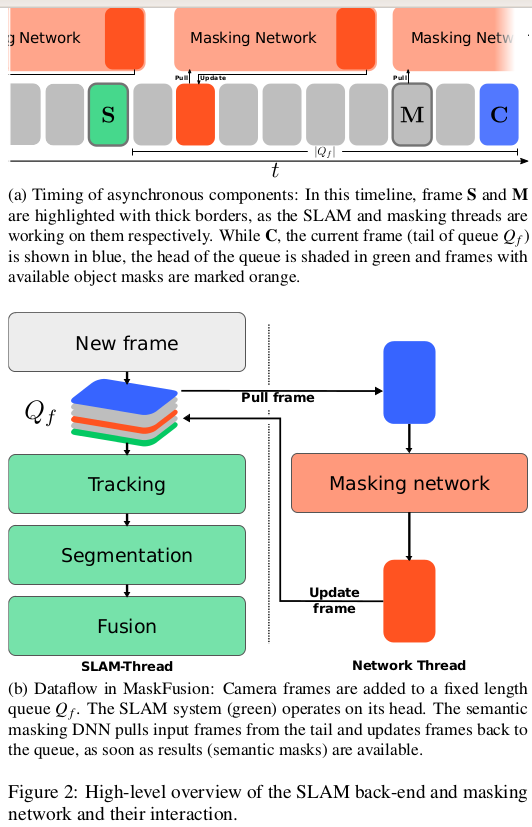
\includegraphics[width=0.85\textwidth]{SemanticSLAM/MaskFusion0.png}
\caption{Overview of MaskFusion}
\label{MaskFusion0}
\end{figure}

每新来一帧数据,整个算法包括以下几个流程:
\begin{enumerate}
\item Tracking

每一个Object的6 DoF通过最小化一个能量函数来确定,这个能量函数由两部分组成:几何的ICP Error, Photometric cost?。此外,作者仅对那些Non-static Model进行Track。最后,作者比较了两种确定Object是否运动的方法:
\begin{itemize}
\item Based on Motioin Incosistency
\item Treating objects which are being touched by a person as dynamic
\end{itemize}

\item Segmentation

使用了Mask RCNN和一个基于Depth Discontinuities and surface normals 的分割算法。前者有两个缺点:物体边界不精确、运行不实时。后者可以弥补这两个缺点, 但可能会Oversegment objects。

\item Fusion

就是把Object的几何结构与labels结合起来。

\end{enumerate}

\subsubsection{Multi-Object SLAM}

本文采用ElasticFusion类似的3D Model.其中,Model用Surfel来表示,Surfel具体包含以下内容:
$\mathcal{M}_m^s \in \{ \mathbf{p}\in\mathbb{R}^3, \mathbf{n}\in\mathbb{R}^3,\mathbf{c}\in\mathbb{N}^3,\mathbf{w}\in\mathbb{R},\mathbf{r}\in\mathbb{R}, \mathbf{t}\in\mathbb{R}^2  \}, \forall s < |\mathcal{M}_m|$, 分别表示:Position, normal, color, weiht, radius, and two timestamps.此外,系统还包含每一个目标的Label $l_m =m \forall m \in 0 \ldots N$, $N$是场景中包含的Object的数量。

这一步SLAM主要解决的问题是,对Ojbect的Pose的跟踪,由于输入时RGB-D数据,且像前面说的那样,作者的目标函数包含两个部分:
\begin{itemize}
\item Geometry Error

\begin{displaymath}
E_m^{icp} = \sum_{i}\left( (v^i - exp(\xi_m)v_t^i)\cdot n^i  \right)^2
\end{displaymath}

其中,$\xi_m$表示待求解的用6DoF李代数表示的相机位姿。$v^i, v_i^t$分别表示第$i$个vertex in surfels, 以及领一帧图像在这上面的投影。

\item Photoconsistency residuals

把输入的RGB图像转化成灰度图:$r, g, b \rightarrow 0.114r + 0.299g + 0.587b$, 然后这一部分的误差$E_m^{rgb}$参考论文。

\end{itemize}

总的目标函数就是两者之和:
\begin{displaymath}
E_m = \min_{\xi_m} \left( E_m^{icp} + E_m^{rgb} \right) 
\end{displaymath}

在完成Pose的跟踪后,然后跟下面的分割结果进行Associate。

这一步并不是每一帧都这样处理。

\subsubsection{Segmentation}

本部分主要包括三个小模块:
\begin{itemize}
\item Semantic Instance Segmentation

这部分就是Mask RCNN来做。

\item Geometric Segmentation

这一部分借鉴了别人的做法,在Depth图中引入两个概念:$\Phi_d$ Depth Discontinuity term, Concavity term $\Phi_c$, 然后如果$\Phi_d + \Phi_c > \tau$那么该点就是位于一个边缘上,是分割点。$\tau$是一个阈值。$\Phi_c, \Phi_d$在邻域上计算。

更多细节,看论文。

这一步是每一帧都会这样处理。

\item 如何把上面两个分割结果整合到一起,然后在与Map整合到一起

第一步与第二步并不是完全一致的,如果match了,才会整合到一起,平时用第二步比较多。

\begin{itemize}
\item Mapping geometric segmentation to Mask

根据Maximal Overlap进行匹配。

\item Mapping Mask to Model

\end{itemize}
\end{itemize}

\subsection{Evaluation}

使用了ATE、RPE、RMSE等评价指标。

\subsection{总结}

总的来说,本文算是一个大杂烩,亮点不是很明显啊,虽然在开始的地方,作者强调了几个本文解决的重要问题,但实际上,文中并没有看到清晰的对这些问题的解决。可能是我没看明白。

不过,在Geometry Segment这一块,作者借鉴了另一个工作,这与其它算法有点不同,其它的都是基于CNN的实现?输入是Depth数据,而作者这里没有用到CNN网络,而是通过一种邻域阈值的方法实现的。

另外一点就是,Tracking的时候,可能通过引入上面提到的两种不同的误差项就可以实现多目标跟踪吧,结果存疑,然后公式写的还那么非主流。

总体而言,并不好,前面的讨论倒是挺开拓视野的。


\section{小结 2}

现在看来语义SLAM主要的研究点:
\begin{itemize}
\item 输入数据:

单目、多目、RGB-D数据等,如果是单目等,可能就需要单独的SLAM框架来提供相机的Pose以及Depth, 如果提供了Depth可以考虑用CNN进行处理两种模式的数据。

\item 实时性

\item Semantic SLAM

现在要实现Object Instance-level,不能再是Point-level了,不然对于系统而言,可做的事情减少很多,因为只有认识Object Instance才能更好的交互,反而如果只有一堆Point的分类,对于机器系统用处不大吧,可能。

\item Dynamic SLAM

如何处理好Moving Object的问题。

\item 输出数据:

稠密还是稀疏?

\end{itemize}


\section[CNN-SLAM]{CNN-SLAM:}

{\color{red} 时间:2018.05.25}




\section{图像语义分割之FCN和CRF}

参考文章:\href{https://zhuanlan.zhihu.com/p/22308032}{图像分割2017.7-知乎}

知乎上专栏总结的一个总体分割框架:
\begin{figure}[!hbtp]
\centering
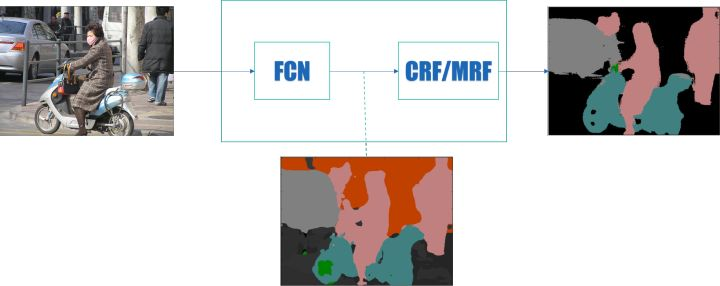
\includegraphics[width=0.85\textwidth]{SemanticSLAM/ImageSegmentFrame0.jpg}
\caption{图像分割的算法框架}
\label{ImageSegmentFrame0}
\end{figure}

前端使用FCN进行特征粗提取,后端使用CRF/MRF优化前端的输出,最后得到分割图。 

\subsection{前端FCN}

\subsubsection{FCN}

主要用到了三种技术:
\begin{enumerate}
\item 卷积化

卷积化即是将普通的分类网络,比如VGG16,ResNet50/101等网络丢弃全连接层,换上对应的卷积层即可。

\item 上采样

此处的上采样即是反卷积(Deconvolution)。当然关于这个名字不同框架不同,Caffe和Kera里叫Deconvolution,而tensorflow里叫conv\_transpose。CS231n这门课中说,叫conv\_transpose更为合适。

众所诸知,普通的池化(为什么这儿是普通的池化请看后文)会缩小图片的尺寸,比如VGG16 五次池化后图片被缩小了32倍。为了得到和原图等大的分割图,我们需要上采样/反卷积。

反卷积和卷积类似,都是相乘相加的运算。只不过后者是多对一,前者是一对多。而反卷积的前向和后向传播,只用颠倒卷积的前后向传播即可。所以无论优化还是后向传播算法都是没有问题。具体的原理,需要参考DLTips一章。

\item 跳跃结构

这个结构的作用就在于优化结果,因为如果将全卷积之后的结果直接上采样得到的结果是很粗糙的,所以作者将不同池化层的结果进行上采样之后来优化输出。

\end{enumerate}

\subsubsection{SegNet/DecovNet}

这两种结构可以直接参考原文,因为就只有结构的图示,没有详细解释。

\subsection{DeepLab}

首先这里我们将指出一个第一个结构FCN的粗糙之处:为了保证之后输出的尺寸不至于太小,FCN的作者在第一层直接对原图加了100的padding,可想而知,这会引入噪声。

而怎样才能保证输出的尺寸不会太小而又不会产生加100 padding这样的做法呢?可能有人会说减少池化层不就行了,这样理论上是可以的,但是这样直接就改变了原先可用的结构了,而且最重要的一点是就不能用以前的结构参数进行fine-tune了。所以,Deeplab这里使用了一个非常优雅的做法:将pooling的stride改为1,再加上 1 padding。这样池化后的图片尺寸并未减小,并且依然保留了池化整合特征的特性。 

但是,事情还没完。因为池化层变了,后面的卷积的感受野也对应的改变了,这样也不能进行fine-tune了。所以,Deeplab提出了一种新的卷积,带孔的卷积:Atrous Convolution.即图\ref{DeepLabAtrousConvolution0}所示。

\begin{figure}[!hbtp]
\centering
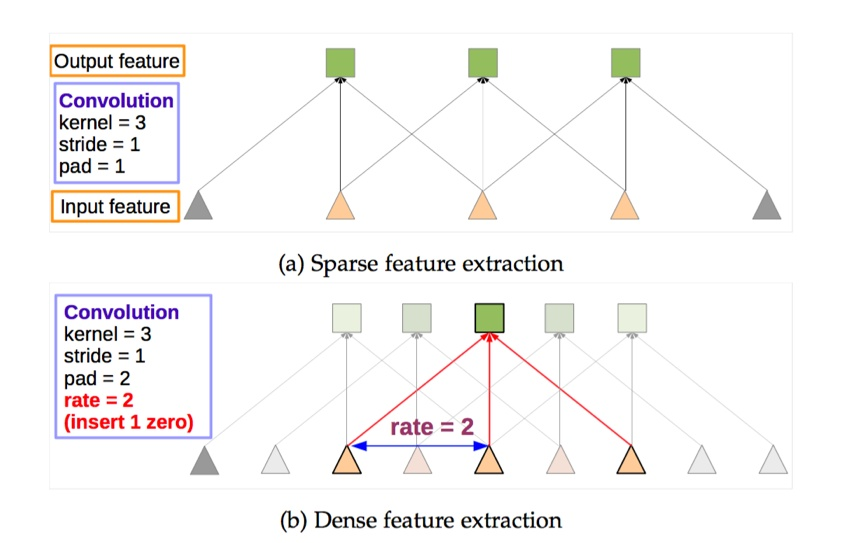
\includegraphics[width=0.75\textwidth]{SemanticSLAM/DeepLabAtrousConvolution0.jpg}
\caption{Atrous Convolution 示意图}
\label{DeepLabAtrousConvolution0}
\end{figure}

具体的感受野变化:

\begin{figure}[!hbtp]
\centering
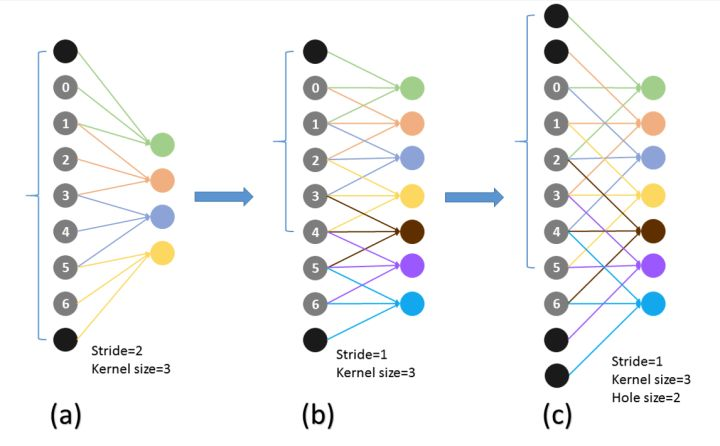
\includegraphics[width=0.85\textwidth]{SemanticSLAM/DeepLabAtrousConvolution1.jpg}
\caption{Atrous Convolution中的感受野变化 示意图}
\label{DeepLabAtrousConvolution1}
\end{figure}

图\ref{DeepLabAtrousConvolution1}中,a为普通的池化的结果,b为“优雅”池化的结果。我们设想在a上进行卷积核尺寸为3的普通卷积,则对应的感受野大小为7.而在b上进行同样的操作,对应的感受野变为了5(与a中颜色相同的输出所对应的输入只有0, 1, 2, 3 ,4。所以感受野变为5了。).感受野减小了。但是如果使用hole为1的Atrous Convolution则感受野依然为7.判断感受野的过程是,在输出数量一致的情况下(即和a中的输出的4种颜色相同的输出),所覆盖的输入的个数。

所以,Atrous Convolution能够保证这样的池化后的感受野不变,从而可以fine tune,同时也能保证输出的结果更加精细。

其实就是Dialted Convolution的思想。

\subsection{后端优化CRF/MRF}

\subsubsection{全连接CRF, DenseCRF}

对于每个像素$i$具有类别标签$x_i$还有对应的观测值$y_i$,这样每个像素点作为节点,像素与像素间的关系作为边,即构成了一个条件随机场。而且我们通过观测变量$y_i$来推测像素$i$对应的类别标签$x_i$。也就是说,这里的观察值$y_i$为对应第$i$位置的像素。

二元势函数就是描述像素点与像素点之间的关系,鼓励相似像素分配相同的标签,而相差较大的像素分配不同标签,而这个“距离”的定义与颜色值和实际相对距离有关。所以这样CRF能够使图片尽量在边界处分割。

在这里,势函数的输入来自FCN的输出。

而全连接条件随机场的不同就在于,二元势函数描述的是每一个像素与其他\textbf{所有}像素的关系,所以叫“全连接”。 

\subsubsection{CRFasRNN}

最开始使用DenseCRF是直接加在FCN的输出后面,可想这样是比较粗糙的。而且在深度学习中,我们都追求end-to-end的系统,所以CRFasRNN这篇文章将DenseCRF真正结合进了FCN中。

这篇文章也使用了平均场近似的方法,因为分解的每一步都是一些相乘相加的计算,和普通的加减(具体公式还是看论文吧),所以可以方便的把每一步描述成一层类似卷积的计算。这样即可结合进神经网络中,并且前后向传播也不存在问题。

当然,这里作者还将它进行了迭代,不同次数的迭代得到的结果优化程度也不同(一般取10以内的迭代次数),所以文章才说是as RNN。

\subsubsection{马尔科夫随机场, MRF}

没看懂,但还是把原文贴过来了。论文是:Deep Parsing Network

算了,还是去看论文吧,虽然我还没看。

\subsubsection{高斯条件随机场, G-CRF}

\subsection{小结}

2017.07.06

\begin{itemize}
\item FCN更像一种技巧。随着基本网络(如VGG, ResNet)性能的提升而不断进步。
\item 深度学习+概率图模型(PGM)是一种趋势。其实DL说白了就是进行特征提取,而PGM能够从数学理论很好的解释事物本质间的联系。 
\item 概率图模型的网络化。因为PGM通常不太方便加入DL的模型中,将PGM网络化后能够是PGM参数自学习,同时构成end-to-end的系统。

\end{itemize}

\section{Learning Deconvolution Network for Semantic}
参考文献:\href{https://zhuanlan.zhihu.com/p/26291607}{Learning Deconvolution Network for Semantic 1-知乎}

\href{https://zhuanlan.zhihu.com/p/27580384}{Learning Deconvoluton Network for Semantic 2-知乎}

背景:
FCN具有以下限制:
\begin{itemize}
\item 固定尺寸的感受野。对于对于大尺度目标,只能获得该目标的局部信息,该目标的一部分将被错误分类;对于小尺度目标,很容易被忽略或当成背景处理

\item 目标的细节结构容易丢失,边缘信息不够好。FCNs得到的label map过于粗糙,而用于上采样的反卷积操作过于简单

\end{itemize}

本文的主要贡献:
\begin{itemize}
\item 提出了可学习的反卷积网络, 并将其首次应用于语义分割
\item 分割结果是Instance-wise的分割,所以摆脱了原来FCNs中的尺度问题,这也是对应FCNs中的第一个问题
\item 在Pascal Voc12测试集上得到一个很好的效果,与FCN8s模型融合,得到当时最好的准确率
\end{itemize}

\begin{figure}[!hbtp]
\centering
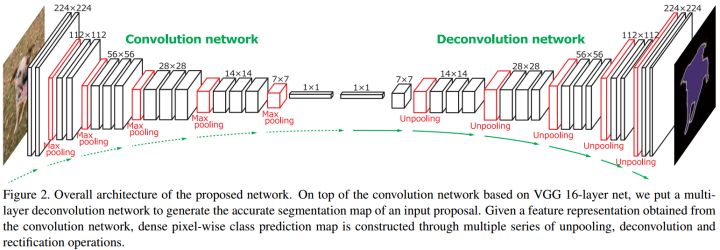
\includegraphics[width=0.95\textwidth]{SemanticSLAM/LearnDeconv0.jpg}
\caption{论文提出的神经网络结构}
\label{LearnDeconv0}
\end{figure}

反卷积网络主要由unpooling层、deconv层、relu层、BN层组成。

\subsubsection{Instance-wise Segmentation}

每张图片被裁剪为很多子图片,每张子图片包含一个目标实例。每张子图片作为输入,得到分割结果,再把这些分割结果聚合起来,得到整张图片的分割图。

\section[ReSeg 2015]{ReSeg: A RNN-based Model for Semantic Segmentation}

参考文献:\cite{ReSeg2015}

基于ReNet实现,每一层ReNet基于四个RNN实现,这四个RNN分别对应水平、垂直方向的双向信息。此外, ReNet is stacked在CNN之上,可以利用Generic local features。在ReNet之后,是提高分辨率的网络。

\subsection{背景 \& 相关工作}

普通的CNN会极大降低分辨率。FCN类的方法不能很好的利用local和global contextual dependencies, 而这些已被证明对分割具有较大帮助。因此,这些模型也经常利用CRF等作为后端处理,来locally smooth the model predictions, 但对于long-range contextual dependencies还是没有被很好的研究过。

而RNN可已被用于retrieve global spatial dependencies, 但是计算量较大。In this paper, we aim at the efficient application of Recurrent Neural Networks RNN to retrieve contextual information from images.

ReNet的每一层可以通过先水平扫描,然后垂直扫描来提高获取global information的能力。

在相关工作中,RNN可以实现分析长距离像素之间的关系,因此被用于语义分割中。ReNet具有很高的并行性,因为每一行之间的计算是相互独立的,每一列的处理也是独立并可以并行计算。

\subsection{Model Description}

首先,输入图像被送入在ImageNet上预训练好的VGG16网络。

然后,输出的Feature Maps被送进ReNet层,该结构可以sweep over输入的feature maps。

最后,多个Upsampling layer被用于把最后的Feature map的分辨率恢复到输入图像的分辨率的大小,接着,用Softmax进行分类。

使用GRU来很好的平衡存储量与计算能力的开销。

\subsubsection{Recurrent layer}

结构如图\ref{ReSeg0}所示。

\begin{figure}[!hbtp]
\centering
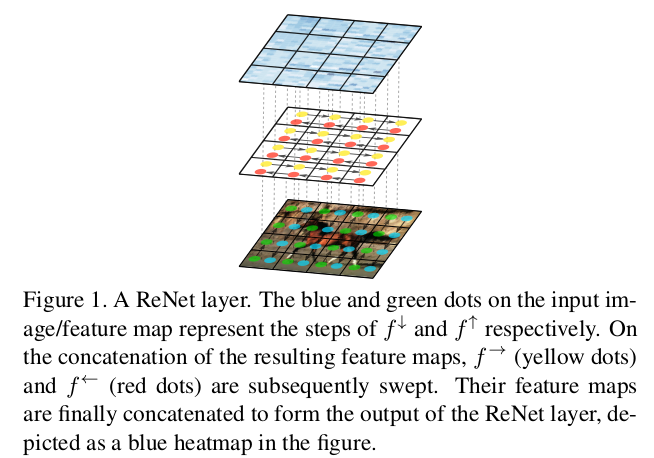
\includegraphics[width=0.75\textwidth]{SemanticSLAM/ReSeg0.png}
\caption{ReNet layer结构}
\label{ReSeg0}
\end{figure}

其中, $f^{\downarrow}$与$f^{\uparrow}$分别表示垂直方向两个方向的RNN, 具有U Recurrent unit结构?



\subsubsection{Upsampling layer}

作者说有三种提高分辨率的方法:
\begin{itemize}
\item Fully Connected layers

这种方法不适合,没有考虑输入的拓扑结构

\item Full convolutions

这种方法需要大的Kernel与Stride size等

\item Transposed Convolutions

这个方法好,既Memory efficient又Computation Efficient。

\end{itemize}

Transposed Convolution, 又被称为 Fractionally strided convolutions.下面是比较有意思的解释:
\begin{quote}
Convolution is based
on the observation that direct convolutions can be expressed
as a dot product between the flattened input and a sparse
matrix, whose non-zero elements are elements of the convolutional kernel. The equivalence with the convolution is
granted by the connectivity pattern defined by the matrix.

Transposed convolutions apply the transpose (转置) of this
transformation matrix to the input, resulting in an operation whose input and output shapes are inverted with respect to the original direct convolution.
\end{quote}

上一段的引用,详情可以从参考第八章中关于Deconvolution的说明,是一致的,且还有例子!

关于Deconvolution的更多说明可以参考:A guide to convolution arithmetic for deep learning.

\subsection{实验结果}

数据集:

Weizmann Horse, Oxford Flowers 17, CamVid Dataset.

使用IoU。

一个重要的现象:当数据集是Highly imbalanced, 分割效果会极大的变差, 因为此时网络会最大化那些经常出现的类别的分数, 而忽略不经常出现的类别?。为了解决这个问题,作者在Corss-entropy loss中加入了一个新的项,来bias the prediction towards the low-occurrence classes.

具体的就是:\textbf{Median Frequency Balancing}。

which re-weights the class predictions by the ratio between the median of the frequencies of the classes
(computed on the training set) and the frequency of each class. This increases the score of the low frequency classes (see Table 4) at the price of a more noisy segmentation mask, as the probability of the underrepresented classes is overestimated and can lead to an increase in misclassified pixels in the output segmentation mask.

\subsection{总结}

The proposed architecture shows state-of-the-art performances on
CamVid, a widely used dataset for urban scene semantic
segmentation, as well as on the much smaller Oxford Flowers dataset. We also report state-of-the-art performances on the Weizmann Horses.

\section[U-Net]{U-Net: CNN for Biomedical Image Segmentation}

参考文献:\cite{U-Net2015}

本文的一大贡献:证明通过更好的使用数据增广来提高现有训练数据的利用率。

另一大贡献,是提出一种结构,该结构由Contracting和Expanding两个部分组成,这一点与FlowNet类似啊。	

结果表明,仅需要非常少的图像数据就可以实现不错的效果。

\subsection{Network Architecture}

本文提出的网络结构实在FCN基础上进行的改进。

网络结构如图\ref{U-Net0}所示。

\begin{figure}[!hbtp]
\centering
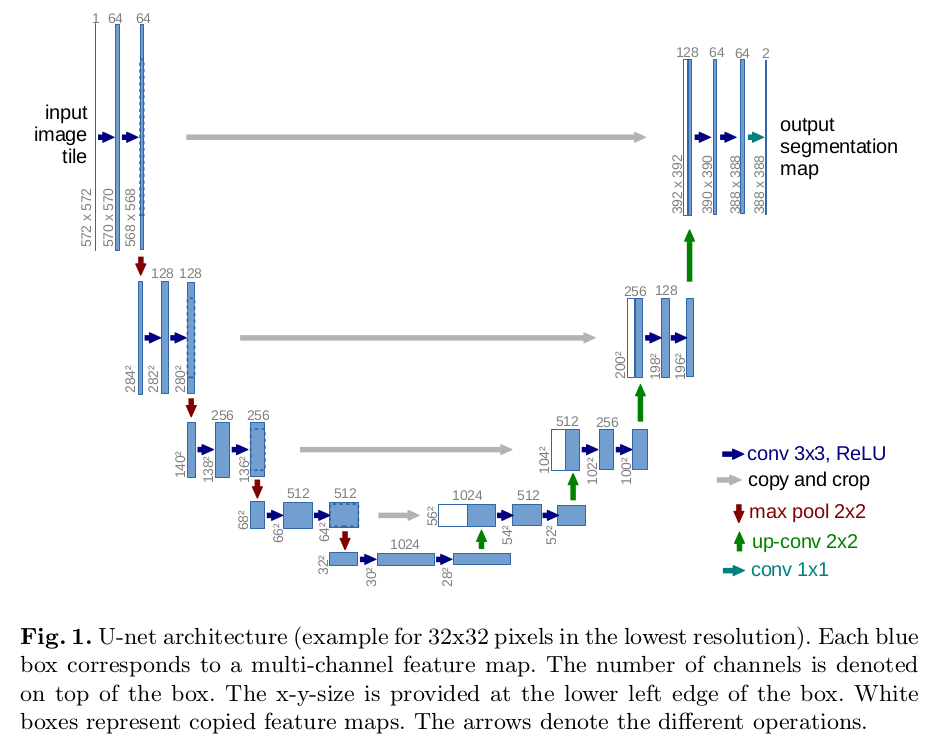
\includegraphics[width=0.8\textwidth]{SemanticSLAM/U-Net0.png}
\caption{U-Net结构示意图}
\label{U-Net0}
\end{figure}

与FCN不同的是,U-Net把结构分成Contracting与Expanding两个Path, Contracting部分与普通的卷及网络相同。It consists of the repeated
application of two 3x3 convolutions (unpadded convolutions), each followed by
a rectified linear unit (ReLU) and a 2x2 max pooling operation with stride 2
for downsampling. At each downsampling step we double the number of feature
channels.

而Expanding部分与FCN中不同的在于,其Feature Channel特别多,与Contracting中基本对称的一样多。每一层包含一个'Up-Convolution', 同时把Feature Channel数量减半。

在最后一层,一个1 * 1 的Convolution被用于把64-Component feature vector映射到目标的number of classes。

Contracting部分的Feature Map与Expanding Path部分的Feature Map会进行\textbf{Concatenation}, 这一点与FCN也不同。U-Net是在Channel维度进行拼接,而FCN是逐点相加!参考文章:\href{https://zhuanlan.zhihu.com/p/31428783}{FCN/U-Net结构解析-知乎}, 这一点属于特征融合步骤的不同!

在训练过程中,用到了Cross Entropy作为目标函数,同时进行数据增广:Shift, Rotation, Deformation, Gray value variantions.

貌似Random elastic deformation对于训练少量Label的数据来说非常重要。We generate smooth
deformations using random displacement vectors on a coarse 3 by 3 grid. The
displacements are sampled from a Gaussian distribution with 10 pixels standard
deviation. Per-pixel displacements are then computed using bicubic interpola-
tion. Drop-out layers at the end of the contracting path perform further implicit
data augmentation.


\subsection{Conclusion}

Thanks to data augmentation with elastic deformations (弹性变形), it only needs very few annotated images and has a very reasonable training time of only 10 hours on a NVidia Titan GPU (6 GB).

\subsection{补充}
\begin{itemize}
\item U-Net中的'Up-Convolution'是什么意思?

知乎上有文章说,就是用的Deconv来实现的。

\item 在最后的几层,如何把Feature map映射成语义分割图像呢?这在FCN\cite{Fcn2014}中也是之前被忽略的问题。

其实在最后的输出层也是一个Feature map, 它的Channel数量就是目标类别的数量,比如,在在Pacal中类别数为21(包括Background), 所以输出的最后的Feature Map具有21个Channel,这个可以参考FCN论文中的图1.另外,在图\ref{U-Net0}中也可以看出,最后的输出通道数为2,即每一类别代表一个channel,然后利用SoftMax进行在Channel维度上进行计算,得到对应像素的类别结果。这一步一般通过一个1*1的Convolution来实现。这一点也可以参考下面FCN论文中的原话:
\begin{quote}
	We append a 1 × 1 convolution with chan-
	nel dimension 21 to predict scores for each of the PAS-
	CAL classes (including background) at each of the coarse
	output locations, followed by a deconvolution layer to bi-
	linearly upsample the coarse outputs to pixel-dense outputs
	as described in Section 3.3.
\end{quote}

这么说来,原来Fully Convolution是这个意思,即相当于在原来Fully Connect的层在空间维度上进行扩充扩充,最终的结果是,现在每一个像素位置都对应于一个原来Fully Connect的维度的Vector!
\end{itemize}

总结一下, CNN图像分割基本上套路是:
\begin{itemize}
\item 下采样 + 上采样: Convolution + Deconvolution /Resize
\item 多尺度特征特征融合:如Concatenate或者逐点相加
\item 获得像素级的Segment Map, 一般通过n * 1*1 Convolution得到,其中$n$为类别数目。
\end{itemize}

\section{Semantic Visual Localization}

参考文献: \cite{SemanticVisualLocalization2017}
妹的,21页。

看样子,本文的主要主要关注点在于建立:Robust visual localization under a wide range of viewing condition.

本文提出利用使用联合\textbf{3D Geometry }和 \textbf{Semantic understanding of the world} 来帮助解决这个问题。

提出的算法, 利用一个新提出的生成模型来完成descriptor learning, 该过程trained on semantic scene completion as an auxiliary task.

最终,得到的3D descriptors可以很鲁棒,可以借助高层的3D geometric 以及 语义信息来处理丢失Observe的情况。

看样子,本文算法比较新颖,效果也很好,一个比较大的优势是采用了生成模型,而不是常用的判别模型。

\subsection{背景 \& 相关工作}

其实这篇文章主要的关注点是Localization, 也就是新的传感器数据来了后,怎么更加准确的与地图中的信息进行匹配,难点在于:The main challenge in this setting is successful data association between the query and the database.

为什么难呢,因为实际的场景是经常变化的,所以很容易就匹配错误了。一般的做法是基于描述子之间的匹配来定位,且通过提高描述子的质量来提高定位的质量。这种方法还是不好,比如尺度性不好、需要大量的匹配计算等。

本文提出了一种高效的描述子学习算法, 是基于生成模型而不是判别模型实现的。本文证明了,通过引入Semantics提供了strong cues 对于场景补全。而且不需要人为操作,就可以泛化到其它数据集以及其它传感器类型,并且都不需要重新训练!(生成模型这么强么还是本文的算法很强?)

生成的是3D 描述子。需要解决的一个重要问题是物体遮挡的场景(Occlusion),本文提出的算法通过借助Semantic Completion这一辅助任务来实现遮挡问题的解决。

本文的算法本质上还是提高Descriptor的生成质量以及匹配速度,在Euclidean space内完成。效果来看,可以在不同光照、季节变换等场景下实现定位。

优点没看明白。在相关工作中,作者分析了大量的已有的算法的缺点,我记得的主要的缺点就是:生成的Descriptor不鲁棒或不满足要求、匹配过程复杂、对多变场景处理不好等等。

\subsection{Semantic Visual Localization}

从上文可以看出,作者的主要贡献是:在Eculidean生成包含语义的3D Descriptor, 可以满足场景的多变、快速匹配、很高的精确度等需求。 

模型的输入数据:1) A set of color images with associated depth maps, 2) database image, including their respective camera poses.

算法过程:
\begin{enumerate}
\item 对于Database的一个子set, 预先生成其语义地图:$M_D$
\item 对于Query的一张或多张图像生成其语义地图$M_Q$
\item 建立$M_D$与$M_Q$之间的匹配,得到相机的位姿估计$\mathcal{P}_Q$
\end{enumerate}

上述算法过程,得到的结果,作者认为就可以实现对Extreme viewpoint和光照的鲁棒了。Semantic information is
comparatively invariant to these types of transformations through higher-level scene abstraction.

额,貌似走着不是对输入的RGB图像进行提取Descriptor, 而是对Semantic Maps提取Descriptors!这也行么?

按照上面三个步骤,具体内容如下:
\begin{itemize}
\item Semantic Segmentation and Fusion

首先生成所有输入图像的Dense pixelwise semantic segmentation, 然后把这些分割结果融合到\textbf{3D} Voxel maps $M_D$与$M_Q$。 

任务的目的是计算把Query 和 database map之间最佳匹配的位姿$P \in SE(3)$。

下面给出如何在缺少观察的情况下,通过对场景的语义理解来建立鲁棒的Semantic Maps。

\item Generative Descriptor Learning

又强调了一次:Semantic scene understanding is key to learning such an invariant function.

传统方案中, 有两种方式提高这种Invariant, 一种是学习更好的Matching function, 一种是学一种更好的Embedding。前者效果较好,但计算量很大,因为要比较每一对的Descriptor, 后者计算量小,本文的算法只需要每一个Descriptor计算一次就好。

具体使用一个Encoder来对Scene Semantics 和 Geometry进行编码。为了可以推理出没观察到的部分,算法还涉及一个Semantic scene completion的辅助任务, 同时推理Scenen Semantic 和 Geometry。整个结构如图\ref{SemanticVisualLoc0}所示:
\begin{figure}[!hbtp]
\centering
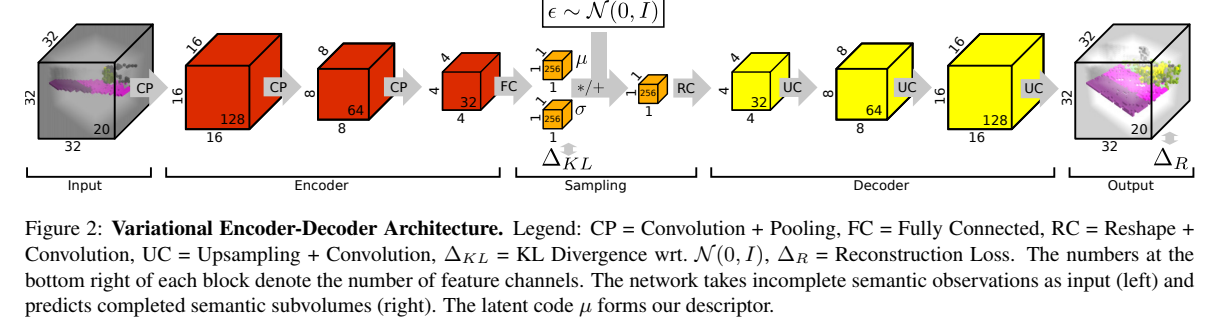
\includegraphics[width=0.85\textwidth]{SemanticSLAM/SemanticVisualLoc0.png}
\caption{Generative Descriptor Learning的示意图}
\label{SemanticVisualLoc0}
\end{figure}

\item Bags of Semantic Words

 Note that given an incomplete map, the bag of semantic words is a description of its complete
semantic scene layout. Our localization pipeline uses this representation to robustly match the query map to the database map, as detailed in the following.

这个bag of semantic words是通过计算属于$M$的所有subvolume来得到集合。也就是Encoder部分的输出构成的集合,具体得看论文吧。

\item Semantic Vocabulary for Indexing and Search

基于Euclidean metric来计算Query和Database之间的相似性,具体是利用Encoder部分的输出来计算距离。

\item Semantic Alignment and Verification

计算一组Query在不同Rotation下与Database之间的相似性,这些计算结果作为准确定位的基础,这就是这一小节要说明的内容。

通过类似于一种重投影误差的方式来判断计算的位姿的效果的好坏。

\end{itemize}

\subsection{Experiments}

用到了KITTI, NCLT数据集。

重复的场景结构容易引入Local Ambiguities, 会导致错误的定位。Global Ambiguities发生的较少,但会导致上百米的定位错误。通过考虑多帧的数据可以有效降低上述两种Ambiguities。此外,可以增加训练数据的多样性对于提高精度或许也有帮助。

\subsection{Conclusions}

In this paper, we proposed a novel method for localization using a joint semantic and geometric  understanding of the 3D world.

At its core lies a novel approach to learning robust 3D semantic descriptors. 

\section{小结3}

在前面两个小结的基础上,这里在强调一下几个重要的改进点!:

{\color{red} \bfseries 首先,实验目的是什么,有一些是实现Semantic SLAM, 也有提高定位信息的!然后,输入数据是什么, 现在趋势是借助多模态的数据,最经常用的是 Depth和RGB图像,此外,还有前面涉及到的Contour以及Semantic Information 和 3D Geometry信息,还有就是多帧数据实现非监督什么的。所以,一个可选的工作是,怎么把这些数据最高效的整合起来,可以借助RNN中的Gate思想,也可以看一下Knowledge 蒸馏法,以及Attention机制什么的!!!}

\section[StaticFusion]{StaticFusion: Background reconstruction for dense RGBD SLAM Dynamic Environments}

参考文献:\cite{scona2018staticfusion}

主要目的:提出一个鲁棒的、稠密的、基于RDBD的、可处理Dynamic Environment的 SLAM系统。

可以实现对Static和Dynamic Environment的分割,以及只对Static部分建模,来提高相机位姿估计的精度,降低overal drift的影响。

\subsection{背景}

现有的SLAM系统都假设场景是静态的,所以通过图像对之间的匹配可以得到相机的变换关系。但是现在场景中存在动态目标,那么图像之间的匹配就不单单是由于相机变换引起的了,所以需要区分静态场景和动态场景,并且动态场景对地图的构建也会产生不可逆的影响。

主要做了两件事:
\begin{itemize}
\item 同时估计相机的位姿以及对static和Dynamic场景的分割

其中,RGBD相机估计,通过把新来的图像帧与一个稠密的surfel-based SLAM model一起实现,如ElasticFusion。

\item 使用Static场景对环境进行了更具有一致性的建模
\end{itemize}

作者有公开源码。

\subsection{动态场景下SLAM系统的相关工作}

ElasticFusion是首个基于RGBD的SLAM系统,现在在Scalable estnesion、loop clusure capabilities、consider run-time limitations等方面改进,这一小节主要总结在Dynamic Environment场景下的一些改进方法。主要有三个方面:
\begin{itemize}
\item Implicit Handing of Dynamic Elements

这一类算法通过对High-residual points施加惩罚项来提高位姿估计的鲁棒性。其他的如ElasticFusion等算法在构建地图之前,需要目标在连续的多帧图像中都可以观察到,才会被认为是Static部分,加入到地图构建中。但这些算法并不会明确的对Dynamic Object进行处理,只能适用于运动物体在图像中范围比较小或者相机的运动幅度很小。

\item Outlier Rejection Strategies

一种常用的方法是把Dynamic moving object当做噪声来处理,被检测出来然后被滤波去除。

这一类的方法包括:DTAM、ORB-SLAM等。通过非常保守的关键帧选取策略来提高系统的鲁棒性。但这些算法并没有考虑在连续帧中检测Dynamic points是使用Spatial和temporal上面的Coherence。

{\color{red} \textbf{评语}:所以在Temporal上的Coherence可以使用RNN来帮助解决,而在Spatial上面的Coherence可以通过CRF之类的算法实现,最近不是也有ConvCRF的算法出现么!可以考虑考虑。}

\item Methods Enforcing Spatial on temporal Coherence

此外,还可以借助IMU以及Robot's odometry来提高Dynamic下的SLAM的鲁棒性,但本文主要基于单目RGBD相机来做。

\end{itemize}

\subsection{Framework和Notation}

主要的流程:
\begin{figure}[!hbtp]
\centering
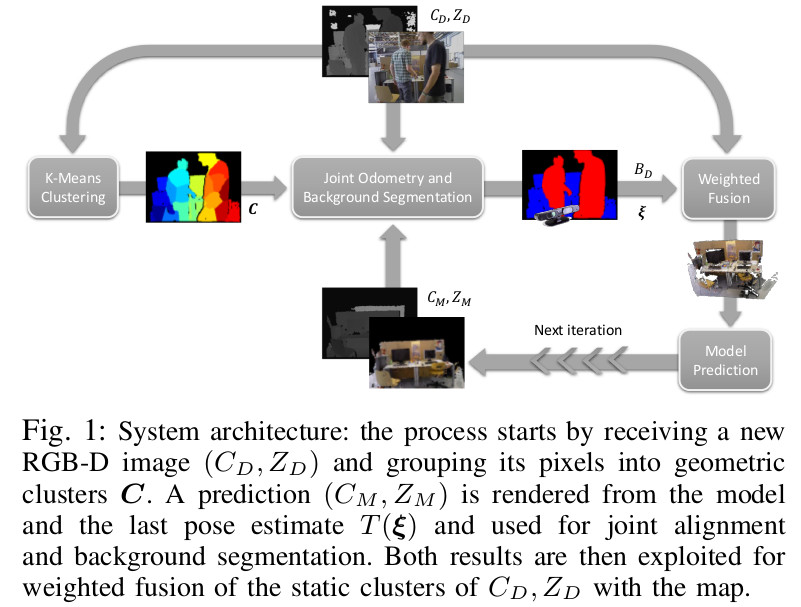
\includegraphics[width=0.75\textwidth]{SemanticSLAM/StaticFusion0.png}
\caption{StaticFusion算法的三个主要流程}
\label{StaticFusion0}
\end{figure}

三个步骤:
\begin{enumerate}
\item From incoming pair $I_D, Z_D$ 得到3D Geometry Cluters $\mathbf{C}$

其中, $C_D$是输入的彩色图像, $Z_D$是输入的Depth图像, $I_D$是基于$C_D$得到的Intensity image。这个分割算法来自于:Fast odometry and scene flow from RGB-D cameras based on geometric clustering.作者假设分割后的每一个cluster是rigid body.

\item 根据上一帧的相机位姿预测这一时刻的场景图片$C_M, D_M$, 然后这个预测结果与这一时刻实际的数据的分割结果来联合估计相机的运动$\xi \in \mathfrak{se}(3)$, 与此同时,这一步还会得到一个基于运动的场景分割,对于每一Cluster,我们分配一个Score, $b_i \in [0, 1]$, 来表示这一个Cluster属于Dynamic还是Static, 本文中,$b_i = 1$是Static, $b_i=0$是Dynamic, 在之间则表明不同程度的不确定性。

具体还会用到到上一时刻截止的Map信息。

\item 最后,利用上一步计算得到的$\xi$和运动分割结果, 得到一个pixel-wise的分割图\ref{StaticFusion0}中的$B_D$, 这一步只处理输入上一步计算的Static部分来计算。然后这个计算结果与输入$C_D, Z_D$进行加权\textbf{3D} Fusion。

\end{enumerate}

每一步的具体实现,还需要下面的讲解。

\subsubsection{第二步的计算}







\section{Convolutional CRFs for Semantic Segmentation}

参考文献:\cite{marvin2018crf}

之前的研究人员会用CRF作为语义分割的后处理步骤,但CRF有两个缺点:训练困难,推理计算速度慢。

为了解决这两个问题,作者在本文中提出在全连接CRF中引入条件独立性的假设。这样的后果就是,我们可以以卷积的形式重新组织CRF的推理计算过程,而且可以通过后向传播的方式在训练过程中优化模型参数。最终可以借助GPU进行加速训练,效果是速度可以提高两个数量级。

\subsection{背景 \& 相关工作}

传统用于语义分割的CNN的缺点是:只能提取局部特征,不能利用全局的Contexture。所以有人认为简单的前向CNN不能满足Structured Predictions类任务。

在FCN的基础上,Transposed convolution layer用于提高Feature Map的分辨率,Dilated convolutions用于提取空间信息(Spatial information)。很多网络结构都是基于这种思路来做的!而这一类做法严重依赖于CNN提取特征的能力,进行pixel-wise的预测。stuctured knowledge and background context被忽略。

一种在CNN中加入sturctured predictions into CNN的方法是在CNN的输出上加入fully-conneced CRF进行后续处理。Pyramid pooling是另一种与CRF类似作用的方法, 用于提高CNN的感受野,但并不会提供真正的structured reasoning。

还是那句话,主要是两个问题,那么现在有哪些方法来解决这两个问题呢?
\begin{itemize}
\item Parameter Learning in CRFs

一些方法包括:EM和Grid-search, Gradient Decent, Quadratic Optimization等。但都不太适合CNN的训练流程。

\item Inference speed of CRFs

一些方法输出降维的数据,但会影响预测能力。据作者所知,目前还没有一种可以有效提高FullCRFs推理速度的方法。

\end{itemize}

\subsection{Fully Connected CRFs}

CRF嘛,基于随机场的原理来实现的。首先说明下符号:$I$是输入图像,具有$\mathbf{n}$个像素;$\mathbf{X}\in \{ X_1, \ldots, X_n \}$表示每一个像素的标签,即分割结果中的类别;假设共有$k$个类别,即每一个$X_i$都有$k$个可能的取值。所以得到的条件随机场模型,以吉布斯分布的形式(基于成本函数表示的吧应该):
\begin{displaymath}
P(X=\hat{x}|\tilde{I}=I) = \frac{1}{Z(I)}\exp(-E(\hat{x}|I))
\end{displaymath}

其中,$E(\hat{x}|I)$表示能量函数,由下式给出:
\begin{displaymath}
E(\hat{x}|I) = \sum_{i \le N}\psi_u(\hat{x}_i|I) + \sum_{i\ne j \le N}\psi(\hat{x}_i, \hat{x}_j | I)
\end{displaymath}

上式中的第一项是Unary Potential,传统的来自于普通的CNN的语义分割结果可以认为就是这一项的具体取值了。那么还有后一项,后一项包含两个像素的分割结果,表示的就是利用Spatial Information了。重点说一下这一项。

后一项叫做Pairwise Potential,表示$\hat{x}_i, \hat{x}_j$的联合分布,这里的$x_i, x_j$其实也是可以是来自于CNN的语义分割预测结果,与Unary potential中的输入是一样的!可以用于明确表示这两个像素之间的联系,如近似的颜色等。在FullCRFs中,这一项是基于weighted sum of M个 gaussian kernels来实现的。
\begin{displaymath}
\psi(x_i, x_j | I) = \mu(x_i, x_j)\sum_{m=1}^{M}\omega^{(m)}k_G^{(m)}\left( f_i^I, f_j^I \right)
\end{displaymath}

其中,$\omega^{(m)}$是可以学习的参数,特征向量$f_i^I, f_j^I$可以任意选择,并可以依赖于输入图像$I$。但是最开始的那个函数$\mu(x_i, x_j)$是the compatibility transformation,只与$x_i, x_j$有关,而与输入无关。接下来重点说一下这个函数的选择。

一种普遍的选择是用Patts Model来做$\mu(x_i, x_j) = |x_i \ne x_j |$,关于这个模型,可以参考Wikipedia,我记得笔记中也有,但记不清了。而在CRFasRNN中,提出利用1*1的卷积来做Compatibility transformation。这样一种函数可以让模型学习更多的structured interactions between predictions。

说完了$\mu$函数,那么来看一下在FullCRF中,是怎么实现后面对Gaussian kernel的加权的吧。在FullCRF中,有两个Gaussian Kernelz作为hand-crafted features。Appearance kernel $k_\alpha$考虑了颜色的取值$I_i, I_j$作为特征; smoothness kernel基于spatial corrdinates$p_i, p_j$来实现。整个的Pairwise potential 由下式给出:
\begin{displaymath} 
k(f_i^I, f_j^I) = \omega^{(1)}\exp\left( -\frac{|p_i - p_j|^2}{2\theta_\alpha^2} -\frac{|I_i - I_j|^2}{2\theta_\beta^2} \right) + \omega^{(2)}\exp\left( -\frac{|p_i - p_j|^2}{2\theta_\gamma^2} \right)
\end{displaymath}

其中, $\omega, \theta$都是可以学习的参数。需要指出的是,这是一种Hand-crafted feature,有助于提高CRF的优化效率。

\subsubsection{Full CRF的Mean field inference}

FullCRF的推理主要基于Mean Field inference来实现的。具体步骤如图\ref{ConvCRF0}所示。

\begin{figure}[!hbtp]
\centering
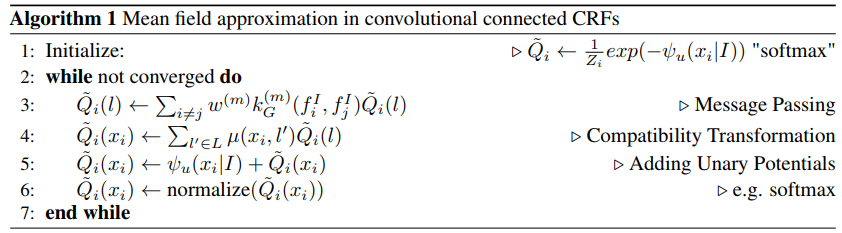
\includegraphics[width=0.85\textwidth]{SemanticSLAM/ConvCRF0.png}
\caption{Mean field inference算法步骤}
\label{ConvCRF0}
\end{figure}


对这个算法,简单说两句,除了message passing这一步之外,其它的几个步骤都是可以高度并行的。可以用GPU进行加速。 Message Passing也是CRF计算的瓶颈,计算量与输入图像的像素数的平方成正比,有研究人员提出利用Permutohedral lattice模型来近似,从而提高计算效率,这个近似模型是一种高维的滤波算法。但这种模型是基于一种很复杂的数据结构来实现的,存在基于CPU的复杂但快速的实现,但不适合GPU的实现。实际上,Permutohedral lattice模型的梯度求解也是一件很麻烦的事情,这也是为什么FullCRF之类的算法基于Hand-crafted features来做。

\subsection{Convolutional CRFs}

Convolution CRF其实就是在Full CRF的基础上引入了条件独立假设,即如果两个特征之间的Manhattan距离超过一个阈值$k$即$d(i, j) > k$那么就认为这两个点之间是独立的,这个$k$作者称为filter-size。

在Pairwise Potentional上面的体现就是,若大于这个阈值,$\psi_p$为0。

\subsubsection{Efficient Message Passing in ConvCRFs }

上面也提到了,Message Passing是CRF的计算瓶颈,本文提出的方法可以有效解决这个瓶颈,这是本文的主要贡献之一, 就不需要再使用Permutohedral模型近似了,也可以借助GPU加速计算了。为了实现这个目标,作者提出利用截断Gaussian Kernel实现的卷积操作来完成Message Passing这一步,这样就可以利用普通的CNN来完成了。

假设输入$P$是的尺寸是$[bs, c, h, w]$, 分别对应Batch size、通道数、高度、宽度。最终可以得到下面的公式,具体的构成看论文吧,那个公式有点复杂。

\begin{displaymath}
Q[b, c, x, y] = \sum_{dx, dy \le k} K[b, dx, dy, x, y] \cdot P[b, c, x+dx, y+dy]
\end{displaymath}

可以看出滤波器的取值还与Spatial dimension有关,需要注意的地方是,卷及操作实在通道为度上进行的。{\bfseries 这里进行的信号处理中的卷及操作,而不是NN中的卷及操作,后者其实是相关操作。}

这一步可以基于GPU来加速,但会涉及GPU中数据的重新组织,而实际上90\%的GPU运算时间都花在了数据重新组织上了。有一段关于卷积运算的阐述看论文。

\subsubsection{Additional implementation details}

ConvCRF中的设计策略与FullCRF中相同,即使用Softmax进行归一化、使用Potts model以及Hand-crafted gaussian featreu等。同样的,对Pairwise kernels做Gaussian blur,这样可以增加滤波器的有效大小变成4倍,这是为什么!

作者也实现了基于1*1卷积的实现,作为实验结果进行分析, 或者在Pairwise 中的输入换成可以学习的Feature数值。

使用VOC2012。使用ResNet101作为Unary potentials。

训练的时候,采用Decoupled Training的策略。即首先训练CNN模型,以语义分割为目标;然后固定CNN的输出,进行CRF的训练。

{\color{red} \bfseries 评语: 可以看得出来,作者是用CNN输出的完整分辨率的CRF进行训练的,这得多耗时,所以,下一步就是在Feature领域进行CRF操作!}


\subsection{总结}

通过增加条件独立的假设,我们可以去除Permutohedral lattice approximation,从而可以借助GPU完成高效的消息传递的计算,并是以卷积的方式进行。

下面,作者说还是要如何更好的捕获全局信息。也会把ConvCRF应用于Instance Segmentation以及Landmark recognition等应用中看一下效果怎么样!




\section[Co-Fusion]{Co-Fusion: Real time segmentation tracking and fusion of multiple objects}

参考文献:\cite{runz2017co}

输入的数据是RGBD, 主要通过对运动物体进行建模,完成场景的描述,可以作用在动态场景下。

表现在:把场景分割成多个Objects, 并实时的对他们进行跟踪和Shape建模。


\section{Squeeze-and-Excitation Networks}

参考文献:\cite{senet2017hu}

本文主要的关注点是如何更好的处理Channel-wise的信息。普通的卷及操作,会同时考虑局部的区域特征以及不同特征图之间的组合,而本文主要考虑Channel wise信息的提取,作者认为这样可以提高模型的表示能力!

具体结构如下图所示:
\begin{figure}[!hbtp]
\centering
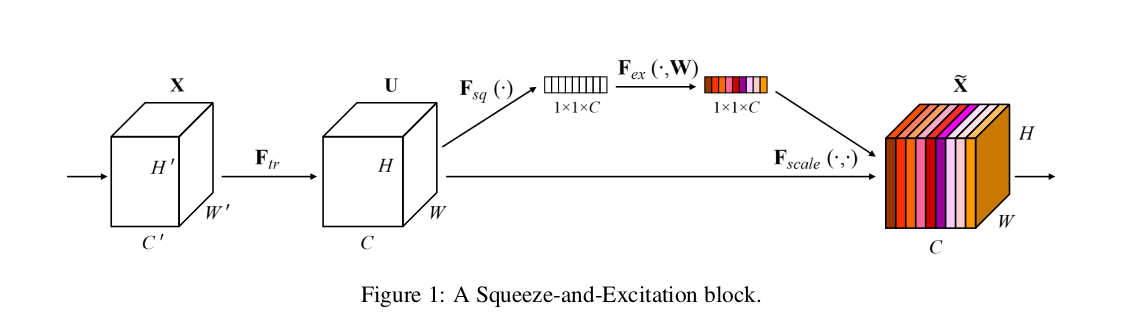
\includegraphics[width=0.85\textwidth]{SemanticSLAM/SENet0.png}
\caption{SENet结构示意图}
\label{SENet0}
\end{figure}

图\ref{SENet0}需要注意以下几点:
\begin{itemize}
\item $F_{sq}(\cdot)$表示文中所说的Sequeeze,这是基于Global Max Pooling (GAP)实现的,所以这一步并不会引入额外的参数,只又很少量的计算代价.这一步的结果就是输入的Feature Map编程$1 \times 1 \times C$的向量,作者把这个vector称为Channel Descriptor。
\item $F_{ex}(\cdot, \omega)$表示文中所说的Excitation,这是由Sigmoid和Bottleneck结构实现的。Bottleneck结构是两层具有不同输出维度的全连接层,可以表示成:
\begin{displaymath}
\mathbf{s} = F_{ex}(\mathbf{z}, \mathbf{W})=\sigma(g(\mathbf{z}, \mathbf{W})) = \sigma(\mathbf{W}_2 \sigma (\mathbf{W}_1 \mathbf{z}))
\end{displaymath}


其中$\sigma$为ReLU,$W_1 \in R^{\frac{C}{r}\times C}$, $W_2 \in R^{C \times \frac{C}{r}}$, 其中C表示输入Feature Map的通道数,也就是$\mathbf{U}$的通道数,这一结构也称为Bottleneck,是为了降低参数数量,r是ratio,作者实验证明了可以选择16。

\item $F_{scale}(\cdot, \cdot)$表示Channel-wise的相乘

\item 作者的实验表明,这个S-and-E Block放在网络结构的中部、前部比较好,放在后面效果不是特别很好,但会增加比较多的参数,因为后面的通道数C比较大,所以可以去掉。这是基于ResNet验证的。
\end{itemize}

如何把SE Block加入到ResNet等网络中,可以看文章。

\section{Deep Multi-scale Architectures For Monocular Depth Estimation}

参考文献:

本文主要回顾使用Multi-scale的网络结构进行深度估计,表明相比于只使用一种Scale的Feature,可以提高精度、定性上更好的深度图。在NYU Depth上实现了SOTA。

\subsection{背景与相关工作}

有学者指出,受人类视觉的激发,发展了一些算法,人类视觉会利用Texture, Perspective, defocus等信息。

最早的两篇基于深度学习来做的工作是:

\begin{itemize}
\item Deep Deconvolutional Networks for Scene Parsing
\item Depth map prediction from a single image using a multi-scale deep network
\end{itemize}

基于这两个工作,后面提出了非常多的改进方法,但比较少关注多尺度问题。本文的实验表明,如果在小的数据集上,多尺度网络可以比精心设计的单尺度网络更好一点的话,那么在打的数据集上,就会有SOTA结果。

相关工作有:
\begin{itemize}
\item Depth map prediction from a single image using a multi-scale deep network, 2014

网络结构包含两个部分,由两个网络Stack而成。第一个网络输出Coarse depth map, 第二个网络对输出的这个粗糙的深度图进行Refines, 后一个网络通过3 successive卷积实现,用Coarse depth map和RGB image作为输入。

\item Predicting depth, surface normals and semantic labels with a common multi-scale convolutional architecture. 2015

增加了一个新的CNN模块,同时多任务预测。

\item Towards unified depth and semantic prediction from a single image, 2015

使用语义信息帮助深度估计。

\item Learning depth from single monocular image using deep convolutional neural fields, 2016

\item Deep convolution neural fields for depth estimation from a single image, 2015

\item Depth and surface normal estimation from monocular images using regression on deep features and hierarchical crfs. 2015

\item Monocular depth estimation using neural regression forest. 2015

\item Depth from a single image by harmonizing overcomplete local network predictions, 2016

\item Deeper depth prediction with fully convolutional residual network, 2016

Encoder-decoder network。 实验表明使用BerHu loss可以提高精度。是下了SOTA的实验结果。

\end{itemize}


\section{Depth Map Prediction from a single image usign a multi-Scale Deep Network}

参考文献:

基于单目图像预测深度需要来自于多个Cues的both global and local信息。本文的两个主要贡献:
\begin{itemize}
\item 提出利用two network stack完成深度预测,一个完成coarse global prediction based on entire image, 另一个完成refines this prediction locally.
\item 提出一个scale-invariant error,帮助测量深度
\end{itemize}

整体结构如图\ref{DepthPrediction2014_0}所示:
\begin{figure}[!hbtp]
\centering
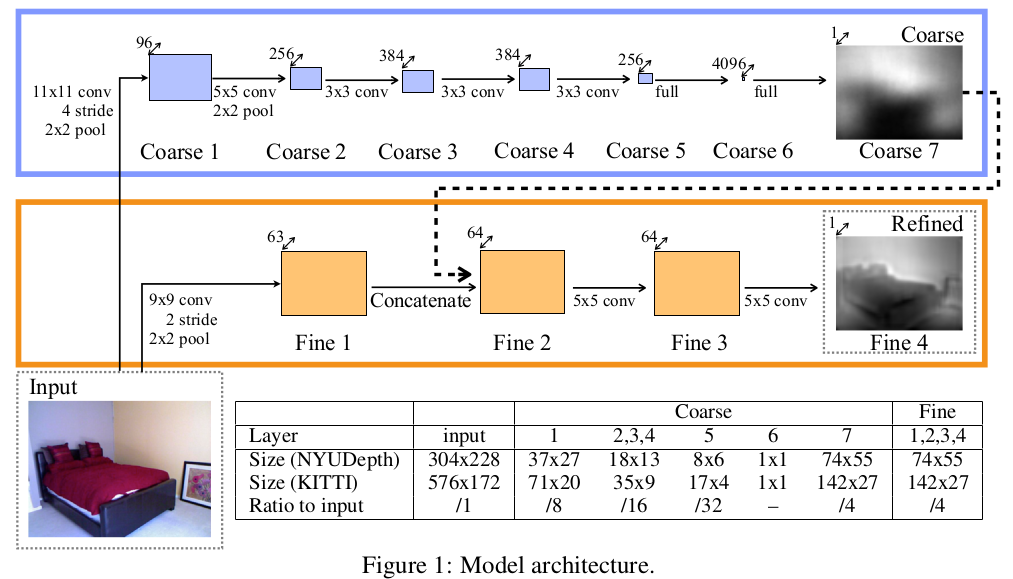
\includegraphics[width=0.85\textwidth]{SemanticSLAM/DepthPrediction2014_0.png}
\caption{网络结构示意图}
\label{DepthPrediction2014_0}
\end{figure}

在第一个部分,也就是得到Coarse Depth Map的部分,通过全连接层实现输入图像的全局视野,此外,在中间几层使用Max Pooling增加局部的感受野。但有一地方是如何根据Coarse6的输出得到Coarse7。作者也没说明白!全连接中还应用了Dropout。

在第二部分,首先对输入图像进行一次卷积运算,然后结果与上面的Coarse7的输出进行Concatenate,后面的卷积运算都会有Zero padding保持输出的大小一致。

第二个贡献是提出了一个Scale-Invariant Error (Metric), 因为单目预测深度的时候会有尺度问题,所以作者用下面的公式:
\begin{displaymath}
D(y, y^{*})  = \frac{1}{2n}\sum_{i=1}^{n} \left( \log y_i - \log y^{*}_i  \alpha(y, y^{*}) \right)^2
\end{displaymath}
其中,$ \alpha(y, y^{*})= \frac{i}{n}\sum_{i}(\log y_i - \log y^{*}_i)$.$n$为像素的个数,$i$为像素的索引。

最后作者的目标函数就是基于这个Scale-Invriant Error来做的。

\begin{displaymath}
See the paper.
\end{displaymath}

由于网络最后的输出是下采样了4倍,所以,在训练的时候需要把depth和mask都直接下采样比例为4。

\section{Mask R-CNN}

参考文献:

这篇文章的重要贡献是实现了Instance-Level的语义分割,具体是实现实在Faster-RCNN的基础上,新增了一个Branch用于预测Object Mask。它与物体检测(Object Detection)的区别是,提供Mask的预测结果而不是Boundingbox;它与语义分割的区别是,它是Instace-level的分割,而不是像素级的、不区分Instance的分割。

示意图如图所示:
\begin{figure}[!hbtp]
\centering
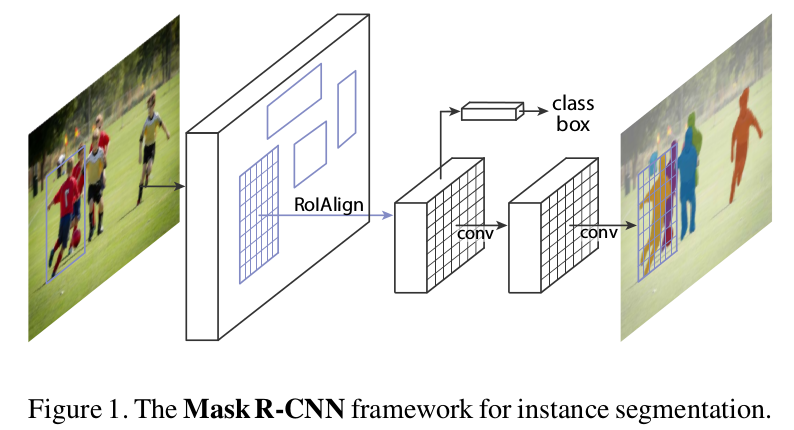
\includegraphics[width=0.85\textwidth]{SemanticSLAM/MaskRCNN0.png}
\caption{Mask RCNN示意图,在class box的基础上增加了预测mask的分支。}
\label{MaskRCNN0}
\end{figure}

\subsection{研究现状与相关背景}

在Faster-RCNN的基础上实现的,但是由于Faster-RCNN中的RoI Pooling会导致网络的输出与输入并不是Pixel-by-pixel的Alignment, 所以,在得到Mask的时候,作者提出利用RoIAlign的结构,可以faithfully preserves exact spatial locations.

{\bfseries 非常重要的一点是:mask和class 的预测是分离的(decouple)的两个过程,而FCN之类的算法是既需要perform per-pixel multi-class categorization, which couples segmentation and classification,后一种方式对Instance segmentation的效果较差。}


\subsection{Mask RCNN}


\subsection{实验}


\subsection{总结}





\subsection{常用数据集}

\subsection{KITTI}

数据集官网:\href{http://www.cvlibs.net/datasets/kitti/index.php}{KITTI Dataset}

参考文章:

[1] \href{https://blog.csdn.net/Solomon1558/article/details/70173223}{KITTI数据集简介和使用-CSDN}

KITTI数据集由德国卡尔斯鲁厄理工学院和丰田美国技术研究院联合创办,是目前国际上最大的自动驾驶场景下的计算机视觉算法评测数据集。该数据集用于评测立体图像(stereo),光流(optical flow),视觉测距(visual odometry),3D物体检测(object detection)和3D跟踪(tracking)等计算机视觉技术在车载环境下的性能。KITTI包含市区、乡村和高速公路等场景采集的真实图像数据,每张图像中最多达15辆车和30个行人,还有各种程度的遮挡与截断。整个数据集由389对立体图像和光流图,39.2 km视觉测距序列以及超过200k 3D标注物体的图像组成[1] ,以10Hz的频率采样及同步。总体上看,原始数据集被分类为’Road’, ’City’, ’Residential’, ’Campus’ 和 ’Person’。对于3D物体检测,label细分为car, van, truck, pedestrian, pedestrian(sitting), cyclist, tram以及misc组成。

\subsection{官网资源介绍}

最官网页面顶部,一共分了13栏,如图\ref{KITTI0}所示。

\begin{figure}[!hbtp]
\centering

\includegraphics[width=0.75\textwidth]{SemanticSLAM/KITTI0.png}
\caption{KITTI官网截图}
\label{KITTI0}
\end{figure}

其中,这些栏分别对应不同的应用目的提供单独的数据集,如Stereo, flow, sceneflow, depth, odometry, object, tracking, road, semantics, row data等。其中前三个貌似是对应同一个数据集。在depth中会有深度预测和深度补全等功能,semantics等包含一些标注好的图像数据等。Odometry等数据集比较大!

此外,作者还提供了一个Submit results栏,可以上传自己的测试结果等。但不能造假,即训练过程中,需要自己负责把训练数据分成train data 和 validate data, 然后用test data对模型进行测试。

\subsection{详述}

主要参考本小节的参考文章。

原始数据采集于2011年的5天,共有180GB数据。 

\subsubsection{组织形式}

图所示为早期的数据组织形式,与目前KITTI数据集官网公布的形式不同。在这早期的版本中,一个视频序列的所有的传感器数据都存储于data\_drive文件下, 其中data和driver是占位符,表示采集数据的日期和视频编号。时间戳记录在Timestamps.txt文件中。

\begin{figure}[!hbtp]
\centering
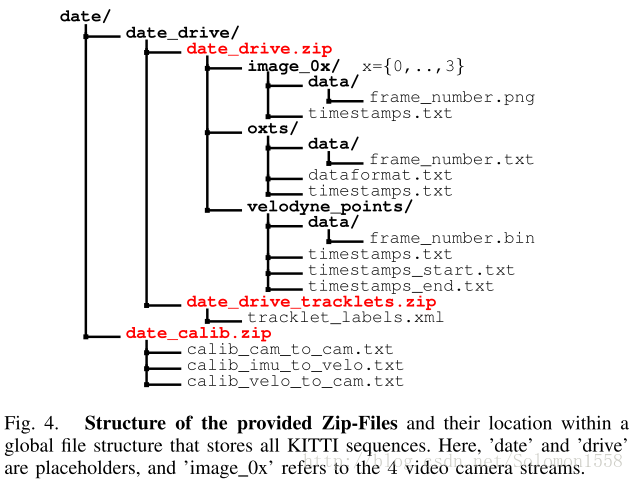
\includegraphics[width=0.75\textwidth]{SemanticSLAM/KITTI1.png}
\caption{早期的数据文件组织格式}
\label{KITTI1}
\end{figure}

而现在,对于从官网下载的各个分任务的数据集,其文件组织形式比较简单,以Object Detection为例,下面是Object detection Evaluation 2012 标准数据集中left color images 文件的目录结构,样本分别存储在testing和training数据集中。

\begin{verbatim}
data_object_image_2/
| -- testing/
|      | -- image_2/
| -- training/
|      | -- image_2/
|      | -- label_2/
\end{verbatim}

\subsubsection{Development Kit}

KITTI各个子数据集都提供开发工具 development kit,主要由cpp文件夹,matlab文件夹,mapping文件夹和readme.txt组成。

cpp文件夹主要包含评估模型的源代码evaluate\_object.cpp。Mapping文件夹中的文件记录训练集到原始数据集的映射,从而开发者能够同时使用激光雷达点云,gps数据,右边彩色摄像机数据以及灰度摄像机图像等多模态数据。Matlab文件夹中的工具包含读写标签,绘制2D/3D标注框,运行demo等工具。Readme.txt文件非常重要,详述介绍了某个子数据集的数据格式,benchmark介绍,结果评估方法等详细内容。

\subsection{Cityscape}

数据集官网:\href{https://www.cityscapes-dataset.com/}{Cityscapes Datasets}



\subsection{TUM}

数据集官网:\href{https://vision.in.tum.de/data/datasets}{TUM Datasets}

\section{实例分割-图像分割2018.06.11博客总结}

\subsection{Mask R-CNN狙击目标实例分割}

参考文献:\href{https://zhuanlan.zhihu.com/p/26047813}{Mask R-CNN 狙击目标实例分割-知乎}

\subsubsection{什么是实例分割}

举例子的方式:简单讲,一群人在图片里面,我希望把\textbf{每个人}都给我分割出来。分类只能做到识别这个图片是人;目标检测只能检测到这个图片里有人,把人的地方框出来,对每一个人这个个体不一样是没有判断的,统一认为是人;而图像分割主要是将人和背景分割出来,而实例分割就是要把每个人清晰的分割出来。

总的来说,Mask R-CNN是基于Faster R-CNN的基于上演进改良而来,FasterR-CNN并不是为了输入输出之间进行像素对齐的目标而设计的,为了弥补这个不足,我们提出了一个简洁非量化的层,名叫RoIAlign,RoIAlign可以保留大致的空间位置,除了这个改进之外,RoIAlign还有一个重大的影响:那就是它能够相对提高10\%到50\%的掩码精确度(Mask Accuracy),这种改进可以在更严格的定位度量指标下得到更好的度量结果。第二,我们发现分割掩码和类别预测很重要:为此,我们为每个类别分别预测了一个\textbf{二元}掩码。

\subsubsection{Mask RCNN介绍}
Mask R-CNN拥有简洁明了的思想:对于Faster R-CNN来说,对于每个目标对象,它有两个输出,一个是类标签(classlabel),一个是边界框的Offset(bounding-box offset),在此基础上,Mask R-CNN方法增加了第三个分支的输出:目标掩码。目标掩码与已有的class和box输出的不同在于它需要对目标的空间布局有一个更精细的提取。

\subsubsection{Mask RCNN的工作机理}

在Faster RCNN中,相比于Fast RCNN,多了一个Stage,那就是Region Proposal Network。所以在Faster RCNN中,整个算法由两个Stage构成,第一个Stage, 就是RPN, 这一步产生ROI,前面也提到了,在Fast RCNN中,输入既包括Image也包括一个ROI, 所以这里采用RPN来生成ROI。在第二Stage中,其实和Fast RCNN是一样的,都是借助ROI Pool来完成目标检测(目标分类+Bounding box offsets)。

那么在Mask RCNN中,在第二步骤中,与预测目标类别与Offset\textbf{平行的是}还会对每一个ROI输出一个Binary mask。所以Mask的branch, 会输出一个K*m*m大小的张量,其中K表示类别的个数。在实现过程中,

相应的,在训练的时候,也会采用一个多任务Loss Function:
\begin{displaymath}
L = L_{cls} + L_{box} + L_{mask}
\end{displaymath}

前两个Loss和Fast RCNN中是一样的,后面的mask的loss。有很多不懂的地方啊。

\subsubsection{Tensorflow + Keras实现实例分割}

参考文献:\href{https://mp.weixin.qq.com/s/Fo1yd6W1EdCQGEflP26tHA}{Tensorflow+Keras实现实例分割-微信公众号}

分割掩码是输入目标的空间布局编码,不像类别标签或边界框偏移量那样将特征经过全连接层“坍缩”到短的输出向量,而是自然地采用卷积实现“像素到像素”的变换,抽取掩码空间结构信息。使用 FCN 网络为每个 RoI 预测一个 mxm 掩码,这样允许它们保持 mxm 目标空间布局信息。

Mask RCNN 中使用 RoIAlign 替换了 RoIPool,RoIPool 没有考虑保留尽可能多的空间布局信息,难以实现输入图片/输出掩码像素一一对应。





























\chapter{MXNet}

参考文献:\href{https://mxnet.incubator.apache.org/architecture/index.html}{MXNet Architecture}

{\color{red}Time: 2018.05.18}

\section{Optimizing Memory Consumption in DL}
Over the last ten years, a constant trend in deep learning is towards deeper and larger networks. Despite rapid advances in hardware performance, cutting-edge deep learning models continue to push the limits of GPU RAM. So even today, it’s always desirable to find ways to train larger models while consuming less memory. Doing so enables us to train faster, using larger batch sizes, and consequently achieving a higher GPU utilization rate.

\subsection{Computation Graph}
A computation graph describes the (data flow) dependencies between the operations in the deep network. The operations performed in the graph can be either fine-grained or coarse-grained.

The concept of a computation graph is explicitly encoded in packages like Theano and CGT. In other libraries, computation graphs appear implicitly as network configuration files. The major difference in these libraries comes down to how they calculate gradients. There are mainly two ways: performing back-propagation on the same graph or explicitly representing a backwards path to calculate the required gradients.

\begin{figure}[!hbtp]
\centering
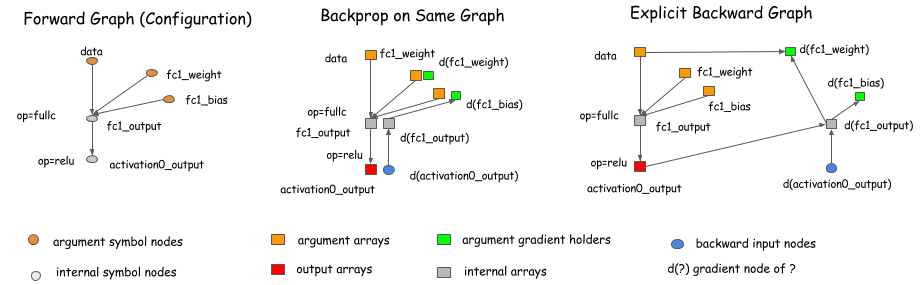
\includegraphics[width=0.85\textwidth]{MXNet/back_graph}
\caption{The implicitly \& explicitly back-propagation on Graph}
\end{figure}

Libraries like Caffe, CXXNet, and Torch take the former approach, performing back-prop on the original graph. Libraries like Theano and CGT take the latter approach, explicitly representing the backward path. In this discussion, we adopt the explicit backward path approach because it has several advantages for optimization.

We adopt the explicit backward path approach because it has several advantages for optimization.

Why is explicit backward path better? Two reasons:
\begin{itemize}
\item The explicit backward path clearly describes the dependency between computations.\\
Like the following case, where we want to get the gradient of \textbf{A} and \textbf{B}. As we can see clearly from the graph, the computation of the $d(C)$ gradient doesn’t depend on $F$. This means that we can free the memory of $F$ right after the forward computation is done. Similarly, the memory of $F$ can be recycled.
\begin{figure}[!hbtp]
\centering
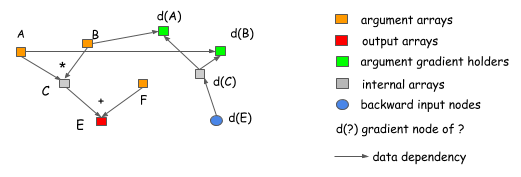
\includegraphics[width=0.85\textwidth]{MXNet/back_dep_prune}
\caption{Dependencies can be found quickly.}
\end{figure}

\item Another advantage of the explicit backward path is the ability to have a different backward path, instead of a mirror of forward one.\\
A common example is the split connectioncase, as shown in the following figure.
\begin{figure}[!hbtp]
\centering
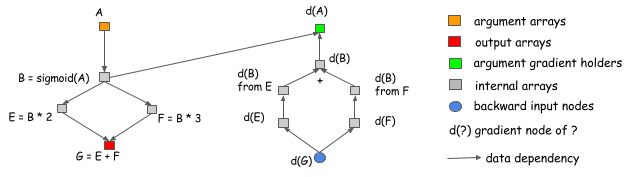
\includegraphics[width=0.85\textwidth]{MXNet/back_agg_grad}
\caption{Different backward path from forward path.}
\end{figure}
In this example, the output of \textbf{B} is referenced by two operations. If we want to do the gradient calculation in the same network, we need to introduce an explicit split layer. This means we need to do the split for the forward pass, too. In this figure, the forward pass doesn’t contain a split layer, but the graph will automatically insert a gradient aggregation node before passing the gradient back to \textbf{B}. This helps us to save the memory cost of allocating the output of the split layer, and the operation cost of replicating the data in the forward pass.
\end{itemize}

\subsection{What Can be Optimized?}
As you can see, the computation graph is a useful way to discuss memory allocation optimization techniques. Already, we’ve shown how you can save some memory by using the explicit backward graph. Now let’s explore further optimizations, and see how we might determine reasonable baselines for benchmarking.

Assume that we want to build a neural network with \textit{n} layers. Typically, when implementing a neural network, we need to allocate node space for both the output of each layer and the gradient values used during back-propagation. This means we need roughly $2n$ memory cells. We face the same requirement when using the explicit backward graph approach because the number of nodes in a backward pass is roughly the same as in a forward pass.

\subsubsection{In-place Operations}
One of the simplest techniques we can employ is \textit{In-place memory sharing} across operations. For neural networks, we can usually apply this technique for the operations corresponding to activation functions. 

''In-place'' means using same memory for input and output. But you should be careful about that the result is used by more than one operation! 

\subsubsection{Standard Memory Sharing}
In-place operations are not the only places where we can share memory. In the following example, because the value of B is no longer needed after we compute E, we can reuse B’s memory to hold the result of E.
\begin{figure}[!hbtp]
\centering
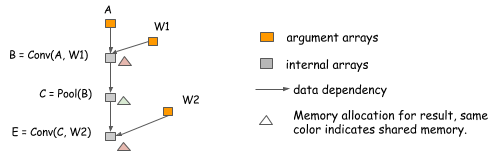
\includegraphics[width=0.85\textwidth]{MXNet/alloc_normal}
\caption{Standard Memory sharing between \textbf{B} \& the result of \textbf{E}.}
\end{figure}

Memory sharing doesn't necessarily require the same data shape. Note that in the preceding example, the shapes of \textbf{B} and \textbf{E} can differ. To handle such a situation, we can allocate a memory region of size equal to the maximum of that required by \textbf{B} and \textbf{E} and share it between them.

\subsection{Memory Allocation Algorithm}
Based on the '' In-Place Operatioins'', how can we allocate memory correctly?

The key problem is that we need to place resources so that they don’t conflict with each other. More specifically, each variable has a \textbf{life time} between the time it gets computed until the last time it is used. In the case of the multi-layer perceptron, the life time of \textit{fc1} ends after \textit{act1} get computed.
\index{Life Time}
See below figure:
\begin{figure}[!hbtp]
\centering
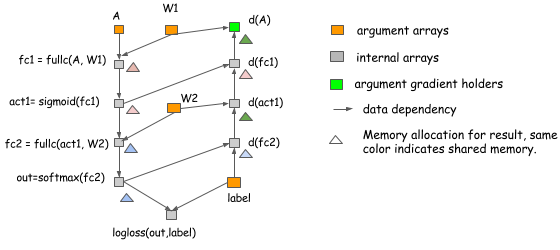
\includegraphics[width=0.85\textwidth]{MXNet/alloc_mlp}
\caption{Standard Memory sharing between \textbf{B} \& the result of \textbf{E}.}
\end{figure}

The principle is to allow memory sharing only between variables whose lifetimes don’t overlap. There are multiple ways to do this. You can construct the conflicting graph with each variable as a node and link the edge between variables with overlapping lifespans, and then run a graph-coloring algorithm. This likely has $O(n^2)$ complexity, where \textit{n} is the number of nodes in the graph. This might be too costly.

Let’s consider another simple heuristic. The idea is to simulate the procedure of traversing the graph, and keep a count of future operations that depends on the node.
\begin{figure}[!hbtp]
\centering
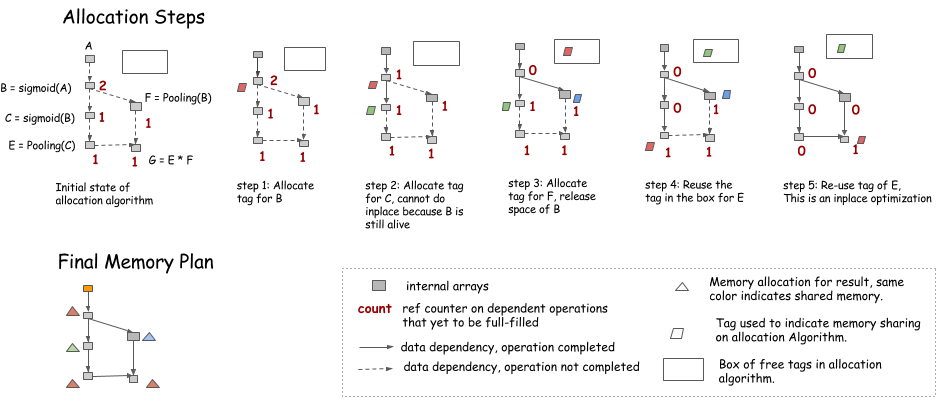
\includegraphics[width=0.95\textwidth]{MXNet/alloc_step}
\caption{Standard Memory sharing between \textbf{B} \& the result of \textbf{E}.}
\end{figure}
\begin{itemize}
\item An in-place optimization can be performed when only the current operation depends on the source (i.e. count == 1).
\item Memory can be recycled into the box on the upper right corner when the \textit{count} goes to 0.
\item When we need new memory, we can either get it from the box or allocate a new one. 
\end{itemize}

\textbf{Noet:} During the simulation, no memory is allocated. Instead, we keep a record of how much memory each node needs, and allocate the maximum of the shared parts in the final memory plan.

\subsection{Static vs. Dynamic Allocation}
The major difference is that static allocation is only done once, so we can afford to use more complicated algorithms. For example, we can search for memory sizes that are similar to the required memory block. The Allocation can also be made graph aware. We’ll talk about that in the next section. Dynamic allocation puts more pressure on fast memory allocation and garbage collection.

There is also one takeaway for users who want to rely on dynamic memory allocations: do not unnecessarily reference objects. For example, if we organize all of the nodes in a list and store then in a Net object, these nodes will never get dereferenced, and we gain no space. Unfortunately, this is a common way to organize code.

\subsection{Memory Allocation for Parallel Operations}
In the previous section, we discussed how we can simulate running the procedure for a computation graph to get a static allocation plan. However, optimizing for parallel computation presents other challenges because resource sharing and parallelization are on the two ends of a balance. Let’s look at the following two allocation plans for the same graph:
\begin{figure}[!hbtp]
\centering
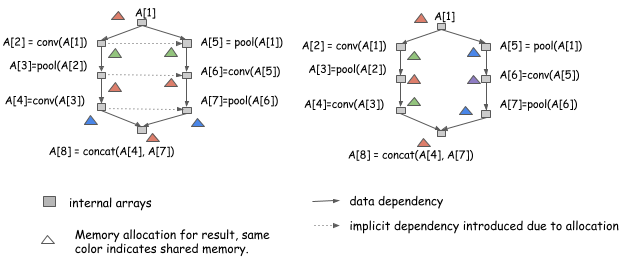
\includegraphics[width=0.95\textwidth]{MXNet/parallel_alloc}
\caption{Standard Memory sharing between \textbf{B} \& the result of \textbf{E}.}
\end{figure}

Both allocation plans are valid if we run the computation serially, {\bfseries from $A[1]$ to $A[8]$. } However, the allocation plan on the left introduces additional dependencies, which means we can't run computation of $A[2]$ and $A[5]$ in parallel. The plan on the right can. To parallelize computation, we need to take greater care. 

\subsubsection{Be Correct and Safe First}
Being correct is our first principle. This means to execute in a way that takes implicit dependency memory sharing into consideration. You can do this by adding the implicit dependency edge to the execution graph. Or, even simpler, if the execution engine is mutation aware, as described in \href{https://mxnet.incubator.apache.org/architecture/note_engine.html}{our discussion of dependency engine design}, push the operation in sequence and write to the same variable tag that represents the same memory region.

Always produce a safe memory allocation plan. This means never allocate the same memory to nodes that can be parallelized. This might not be ideal when memory reduction is more desirable, and we don’t gain too much when we can get benefit from multiple computing streams simultaneously executing on the same GPU.

\subsubsection{Try to Allow More Parallelization}
Now we can safely perform some optimizations. The general idea is to try and encourage memory sharing between nodes that can’t be parallelized. You can do this by creating an ancestor relationship graph and querying it during allocation, which costs approximately $O(n^2)$ in time to construct. We can also use a heuristic here, 
for example, color the path in the graph. As shown in the following figure, when you try to find the longest paths in the graph, color them the same color and continue.
\begin{figure}[!hbtp]
\centering
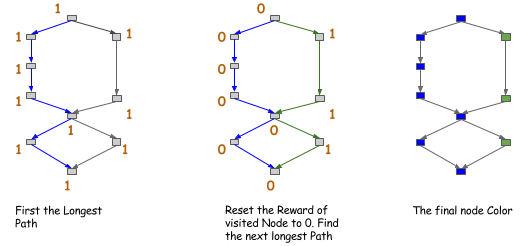
\includegraphics[width=0.95\textwidth]{MXNet/graph_color}
\caption{Color the longest paths in the Graph.}
\end{figure}

After you get the color of the node, you allow sharing (or encourage sharing) only between nodes of the same color. This is a stricter version of the ancestor relationship, but is costs only $O(n)$ of time if you search for only the first $k$ path.

\subsection{How Much Can we Save ?}
On coarse-grained operation graphs that are already optimized for big operations, you can reduce memory consumption roughly by half. You can reduce memory usage even more if you are optimizing a fine-grained computation network used by symbolic libraries, such as Theano.

\subsection{References}
More details can be found in: \href{https://mxnet.incubator.apache.org/architecture/note_memory.html#how-much-can-you-save}{Opimizing the Memory Consumption in DL(MXNet)}.


\section{Deep Learning Programming Style}

Two of the most important high-level design decisions

\begin{itemize}
\item Whether to embrace the symbolic or imperative paradigm for mathematical computation

\item Whether to build networks with bigger or more atomic operations
\end{itemize}

\subsection{Symbolic vs. Imperative Program}

即:符号式编程 vs. 命令式编程

Symbolic programs are a bit different. With symbolic-style programs, we first define a (potentially complex) function abstractly. When defining the function, no actual numerical computation takes place. We define the abstract function in terms of \textbf{placeholder values}(占位符). Then we can compile the function, and evaluate it given real inputs. 

This operation generates a computation graph (also called a symbolic graph) that represents the computation.

Most symbolic-style programs contain, either explicitly or implicitly, a compile step. 

真正的计算只发生在传入数值之时,在这之前,都没有任何计算发生。

The defining characteristic of symbolic programs is their clear separation between building the computation graph and executing it.For neural networks, we typically define the entire model as a single compute graph.

\subsection{Imperative Programs Tend to be More Flexible}

使用命令式编程,那么任何Python语法都可以使用(Nearly anything),但使用符号式编程时,一些Python特性可能无法使用,如迭代。

当使用Python的符号式编程时,实际实在一个Domain-Specific-Language(DSL)定义的空间中进行编程。

Intuitively, you might say that imperative programs are more native than symbolic programs. It’s easier to use native language features. 

\subsection{Symbolic Programs Tend to be More Efficient}

命令式编程与原生Python的相差不大,所以灵活性很高。但符号式编程更有利于速度、存储优化。

Symbolic programs are more restricted. When we call \textit{Compile} on d, we tell the system that only the value of d is needed. The intermediate values of the computation, is then invisible to us.

\begin{itemize}
\item We benefit because the symbolic programs can then safely reuse the memory for in-place computation. 

\item Symbolic programs can also perform another kind of optimization, called operation folding(图\ref{Symbolic1}). In fact, this is one way we hand-craft operations in optimized libraries, such as CXXNet and Caffe. Operation folding improves computation efficiency.

\begin{figure}
\centering
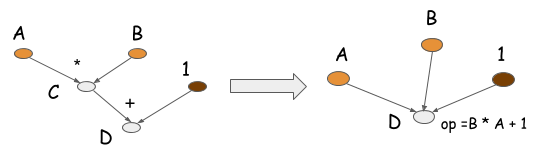
\includegraphics[width=0.75\textwidth]{MXNet/Symbolic1.png}
\caption{Operation Folding示意图。}
\label{Symbolic1}
\end{figure}

Note, you can’t perform operation folding in imperative programs, because the intermediate values might be referenced in the future. Operation folding is possible in symbolic programs because you get the entire computation graph, and a clear specification of which values will be needed and which are not.
\end{itemize}

\subsection{Case Study: Backprop and AutoDiff}
\lstset{language=Python}
\begin{lstlisting}[title=toy model,frame=shadowbox]
import numpy as np
    a = np.ones(10)
    b = np.ones(10) * 2
    c = b * a
    d = c + 1
    ...
\end{lstlisting}


\subsubsection{基于命令式编程的自动求导}
循环调用求导函数,直至最开始的输入变量。

利用grad闭包(Closure)来隐含的保存后向计算图。

但一个坏处是,必须保存所有中间变脸的Grad闭包。

\subsubsection{基于符号式编程的自动求导}

可以实现的优化力度更大。

\subsubsection{Analysis}

可以实现的优化的程度,依赖于可以允许的操作(Restrictions on what you can do)。使用符号式编程时,必须明确提供这些约束,所以可进行优化也就更多。

对于命令式编程,可以通过其它的一些方式添加明确的约束。比如一种方法是Context Variable。如:
\begin{verbatim}
with context.NoGradient()
    ...
\end{verbatim}
可以关闭梯度的计算。但这样也不能利用In-Place Calculation来对存储空间进行复用。

其实是一种trade-off between restriction and flexibility.

\subsection{Model Checkpoint}

保存和加载模型。保存模型的时候,需要保存两类变量:网络的结构配置、网络的权重系数。

符号式编程有利于配置的检查。而对于命令式编程,需要保存所有的代码,或者利用符号式指令进行能够顶层封装。

\begin{itemize}
\item Parameter Updates

大部分符号是编程,都是基于数据流图(Data Flow Graphs, DFG)实现的。DFG描述的是计算。但这种方式下,参数的更新不是很方便。一些做法是将更新过程转化为基于命令式的方式实现,而梯度的计算是基于计算图的方式计算。

\item There is No Strict Boundary

这两种风格的框架其实没有很明显的区分。如在命令式编程时,可以借助Just-in-Time(JIT) Compiler来实现一些符号式编程里面的全局优化等好处。
 
\end{itemize}


\subsection{Big vs. Small Operations}

\begin{itemize}
\item Big Operations

主要是一些经典的神经网络层在用,如Fully Connected and Batch Normalize.

\item Small Operations

一些数学上的计算,如矩阵乘、Element-wise Addition.

\end{itemize}

CXXNet, Caffe支持Layer一级的计算,而Theano, Minerva支持更精细的计算。

\begin{itemize}
\item Smaller Operations Can Be More Flexible (小运算更灵活)

可实现的东西多,且建立新的Layer比较简单,直接添加部件就行。

\item Big Operations Are More Efficient (大运算更高效)

可能引起计算、存储上的开支。

\item Compilation and Optimization

对于小运算的优化,计算图支持一下两种优化:
\begin{itemize}
\item Memory Allocation Optimization

重用中间结果的存储空间。也可用于大运算。

\item Operator Fusion

Fuse several small operations into big one.

\end{itemize}

这些优化对小操作十分重要。小操作对编译器也增加了负担。

\item Expression Template and Statically Typed Language

借助Expression Template来产生具体的Kernels.\href{https://github.com/dmlc/mshadow/blob/master/guide/exp-template/README.md}{Template Expression}, 其实底层是基于C++ Template实现的。

\end{itemize}


\subsection{Mix The Approaches}

Amdahl's Law:
\begin{quote}
 If you are optimizing a non-performance-critical part of your problem, you won’t get much of a performance gain
\end{quote}

实际考虑编程Style时,需要综合考虑:性能、灵活性、工程复杂度等。实践表明,混合使用多个Style可以得到更好的性能。

\begin{itemize}
\item Symbolic and Imperative Programs

有两种方式可以实现这种混用:
\begin{itemize}
\item Use imperative programs within symbolic programs as callbacks
\item Use symbolic programs as part of imperative programs
\end{itemize}
如在参数更新中的讨论。如果代码中,混合了Symbolic和Imperative,那么结果是Imperative.但更好的选择是,用支持GPU计算、参数更新的符号式编程框架来开发。

\item Small and Big Operations
\item Choose Your Own Approach
\end{itemize}

\section{Dependency Engine for Deep Learning}

\subsection{Problems in Dependency Scheduling}

\begin{itemize}
\item Data Flow Dependency

Data flow dependency describes how the outcome of one computation can be used in other computations. 

\item Memory Recycling

\item Random Number Generation

A pseudo-random number generator (PRNG) is not thread-safe because it might cause some internal state to mutate when generating a new number. Even if the PRNG is thread-safe, it is preferable to serialize number generation, so we can get reproducible random numbers.

\end{itemize}

\subsubsection{Design a Generic Dependency Engine}

目标是建立一个轻量级、普用的依赖引擎。目标如下:
\begin{itemize}
\item 识别有效的操作
\item 可以调度GPU、CPU存储的依赖,以及处理随机发生器的依赖
\item 引擎不应分配资源,而仅处理依赖
\end{itemize}

步骤如下:

\begin{enumerate}
\item At the beginning, the user can allocate the variable tag, and attach it to each of the objects that we want to schedule.

\begin{figure}[!hbtp]
\centering
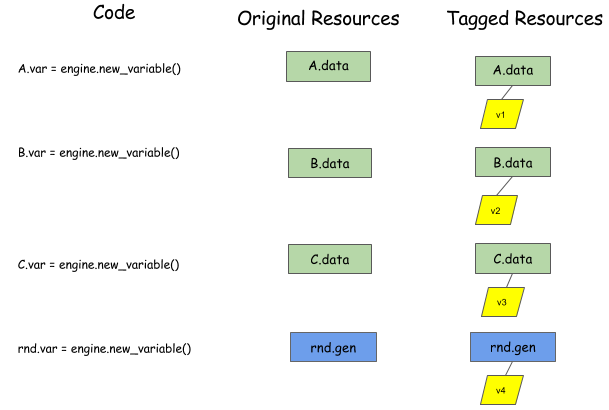
\includegraphics[width=0.75\textwidth]{MXNet/Tag1.png}
\caption{第一步,给变量分配tag}
\label{Tag1}
\end{figure}

\item 然后调用\textit{push}来告知引擎需要运行的函数、参数等,需要区分读取、写入的参数,分别输入。引擎通过识别上一步的tag来识别变量,这样的好处是不涉及tag具体指向什么,所以引擎可以处理包括变量、函数之类的Everything。

\begin{figure}[!hbtp]
\centering
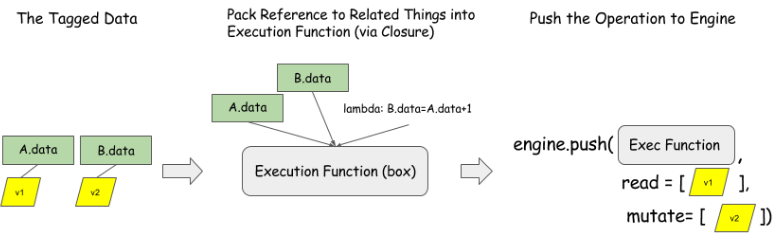
\includegraphics[width=0.75\textwidth]{MXNet/Tag2.png}
\caption{把相应的Function Closure push进依赖分析引擎}
\label{Tag2}
\end{figure}
\end{enumerate}

\subsection{Implementing the Generic Dependency Engine}

基本思想
\begin{itemize}
\item Use a queue to track all of the pending dependencies on each variable tag
\item Use a counter on each operation to track how many dependencies are yet to be fulfilled
\item When operations are completed, update the state of the queue and dependency counters to schedule new operations
\end{itemize}

一个例子如图所示:
\begin{figure}[!hbtp]
\centering
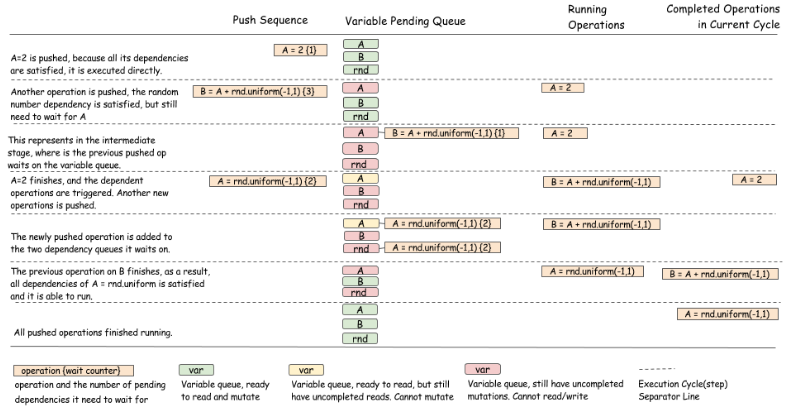
\includegraphics[width=0.95\textwidth]{MXNet/Tag3.png}
\caption{一个具体的例子}
\label{Tag3.png}
\end{figure}

\subsection{Discussion}

\begin{itemize}
\item Dynamic vs. Static
\item Mutation vs. Immutable
\end{itemize}

\section{Designing Efficient Data Loaders for DL}

几点重要的考虑:
\begin{itemize}
\item Small File Size
\item Parallel (Distributed) packing of data
\item Fast data loading and online augmentation
\item Quick reads from arbitrary parts of the dataset in the distributed setting
\end{itemize}

\subsection{Design Insight}

为了设计好的IO系统,需要解决两类任务:Data Preparation, Data Loading.

\subsubsection{Data Preparation}

Data preparation describes the process of packing data into a desired format for later processing. 

\begin{itemize}
\item Pack the dataset into small numbers of files
\item Do the packing once
\item Process the packing in parallel to save time
\item Be able to access arbitrary parts of the data easily
\end{itemize}

\subsubsection{Data Loading}

The next step to consider is how to load the packed data into RAM. 

\begin{itemize}
\item Read Continuously
\item Reduce the bytes to be loaded,可以借助于数据压缩等
\item Load and train in different threads
\item Save RAM
\end{itemize}

\subsection{Data Format}

需要选择既高效又方便的数据结构。为了实现这个目标,把二进制数据包装成可以分离的结构。具体,MXNet采用DMLC-Core里面的recordIO类型。

\begin{figure}[!hbtp]
\centering
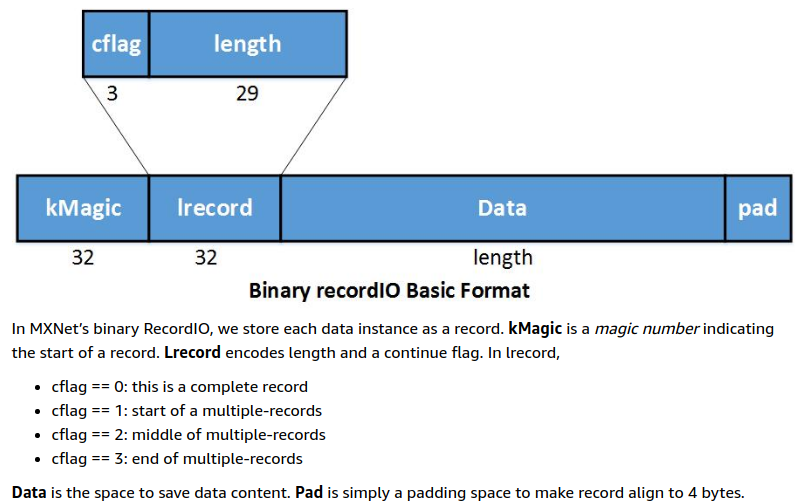
\includegraphics[width=0.95\textwidth]{MXNet/recordIO1.png}
\caption{Binary recordIO数据结构}
\label{recordIO1}
\end{figure}

通过连续读,来避免随机读引入的延时。

这种数据结构的一个好处是,每一个record的长度可以改变。从而支持更好的数据压缩。

\begin{figure}[!hbtp]
\centering
\includegraphics[width=0.95\textwidth]{MXNet/recordIO2.png}
\caption{Binary recordIO的一个例子}
\label{recordIO2}
\end{figure}
其中,\textit{resize}把输入图像变为256 * 256大小。


\subsubsection{Access Arbitrary Parts of Data}

The packed data can be logically sliced into an arbitrary number of partitions, no matter how many physical packed data files there are.

在recordIO中借助Magic Number来实现上述目的,具体是使用dmlc-core中的\textit{InputSplit}函数来实现。这个函数极大的帮助了并行实现,因为每一个节点只处理一个\textit{Part}.

\subsection{Data Loading and Preprocessing}

\subsubsection{Loading and Preprocessing on the Fly}

In service of efficiency, we also address multi-threading techniques. 

\begin{figure}[!hbtp]
\centering
\includegraphics[width=0.95\textwidth]{MXNet/loadingData1.png}
\caption{并行预处理例子}
\label{loadingData1}
\end{figure}

在加载了大量图像数据后,利用多线程工具(OpenMP)进行并行处理。

\subsubsection{Hide IO Cost Using Threadediter}

一种降低IO影响的办法是:数据预取。具体使用dmlc-core提供的\textit{threadediter}来处理IO. The key of threadediter is to start a stand-alone thread that acts as a data provider, while the main thread acts as a data consumer as illustrated below.

The threadediter maintains a buffer of a certain size and automatically fills the buffer when it’s not full. And after the consumer finishes consuming part of the data in the buffer, threadediter will reuse the space to save the next part of data. 

\begin{figure}[!hbtp]
\centering
\includegraphics[width=0.95\textwidth]{MXNet/dataLoading2.png}
\caption{数据预取的示意图,借助Buffer来实现}
\label{loadingData2}
\end{figure}


\subsection{MXNet IO Python Interface}

We make the IO object as an iterator in numpy. By achieving that, the user can easily access the data using a for-loop or calling next() function. Defining a data iterator is very similar to defining a symbolic operator in MXNet.

为了创建一个数据迭代器,需要提供五种类型的参数:

\begin{itemize}
\item Dataset Param: 如路径、输入的尺寸等
\item Batch Param: Batch Size
\item Augmentation Param: 确定数据增广的类型,如翻转等
\item Backedn Param:  控制后台线程,来隐藏数据读取延时
\item Auxiliary Param: 帮助Debug的信息等。
\end{itemize}

通常必须确定\textbf{Dataset Param}和\textbf{Batch Param}。MX Data IO也支持模块化,如以下两种:
\begin{itemize}
\item 自己的高效数据预取。allows the user to write a data loader that reads their customized binary format that automatically gets multi-threaded prefetcher support.

\item 数据转换。image random cropping, mirroring, etc. Allows the users to use those tools, or plug in their own customized transformers

\end{itemize}


\section{Except Handling in MXNet}

MXNet在两类情况下可以抛出异常:
\begin{itemize}
\item MXNet main thread. For \textit{e.g.} Infershape and InferType。 在主线程中处理
\item Spawned threads (生成线程?)
\begin{itemize}
\item By dependency engine for operator execution in parallel。会被rethrown到主线程,进行处理
\item By the iterators, during the data loading, text parsing phase \textit{etc.}
\end{itemize}
\end{itemize}

\subsubsection{Exception Handling for Iterators}

CVIter 使用 PrefetcherIter来加载和解析数据。PrefetcherIter会生成一个Producer线程并后台运行,在主线程(Consumer)中使用这些数据。在Producer线程中可能抛出异常,该异常被发送到主线程。


可能引起线程之间的竞争(Race).To avoid this situation, you should try and iterate through your full dataset if you think it can throw exceptions which need to be handled.

\subsubsection{Except Handling for Operators}

For the operator case, the dependency engine spawns a number of threads if it is running in the \textbf{ThreadedEnginePool} or \textbf{ThreadedEnginePerDevice} mode. The final operator is executed in one of the spawned threads.

If an operator throws an exception during execution, this exception is propagated down the dependency chain. Once there is a synchronizing call i.e. \textbf{WaitToRead} for a variable in the dependency chain, the propagated exception is rethrown.


\textbf{注意}:Please avoid waitalls in your code unless you are confident about your code not throwing exception in any scenario. 因为\textbf{mx.nd.waitall}不支持rethrowing异常。

\section{MXNet-Gluon创建模型}

参考文献:\href{zh.gluon.ai}{Gluon}

\subsection{模型构造}

继承\verb|gluon.nn.Block|来实现,必须重载\verb|forward|函数。在\verb|__init__|函数里面定义模型所需的变量等。

\textbf{需要值得注意的地方是},在基于自定义的模型构建大的模型时,需要调用的是\verb|__init__|函数的参数;而一旦模型定义好了,开始向里面传入数据时,数据的格式需要根据\verb|forward|函数来确定!

\subsubsection{两种稍微不同的实现}
方式一,是直接利用Gluon预定义的层构建类型变量。
\lstset{language=Python, caption={自定义模型,方式一}, label=MXNetModel0}
\begin{lstlisting}
from mxnet import nd
from mxnet.gluon import nn

class MLP(nn.Block):
    # 声明带有模型参数的层,这里我们声明了两个全链接层。
    def __init__(self, **kwargs):
        # 调用 MLP 父类 Block 的构造函数来进行必要的初始化。这样在构造实例时还可以指定
        # 其他函数参数,例如下下一节将介绍的模型参数 params。
        super(MLP, self).__init__(**kwargs)
        # 隐藏层。
        self.hidden = nn.Dense(256, activation='relu')
        # 输出层。
        self.output = nn.Dense(10)
    # 定义模型的前向计算,即如何根据输出计算输出。
    def forward(self, x):
        return self.output(self.hidden(x))
\end{lstlisting}

方式二,即先定义一个Sequential的类型变量Net,然后在向里面增加\verb|gluon.nn.Layer|等具体的层,或者自己定义的层。
\lstset{language=Python, caption={自定义模型,方式二}, label=MXNetModel1}
\begin{lstlisting}
class NestMLP(nn.Block):
    def __init__(self, **kwargs):
        super(NestMLP, self).__init__(**kwargs)
        self.net = nn.Sequential()
        self.net.add(nn.Dense(64, activation='relu'),
                     nn.Dense(32, activation='relu'))
        self.dense = nn.Dense(16, activation='relu')

    def forward(self, x):
        return self.dense(self.net(x))  #调用要加self

net = nn.Sequential()
net.add(NestMLP(), nn.Dense(20), FancyMLP())

net.initialize()
net(x)
\end{lstlisting}

由于FancyMLP和Sequential都是Block的子类,我们可以嵌套调用他们。

实际使用中,貌似还存在第三种构建方式,直接以函数的形式使用, 如VGG:
\lstset{language=Python, caption={自定义模型VGG11,方式三}, label=MXNetLayer2}
\begin{lstlisting}
import sys
sys.path.append('..')
import gluonbook as gb
from mxnet import nd, init, gluon
from mxnet.gluon import nn

def vgg_block(num_convs, num_channels):
    blk = nn.Sequential()
    for _ in range(num_convs):
        blk.add(nn.Conv2D(
            num_channels, kernel_size=3, padding=1, activation='relu'))
    blk.add(nn.MaxPool2D(pool_size=2, strides=2))
    return blk
conv_arch = ((1,64), (1,128), (2,256), (2,512), (2,512))

def vgg(conv_arch):
    net = nn.Sequential()
    # 卷积层部分
    for (num_convs, num_channels) in conv_arch:
        net.add(vgg_block(num_convs, num_channels))
    # 全连接层部分
    net.add(nn.Dense(4096, activation="relu"), nn.Dropout(.5),
            nn.Dense(4096, activation="relu"), nn.Dropout(.5),
            nn.Dense(10))
    return net

net = vgg(conv_arch)
\end{lstlisting}

\subsection{自定义层}

也需要继承\verb|gluon.nn.Block|以及重载\verb|forward|函数。

\lstset{language=Python, caption={自定义层,方式一}, label=MXNetLayer0}
\begin{lstlisting}
class CenteredLayer(nn.Block):
    def __init__(self, **kwargs):
        super(CenteredLayer, self).__init__(**kwargs)

    def forward(self, x):
        return x - x.mean()
\end{lstlisting}

\subsubsection{带参数的自定义层}

我们还可以自定义含模型参数的自定义层。这样,自定义层里的模型参数就可以通过训练学出来了。我们在“模型参数”一节里介绍了Parameter类。其实,在自定义层的时候我们还可以使用Block自带的ParameterDict类型的成员变量params。顾名思义,这是一个由字符串类型的参数名字映射到Parameter类型的模型参数的字典。我们可以通过get函数从ParameterDict创建Parameter,注意是创建,也就是加入!

\lstset{language=Python, caption={带参数的自定义层,方式一}, label=MXNetLayer1}
\begin{lstlisting}
class MyDense(nn.Block):
    def __init__(self, units, in_units, **kwargs):
        super(MyDense, self).__init__(**kwargs)
        self.weight = self.params.get('weight', shape=(in_units, units))
        self.bias = self.params.get('bias', shape=(units,))

    def forward(self, x):
        linear = nd.dot(x, self.weight.data()) + self.bias.data()
        return nd.relu(linear)
\end{lstlisting}

\subsection{实际例子}

\subsubsection{ResNet}

使用的是自定义层方式一中的方式构建残差块。然后定义更高一级的结构(自定义模型方式二中的方法),最后再在更高一级进行构架整个模型。层次结构如下:

\lstset{language=Python, caption={ResNet using Gluon}}
\begin{lstlisting}
import sys
sys.path.append('..')
import gluonbook as gb
from mxnet import nd, gluon, init
from mxnet.gluon import nn

# 构建底层
class Residual(nn.Block):
    def __init__(self, num_channels, use_1x1conv=False, strides=1, **kwargs):
        super(Residual, self).__init__(**kwargs)
        self.conv1 = nn.Conv2D(num_channels, kernel_size=3, padding=1,
                               strides=strides)
        self.conv2 = nn.Conv2D(num_channels, kernel_size=3, padding=1)
        if use_1x1conv:
            self.conv3 = nn.Conv2D(num_channels, kernel_size=1,
                                   strides=strides)
        else:
            self.conv3 = None
        self.bn1 = nn.BatchNorm()
        self.bn2 = nn.BatchNorm()

    def forward(self, X):
        Y = nd.relu(self.bn1(self.conv1(X)))
        Y = self.bn2(self.conv2(Y))
        if self.conv3:
            X = self.conv3(X)
        return nd.relu(Y + X)

# 构建高一层        
def resnet_block(num_channels, num_residuals, first_block=False):
    blk = nn.Sequential()
    for i in range(num_residuals):
        if i == 0 and not first_block:
            blk.add(Residual(num_channels, use_1x1conv=True, strides=2))
        else:
            blk.add(Residual(num_channels))
    return blk
    
# 构建整个模型
net.add(resnet_block(64, 2, first_block=True),
        resnet_block(128, 2),
        resnet_block(256, 2),
        resnet_block(512, 2))        
\end{lstlisting}

需要注意的是,即使在\verb|class|里面也可以调用底层的自定义模块,如在\verb|resnet_block|中调用\verb|Residual|,具体调用方式是调用底层类的构造函数,即\verb|__init__|函数,参数要跟这个函数的参数一致。

\subsubsection{DenseNet}

发现与上面的ResNet类似,所以这里省略。

\section{MXNet中的Deconvolution}

具体实现是, \verb|Conv2DTranspose|等。

由于\verb|Conv2DTranspose|这个函数回引起棋盘状 Artifacts,所以在MXNet里面,还有一个上采样卷积的函数:\verb|mxnet.ndarray.UpSampling()|, \textbf{但是}, 听说目前还不好用啊。

参考\href{https://discuss.gluon.ai/t/topic/3041/14}{FCN讨论区-chen0510566}回答,\verb|gluon.nn.Conv2DTranspose|的文档,\verb|Conv2DTranspose|输出的size是这样计算的:
\begin{displaymath}
\begin{gathered}
Out\_height = (height - 1) * strides[0] - 2 * padding[0] + kernel\_size[0] + output\_padding[0] \\
Out\_width = (width - 1) * strides[1] - 2 * padding[1] + kernel\_size[1] + output\_padding[1]
\end{gathered}
\end{displaymath}

$\uparrow$正确性有待验证。

\section{MXNet读取训练数据}

重要,我发现,对于我这样的新手来说,如何处理数据也是个问题,尤其现在,我感觉一头雾水。

参考文章:

[1] \href{https://www.jianshu.com/p/38d55c9dbdb8}{MXNet常见加载数据的方式-简书}

[2] \href{https://mxnet.incubator.apache.org/api/python/io/io.html}{MXNet API}


有必要对MXNet的数据结构进行说明一下!尤其对于axes的概念。在MXNet中,我认为axes可以取四个值,分别对应以下概念:
\begin{itemize}
\item axes = 0, Batches, 比如batchsize=8, 那么axes就对应这8个样本
\item axes = 1, Channels, 比如输入彩色图像,那么axes对应的就是RGB三个通道
\item axes = 2, Width or Height, 还不太确定,与axes=3共同确定每一个Channel的尺寸
\end{itemize}

接下来就是本小节的重点内容,也就是如果处理训练数据,这是开始的一步,但我感觉也是容易被各种教程忽视的一步,如果这步不清楚,那么会影响整个后面的学习与实践过程。

{\bfseries 正如参考文献中所总结的那样,一共可以分为三类。分别如下!}

\begin{itemize}
\item 基于mxnet.io读取数据
\item 使用mxnet.iamge读取数据
\item \textbf{使用gluon接口读取数据}, 这个部分是重点
\end{itemize}

此外,作者还提到了几种支持的数据结构,貌似就这几种么?
\begin{itemize}
\item .rec文件
\item raw image
\item .lst文件,使用mx.image.ImageIter接口读取,这个接口可以读.rec的文件
\end{itemize}

大概流程:传data iter对象给base\_module,把数据对象变为iterator。
下面分别对三种数据读取方式进行示例。

\subsection{使用mx.io读取数据}

\subsubsection{从内存中读取}

调用\verb|mx.io.NDArrayIter|接口,以MXNet官方的train\_mnist.py为例。

\lstset{language=Python, caption={train\_mnist.py例子}}
\begin{lstlisting}
def read_data(label, image):
   """
   download and read data into numpy
   """
   base_url = 'http://yann.lecun.com/exdb/mnist/'
   with gzip.open(download_file(base_url+label, os.path.join('data',label))) as flbl:
       magic, num = struct.unpack(">II", flbl.read(8))
       label = np.fromstring(flbl.read(), dtype=np.int8)
   with gzip.open(download_file(base_url+image, os.path.join('data',image)), 'rb') as fimg:
       magic, num, rows, cols = struct.unpack(">IIII", fimg.read(16))
       image = np.fromstring(fimg.read(), dtype=np.uint8).reshape(len(label), rows, cols)
   return (label, image)


def to4d(img):
   """
   reshape to 4D arrays
   """
   return img.reshape(img.shape[0], 1, 28, 28).astype(np.float32)/255

def get_mnist_iter(args, kv):
   """
   create data iterator with NDArrayIter
   """
   (train_lbl, train_img) = read_data(
           'train-labels-idx1-ubyte.gz', 'train-images-idx3-ubyte.gz')
   (val_lbl, val_img) = read_data(
           't10k-labels-idx1-ubyte.gz', 't10k-images-idx3-ubyte.gz')
   train = mx.io.NDArrayIter(
       to4d(train_img), train_lbl, args.batch_size, shuffle=True)
   val = mx.io.NDArrayIter(
       to4d(val_img), val_lbl, args.batch_size)
   return (train, val)
#参考train_mnist.py
\end{lstlisting}

详解如下:
\begin{itemize}
\item 顶层函数为\verb|get_mnist_iter|函数

该函数的参数是:包含batch size的类arg。kv参数,但貌似没用到。

函数\verb|get_mnist_iter|调用\verb|read_data|函数,返回图像数据及其对应的label。该函数的

将\verb|read_data|函数的返回值传入\verb|mx.io.NDArrayIter|函数,该函数返回名称为\verb|train|和\verb|val|的data iterator. 分别作用与训练图像与训练标签。\verb|NDAarrayIter|函数的使用参数解释在下文单独总结。

返回data iterator的训练图像与训练标签。

\item 被调用函数\verb|read_data|

该函数在这里主要负责下载数据文件(download\_file())、解压缩(struct.unpack)等。各个函数的输入输出可参考源代码。

\item 被调用函数\verb|to4d|

负责把输入图片rehape成四维数据结构,维度分解见上文中的axes的解释。

\end{itemize}

所以总结一下的话,就是这样的,首先下载文件并解压缩,然后读取数据,送入\verb|mx.io.NDArrayIter|产生data iterator.

\subsubsection{从.csv文件中读取数据}

\lstset{language=Python, caption={Read .csv 数据}}
\begin{lstlisting}
#lets save `data` into a csv file first and try reading it back
np.savetxt('data.csv', data, delimiter=',')
data_iter = mx.io.CSVIter(data_csv='data.csv', data_shape=(3,), batch_size=30)
for batch in data_iter:
   print([batch.data, batch.pad])
\end{lstlisting}

详解:
\begin{itemize}
\item 调用\verb|mx.io.CSVIter|读取.csv格式文件,同时输入数据shape以及batch size。返回的就是一个 data iterator。
\end{itemize}

\subsubsection{使用mx.io.ImageRecordIter接口,需要定制KVStore}

这一部分还没看明白,可以看一下原文。

\subsection{常用的系统提供的接口函数}
分析以上实现方式,主要涉及以下几个系统接口函数。
\begin{itemize}
\item \verb|mx.io.NDArrayIter|

原型:class mxnet.io.NDArrayIter(data, label=None, batch\_size=1, shuffle=False, last\_batch\_handle='pad', data\_name='data', label\_name='softmax\_label')

其中,data, label为array 或list of array or dict of string to array。

last\_batch\_handle为最后一个batch的处理,即训练数据的数目不能被batch size整除时的处理方式,可以选取'pad', 'discard' or 'roll\_over'等。

更多细节见文档吧。

Returns an iterator for mx.nd.NDArray, numpy.ndarray, h5py.Dataset mx.nd.sparse.CSRNDArray or scipy.sparse.csr\_matrix.


\item \verb|mx.io.CSVIter|

return the CSV file iterator,详情见文档吧。

\item \verb|struct.unpack|

原型:\verb|struct.unpack(fmt, buffer)|

Unpack from the buffer buffer (presumably packed by pack(fmt, ...)) according to the format string fmt. The result is a tuple even if it contains exactly one item. The buffer’s size in bytes must match the size required by the format, as reflected by calcsize().关于fmt的具体格式,参考\href{https://docs.python.org/3/library/struct.html}{struct library python}

\item \verb|gzip.read()|

原型:\verb|read(size=-1)|

Read and return up to size bytes. If the argument is omitted, None, or negative, data is read and returned until EOF is reached. An empty bytes object is returned if the stream is already at EOF.

If the argument is positive, and the underlying raw stream is not interactive, multiple raw reads may be issued to satisfy the byte count (unless EOF is reached first). But for interactive raw streams, at most one raw read will be issued, and a short result does not imply that EOF is imminent.

所以参数是要读取的byte的数目。

\end{itemize}

\subsection{使用mx.image读取数据}

从imagelist中读取可迭代的数据。

\lstset{language=Python, caption={mx.image使用示例}}
\begin{lstlisting}
data_iter = mx.image.ImageIter(batch_size=4, data_shape=(3, 224, 224), label_width=1,
data_iter.reset()
for data in data_iter:
d = data.data[0]
print(d.shape)
# we can apply lots of augmentations as well
data_iter = mx.image.ImageIter(4, (3, 224, 224), path_imglist='data/custom.lst',
data = data_iter.next()
# specify augmenters manually is also supported
data_iter = mx.image.ImageIter(32, (3, 224, 224), path_rec='data/caltech.rec',
\end{lstlisting}

详解:
\begin{itemize}
\item 调用\verb|mx.image.ImageIter|实现
\end{itemize}

\subsection{使用Gluon接口读取数据}

由于用的比较多,所以这部分是重点,起码目前来看是重点。

使用Gluon接口时,我觉着主要分为两步:产生Dataset,基于Dataset产生 Mini-batch iterator!

下面分别对这两个步骤进行简单说明,后续有时间在详细说一下吧。通过本小节的简单解释,然后再看这个文档,应该就不那么难了吧,就知道各个部分是什么意思了,怎么组织在一起的了。

具体的参考文档:\href{https://mxnet.incubator.apache.org/api/python/gluon/data.html}{Gluon API 文档}

\subsubsection{产生Dataset}

Dataset的生成主要分为几种方式,这里主要讨论三种形式:
\begin{itemize}
\item Gluon自带的数据库,包括:MNIST, FashionMNIST, CIFAR10, CIFAR100等。

产生Dataset的方式为:

\begin{verbatim}
data_set = gluon.data.vision.Dataset
\end{verbatim}

其中, Dataset需要替换成提到的提供的自带数据库。

\item 来自目录生成Dataset, 调用:\verb|ImageFolderDataset|, 目录中保存的raw image。

产生Dataset的方式:

\begin{verbatim}
data_set = gluon.data.vision.ImageFolderDataset(root, flag=1, tranform=None)
\end{verbatim}

A dataset for loading image files stored in a folder structure like:看文档,ImageFolderDataset的说明文档。其中,flag=1说明把读入的图像转换成三通道彩色的,若flag=0那么读入的是灰度图像。

\item 自己生成Dataset类!

产生自定义Dataset的方式:

\begin{verbatim}
class myDatasetName(gluon.data.Dataset)
    ... other functions, to process image as your need
    def __getitem__(..):
        ....
    def __len__(..):
        ....
\end{verbatim}

从上面的代码可以看出,生成自定义的Dataset时,需要继承\verb|gluon.data.Dataset|类,同时,必须override \verb|__getitem__|和\verb|__len__|两个函数!实际使用中,该类可以按照自己数据库的格式,在myDatasetName类中定义其它帮助处理数据的函数,一个更具体点的例子是\href{http://zh.gluon.ai/chapter_computer-vision/fcn.html}{FCN-Gluon}这个文档的代码!

\end{itemize}

\subsubsection{产生Mini-batch iterator}

在上一步,\textbf{无论用哪一种方式}产生了Dataset后,就可以送入\verb|DataLoader|产生data iterator了!

这一步主要通过借助\verb|gluon.data.Dataloader|这一Iterator类来实现。此外还有一些基于Sample的函数,具体看文档。

产生Mini-batch Iterator的方式:

\begin{verbatim}
data_iter = gluon.data.DataLoader(dataset, batch_size=Noen,  
                                          shuffle=False, ....)
\end{verbatim}

后面还有很多参数,可以去文档查看。

这里的第一个参数:\verb|dataset|也就是上文提到的生成Dataset的结果了。

\section{Gluon中的数据结构}

这一部分,我主要想总结一下Gluon中的各种部件的数据结构,如Net = gluon.nn.Sequentional()后,net的数据结构到底是什么样的,还有就是网络的参数又是什么结构的, 比如Parameter类到底长什么样,又该如何使用等。有时间慢慢写吧。











\chapter{Tips in DL}

\section{Enlarge the FOV}

增加网络的感受野。目前看到的主要方法如下:

\begin{itemize}
\item CRFs\cite{marvin2018crf}
\item Global Graph-reasoning module\cite{chen18iterative}
\item Pooling
\item Dilated conv\cite{YuKoltun2016}
\item 
\end{itemize}


\section{Upsampling}

在卷积以及Pooling之后保持分辨率。目前看到的主要方法如下:

\begin{itemize}
\item Padding
\item Deconvolution
\item Uppooling
\item Bilinear
\item 
\end{itemize}


\section{Multiscale Ability}

在目标检测(Object Detection)中加入多尺度信息。记得的有以下几个方法:

\begin{itemize}
\item Pyramid Network
\item Stacked CNN ?
\item 
\end{itemize}


\section{Dilated Convolution}

主要原理如下。

\begin{figure}[!hbtp]
\centering
\includegraphics[width=0.75\textwidth]{DLTips/DilatedConv1}
\caption{Dilated Convolution示意图}
\label{DilatedConv1}
\end{figure}

{\bfseries 注意,下文提到的N-Dilated Conv中的$N={1, 2, 3, \ldots}$是指图中相邻红点之间的间隔。}

图\ref{DilatedConv1}中,(a)图对应3x3的1-dilated conv,和普通的卷积操作一样,(b)图对应3x3的2-dilated conv,实际的卷积kernel size还是3x3,但是空洞为1,也就是对于一个7x7的图像patch,只有9个红色的点和3x3的kernel发生卷积操作,其余的点略过。也可以理解为kernel的size为7x7,但是只有图中的9个点的权重不为0,其余都为0。 可以看到虽然kernel size只有3x3,但是这个卷积的感受野已经增大到了7x7{\bfseries(如果考虑到这个2-dilated conv的前一层是一个1-dilated conv的话,那么每个红点就是1-dilated的卷积输出,所以感受野为3x3,所以1-dilated和2-dilated合起来就能达到7x7的conv)},(c)图是4-dilated conv操作,同理跟在两个1-dilated和2-dilated conv的后面,能达到15x15的感受野。对比传统的conv操作,3层3x3的卷积加起来,stride为1的话,只能达到(kernel-1)*layer+1=7的感受野,也就是和层数layer成线性关系,而dilated conv的感受野是指数级的增长。

Dilated的好处是不做Pooling算是信息的情况下,加大了感受野,让每个卷积核输出都包含较大范围的信息。在图像需要全局信息或者语音文本需要较长的Sequence信息依赖的问题中,都能很好的应用Dilated Convolution, 比如图像分割、语音合成WaveNet、机器翻译ByteNet。

WaveNet的例子。
\begin{figure}[!hbtp]
\centering
\includegraphics[width=0.75\textwidth]{DLTips/WaveNet1}
\caption{Dilated Convolution在WaveNet中的应用示意图}
\label{WaveNet1}
\end{figure}

参考文献:\href{https://www.zhihu.com/search?type=content\&q=dilated\%20CNN}{Dilated Conv 知乎}

\section{Deconvolutional Network}

务必看\textbf{补充}部分的内容!

参考文献:\href{https://www.zhihu.com/question/43609045/answer/132235276}{Deconvolution Networks}

可能应用的领域:Visualization, Pixel-wise Prediction, Unsupervised Learning, Image Generation.

大致可分为以下几个方面:
\begin{itemize}
\item Unsupervised Learning 

其实是 Covolutional Sparse Coding. 这里的Deconv只是观念上和传统的Conv反向,传统的conv是从图片生成feature map,而deconv是用unsupervised的方法找到一组kernel和feature map,让它们重建图片。

\item CNN Visualization

通过deconv将CNN中conv得到的feature map还原到像素空间,以观察特定的feature map对哪些pattern的图片敏感,这里的deconv其实不是conv的可逆运算,只是conv的transpose,所以tensorflow里一般取名叫transpose\_conv。

\item Upsampling

在pixel-wise prediction比如image segmentation[4]以及image generation[5]中,由于需要做原始图片尺寸空间的预测,而卷积由于stride往往会降低图片size, 所以往往需要通过upsampling的方法来还原到原始图片尺寸,deconv就充当了一个upsampling的角色。

\end{itemize}

下面主要介绍这三个方面的论文。

\subsection{Convolutional Spare Coding}

{\bfseries 第一篇:Deconvolutional Netwoks}

主要用于学习图片的中低层级的特征表示,属于Unspervised Feature Learning。

更多内容参考本小节的参考文献。

\subsection{CNN可视化}
ZF-Net中利用Deconv来做可视化,它是将CNN学习到的Feature Map的卷积核,取转置,将图片特征从Feature Map空间转化到Pixel空间,用于发现哪些Pixel激活了特定的Feature Map,达到分析理解CNN的目的。


\subsection{Upsampling}
用于FCN\cite{Fcn2014}和DCGAN。

\subsection{补充}

{\bfseries 一个非常好的可以看到多种卷积操作动作图的资源:}\href{https://github.com/vdumoulin/conv_arithmetic}{Convolution Arithmetic Github}


上面的东西还是没有说明白Deconvolution到底是怎么回事啊。

\begin{quote}
实际使用中,反卷积会引起棋盘状的Artifacts。所以要采用上采样卷积层。
\end{quote}
上面这句话是什么意思?

\subsection{Deconvolution与Upsample的区别}

参考文献:\href{https://www.zhihu.com/question/63890195}{Caffe中的Deconvolution和Upsample区别-知乎}

高票回答:

Deconvolution

\begin{figure}[!htbp]
\centering
\includegraphics[width=0.75\textwidth]{DLTips/Deconvolution0.jpg}
\caption{Transpose Convolution过程示意图}
\label{Deconvolution0}
\end{figure}

Input pixel * filter = output window,不同output window重合的部分使用sum叠加处理。

这一解释和caffe的定义保持一致,caffe中定义解释过来就是:“DeconvolutionLayer 逐像素地将输入值乘上一个filter,并将结果输出windows叠加起来”

Convolve the input with a bank of learned filters, and (optionally) add biases, treating filters and convolution parameters in the opposite sense as ConvolutionLayer.ConvolutionLayer computes each output value by dotting an input window with a filter; DeconvolutionLayer multiplies each input value by a filter elementwise, and sums over the resulting output windows. In other words, DeconvolutionLayer is ConvolutionLayer with the forward and backward passes reversed. DeconvolutionLayer reuses ConvolutionParameter for its parameters, but they take the opposite sense as in ConvolutionLayer (so padding is removed from the output rather than added to the input, and stride results in upsampling rather than downsampling).

Upsampling

该层权重通过BilinearFiller初始化,因此当学习率为0时,权重在训练过程中保持初始值不变,一一直作为bilinear resize的作用。

\lstset{language=Python, caption={Bilinear filter initializer in MXNet}}
\begin{lstlisting}
class Bilinear(Initializer)
"""Initialize weight for upsampling layers."""
def __init__(self):
    super(Bilinear, self).__init__()
def _init_weight(self, _, arr):
    weight = np.zeros(np.prod(arr.shape), dtype='float32')
    shape = arr.shape
    f = np.ceil(shape[3] / 2.)
    c = (2 * f - 1 - f % 2) / (2. * f)
    for i in range(np.prod(shape)):
        x = i % shape[3]
        y = (i / shape[3]) % shape[2]
        weight[i] = (1 - abs(x / f - c)) * (1 - abs(y / f - c))
    arr[:] = weight.reshape(shape)
\end{lstlisting}

James Liu的回答:

\begin{itemize}
\item \textbf{Deconvolution}

上采样就是把$[W,H]$大小的feature map $F_{W,H}$扩大为$[nW,nH]$尺寸大小的$\hat{F}_{nW,nH}$,其中$n$为上采样倍数。那么可以很容易的想到我们可以在扩大的feature map $\hat{F}$上每隔$n$个位置填补原F中对应位置的值。

但是剩余的那些位置怎么办呢?deconv操作是把剩余位置填0,然后这个大feature map过一个conv。

\textbf{所以}:Deconv = 扩大 + 填0 + Convolution

\item \textbf{Upsampling}

插值上采样 = 扩大 + 插值

\end{itemize}

\subsubsection{理解深度学习中的Deconvolution Networks}

参考文献:\href{https://www.zhihu.com/question/43609045}{理解深度学习中的Deconvolution Networks - 知乎}


逆卷积(Deconvolution)比较容易引起误会,转置卷积(Transposed Convolution)是一个更为合适的叫法.

\begin{figure}[!hbtp]
\centering
\includegraphics[width=0.5\textwidth]{DLTips/Deconvolution1.png}
\caption{一个例子,用于卷积操作说明}
\label{Deconvolution1}
\end{figure}
输入矩阵可展开为16维向量,记作x

输出矩阵可展开为4维向量,记作y

卷积运算可表示为y = Cx

不难想象C其实就是如下的稀疏阵
\begin{figure}[!htbp]
\centering
\includegraphics[width=0.5\textwidth]{DLTips/Deconvolution2.jpg}
\caption{卷积操作时的矩阵形式}
\label{Deconvolution2}
\end{figure}

那么当反向传播时又会如何呢?首先我们已经有从更深层的网络中得到的$\frac{\partial Loss}{\partial y}$.

\begin{displaymath}
\frac{\partial{Loss}}{\partial{x_j}} = \sum_{i}\frac{\partial{Loss}}{\partial y_i} \frac{\partial y_i}{\partial{x_j}} = \sum_{i} \frac{\partial{Loss}}{\partial y_i} C_{i, j} = \frac{\partial{Loss}}{y} \cdot C_{*, j} = C_{*, j}^T \frac{\partial{Loss}}{\partial y}
\end{displaymath}

回想第一句话,你猜的没错,所谓逆卷积其实就是正向时左乘$C^T$,而反向时左乘$(C^T)^T$,即C的运算。

为什么CS321n里面说要使用Convolution Transpose而不是Deconvolution呢:

反卷积的数学含义,通过反卷积可以将通过卷积的输出信号,完全还原输入信号。

而事实是,转置卷积只能还原shape大小,不能还原value.

\section{Dilated Network与Deconv Network之间的区别}
Dilated Convolution主要用于增加感受野,而不是Upsampling;Deconv Network主要用于Upsample,即增加图像分辨率。

对于标准的$k \times k$的卷及操作,stride为$s$,分为一下几种情况:
\begin{itemize}
\item $s > 1$

即卷积的同时做了降采样,输入Feature Map的分辨率\footnote{分辨率是指像素的多少,而尺度是指模糊程度的大小,即Gaussian Filter中的方差$\delta$}下降。但这一般也会增加感受野。

\item $s = 1$

普通的步长为1的卷积,输入与输出分辨率相同。

\item $\mathbf{0 < s < 1}$

Fractionally strided convolution.相当于图像做upsampling。比如$s=0.5$时,意味着图像像素之间padding一个空白的像素(像素值为0)后,stride改为1进行卷积,达到一次卷积看到的空间范围变大的目的。

\end{itemize}

\section{目标检测中的mAP的含义}

\begin{itemize}
\item 对于类别C,在一张图像上

首先计算C在一张图像上的精度。

\begin{displaymath}
\label{PrecisionC1}
Precision_C = \frac{N(TP)_C}{N(Total)_C}
\end{displaymath}
其中,$Precision_C$为类别C在一张图像上的精度。$N(TP)_C$为算法检测正确(True Positive)的$C$的个数,检测是否正确按照$IoU > 0.5$算,同理,$T(Total)_C$为这一张图像所有$C$类的个数。所以则一步,仅涉及一个类别$C$以及一张图像。

\item 对于类别C,在多张图像上

这一步计算的是类别$C$的$AP$指数。

\begin{displaymath}
\label{PrecisionC2}
AveragePrecision_C = \frac{\sum Precision_C}{N(TotalImage)_C}
\end{displaymath}
其中,$AveragePrecision_C$是类别$C$的$AP$指数,$Precision_C$为上文计算得到的类别$C$的在一张图像上的精度,然后对所有包含类别$C$的图像上的$C$的精度$Precision_C$求和;$N(TotalImage)_C$为包含类别$C$的图像的数量,也对应于分子中求和所涉及的图像。

\item 在整个数据集上,多个类别

$mAP$在上一步的计算结果的基础上,计算所有类别的$AP$和 / 总的类别数。

\begin{displaymath}
\label{PrecisionC3}
meanAveragePrecision = \frac{\sum_{C} AveragePrecision_C}{N(Class)}
\end{displaymath}
也就是相当于计算所有类别的$\mathbf{AP}$的平均值,是对应于类别总数的平均值。

\end{itemize}

参考文献:\href{https://www.zhihu.com/question/53405779}{知乎文章}

\section{统计学习方法}

一个比较好的总结:\href{http://kubicode.me/2015/08/16/Machine%20Learning/Algorithm-Summary-for-Interview/#SVM%E3%80%81SMO}{机器学习常见算法个人总结}


\section{Distillation Module}
文献来源:\cite{Xu2018PADNet}\cite{Mehta2018OD200}

在\cite{Xu2018PADNet}中,同时完成深度估计以及场景解析两个任务。

Distillation Module的目的:
\begin{itemize}
\item Deep-model distilation modules fuses information from the intermediate predictions for each specific final task\cite{Xu2018PADNet}.高效的利用中间任务的信息互补。文章\cite{Xu2018PADNet}提出的三种不同的实现方式如图\ref{ThreeDistillationModules1}所示。

\begin{figure}[!hbtp]
\centering
\includegraphics[width=0.75\textwidth]{DLTips/ThreeDistillationModules1.png}
\caption{三种不同的Distillation Module}
\label{ThreeDistillationModules1}
\end{figure}

\item Distillation loss function\cite{Mehta2018OD200}

利用Distillation帮助将Teacher Network(精度更高)的知识迁移到的Student Network.

\end{itemize}

\subsection{Knowledge Distillation}

\subsubsection{什么是Distilling the knowledge}

一句话总结,就是用teacher network的输出作为soft label来训练一个student network.

\subsubsection{Disilling the knowledge in a Neural Network}

\begin{displaymath}
q_i = \frac{exp(z_i/T)}{\sum_{j}exp(z_j/T)}
\end{displaymath}

其实就是一个Softmax,值得注意的是$T$是Temperature,$T$越大,概率分布就越Soft。在训练Student Network时,该概率分布就是Student Network的soft label.

Student Network 的训练策略:
\begin{itemize}
\item 先用Teacher Network的概率分布训练
\item 再用Real Label训练
\end{itemize}

\subsection{Recurrent Knowledge Distillation \cite{Silvia2018Recurrent}}

\section{光流估计中的Average end-point error}

貌似就是类似于均方误差类似。具体定义还没查到。

\section{CNN中的卷及方式汇总}

参考文献:\href{https://zhuanlan.zhihu.com/p/29367273}{CNN中的卷积方式2017.9-知乎}

\subsection{Inception}

\begin{figure}[!htbp]
\centering
\includegraphics[width=0.9\textwidth]{DLTips/Inception0.jpg}
\caption{Inception卷积结构}
\label{Inception0}
\end{figure}
如图\ref{Inception0}所示。
主要思想是,融合Network in Network的思想来增加隐层提升非线性表达的思想。先用1*1的卷积映射到隐空间,再在隐空间做卷积操作。同时考虑多尺度,在单层Inception中,用多个大小不同的卷积核做卷积,然后把结果Concat起来。

代表模型:
\begin{itemize}
\item Inception-V1

就是把图\ref{Inception0}中的结构进行Stack,GoogLeNet?

\item Inception-V2

加入了Batch Normalization正则,去除了5*5卷积,用两个3*3卷积代替

\item Inception-V3

7 × 7卷积被拆分成7 * 1 + 1 * 7, 可分离卷积?

\item Inception-V4

加入了残差结构。

\end{itemize}

\subsection{空洞卷积, Dilation}

Dilation卷积,通常译作空洞卷积或者卷积核膨胀操作,它是解决pixel-wise输出模型的一种常用的卷积方式。一种普遍的认识是,pooling下采样操作导致的信息丢失是不可逆的,通常的分类识别模型,只需要预测每一类的概率,所以我们不需要考虑pooling会导致损失图像细节信息的问题,但是做像素级的预测时(譬如语义分割),就要考虑到这个问题了。

所以就要有一种卷积代替pooling的作用(成倍的增加感受野),而空洞卷积就是为了做这个的。通过卷积核插“0”的方式,它可以比普通的卷积获得更大的感受野。

所以,本意是为了增加感受野。

应用:
\begin{itemize}
\item FCN
\item WaveNet
\end{itemize}

\subsection{深度可分离卷积, Depthwise Separable Convolution}

是Incepion的延续。

\begin{figure}[!htbp]
\centering
\subfigure[简化的Inception]{\label{Inception1}
\includegraphics[width=0.95\textwidth]{DLTips/Inception1.jpg}}
\\
\subfigure[Depthwise Separable Convolution的示意图, 可以看出来,与Inception很像。]{\label{DepthwiseSeparable0}
\includegraphics[width=0.95\textwidth]{DLTips/DepthwiseSeparable0.jpg}}
\caption{Inception结构与Depthwise Separable Convolution结构对比}
\label{InceptionAndDepthwise0}
\end{figure}

如图\ref{InceptionAndDepthwise0}所示,我们又可以看做,把一整个输入做1*1卷积,然后切成三段,分别3*3卷积后相连。注意的是,在三个不同的卷积时,是对Channel进行分组进行3*3卷积。

OK,现在我们想,如果不是分成三段,而是分成5段或者更多,那模型的表达能力是不是更强呢?于是我们就切更多段,切到不能再切了,正好是Output channels的数量(极限版本, 图\ref{DepthwiseSeparable1}):

\begin{figure}[!htbp]
\centering
\includegraphics[width=0.75\textwidth]{DLTips/DepthwiseSeparable1.jpg}
\caption{Channel分组的极限版本}
\label{DepthwiseSeparable1}
\end{figure}

于是,就有了深度卷积(depthwise convolution),深度卷积是对输入的每一个channel独立的用对应channel的所有卷积核去卷积,假设卷积核的shape是[filter\_height, filter\_width, in\_channels, channel\_multiplier],那么每个in\_channel会输出channel\_multiplier那么多个通道,最后的feature map就会有in\_channels * channel\_multiplier个通道了。反观普通的卷积,输出的feature map一般就只有channel\_multiplier那么多个通道。

也就是说,对于每一个Channel, 都用不同的多个卷积核进行卷积,具体的是Channel\_multiplier个不同的卷积核。

既然叫深度可分离卷积,光做depthwise convolution肯定是不够的,原文在深度卷积后面又加了pointwise convolution,这个pointwise convolution就是1*1的卷积,可以看做是对那么多分离的通道做了个融合。

这两个过程合起来,就称为Depthwise Separable Convolution了。

应用:
\begin{itemize}
\item Xception
\end{itemize}

\subsection{可变性卷积}

可形变卷积的思想很巧妙:它认为规则形状的卷积核(比如一般用的正方形3*3卷积)可能会限制特征的提取,如果赋予卷积核形变的特性,让网络根据label反传下来的误差自动的调整卷积核的形状,适应网络重点关注的感兴趣的区域,就可以提取更好的特征。

如图\ref{DeformableConv0}:网络会根据原位置(a),学习一个offset偏移量,得到新的卷积核(b)(c)(d),那么一些特殊情况就会成为这个更泛化的模型的特例,例如图(c)表示从不同尺度物体的识别,图(d)表示旋转物体的识别。

\begin{figure}[!htbp]
\centering
\includegraphics[width=0.95\textwidth]{DLTips/DeformableConv0.jpg}
\caption{Deformable Convolution示意图}
\label{DeformableConv0}
\end{figure}

具体实现如下。

%图\ref{DeformableConv1}中包含两处卷积,第一处是获取offsets的卷积,即我们对input feature map做卷积,得到一个输出(offset field),然后再在这个输出上取对应位置的一组值作为offsets。假设input feature map的shape为[batch,height,width,channels],我们指定输出通道变成两倍,卷积得到的offset field就是[batch,height,width,2×channels],为什么指定通道变成两倍呢?因为我们需要在这个offset field里面取一组卷积核的offsets,而一个offset肯定不能一个值就表示的,最少也要用两个值(x方向上的偏移和y方向上的偏移)所以,如果我们的卷积核是3*3,那意味着我们需要3*3个offsets,一共需要2*3*3个值,取完了这些值,就可以顺利使卷积核形变了。第二处就是使用变形的卷积核来卷积,这个比较常规。(这里还有一个用双线性插值的方法获取某一卷积形变后位置的输入的过程)

图\ref{DeformableConv1}中包含两处卷积。第一处是绿色的获取Offsets的卷积,即图中上方部分,这一处的输入是Input feature map,得到一个输出(Offset Feild), 然后再在这个输出上取一个卷积核大小的切片,作为卷积核对应位置的Offset。若Input Feature的尺寸为:$Batch, height, width, channels$, 其中,Batch表示批数, Channel表示输入的通道数,然后输出通道变为两倍,卷积得到的Offset Field就是$Batch, height, width, 2 *  channels$,那么为什么会翻倍呢, 也就是图中上半部分中的2N是什么意思呢?首先要确定一个卷积核的Offset,需要在不同的方向上单独确定,比如X, Y方向,所以就变成二倍了。在实际进行Deformable时,首先从Offset Field中对应位置上取一个对应卷积核的切片,如果卷积核是3 * 3,那么我们在两个方向都取一个3 * 3的切片,代表来年各个方向的Offset,然后就完成卷积核形变了。

第二处的卷积,是图中下方的表示,就是一个常规的卷积运算,只不过卷积核是经过上述Offset之后的变形卷积核。这里还有一个用双线性插值的方法来获取某一卷积形变后位置的输入的过程。

\begin{figure}[!htbp]
\centering
\includegraphics[width=0.95\textwidth]{DLTips/DeformableConv1.jpg}
\caption{Deformable Convolution的实现示意图}
\label{DeformableConv1}
\end{figure}

应用:
\begin{itemize}
\item Deformable Convolutional Networks
\end{itemize}

可能 会跟目标检测、跟踪相结合。

\subsection{特征重标定卷积}

在ImageNet2017比赛中,冠军模型SENet的核心模块,被称为"Squeeze-and-Excitation", 知乎的作者把它就先成为特征重标定卷积了。

和前面的不同,本文提出的算法的出发点在于改进特征为度,包括卷积核的数量等。现在一个卷积层中,还不是整个神经网络,有数以千计的卷积核,而且我们知道每一种卷积核对应提取一种特征,但得到这么多的特征,肯定有一些是更重要的,有一些是不那么重要的。所以本文的方法是通过学习方式来自动获取每个特征通道的重要程度,然后按照计算出来的重要程度去提升有用的特征并抑制对当前任务用处不大的特征。

\begin{figure}[!htbp]
\centering
\includegraphics[width=0.9\textwidth]{DLTips/SENetConv0.jpg}
\caption{Squeeze-and-Excitation Block示意图}
\label{SENetConv0}
\end{figure}

虽然听上去很复杂,但实现起来却比较简单?步骤如下:
\begin{itemize}
\item 首先对输入$X$做常规的卷积$F_{tr}$,得到一个Output Feature Map ($U$),它的大小为$C, H, W$, 文章的作者认为,得到的这个Output是非常混乱的。
\item 为了得到这些Feature Maps(共$C$个)的重要程度,直接对这些Feature Map做一个Global Average Pooling\footnote{这里还涉及到一个额外的东西,如果你了解卷积,你就会发现一旦某一特征经常被激活,那么Global Average Pooling计算出来的值会比较大,说明它对结果的影响也比较大,反之越小的值,对结果的影响就越小。}, 然后就得到一个长度为$C$的向量,注意是向量了! 在图\ref{SENetConv0}中表现就是由$U$经操作$F_{sq}(\cdot)$得到$1 \times 1 \times C$的过程。

\item 然后我们对这个向量加两个FC层,做非线性映射,这俩FC层的参数,也就是网络需要额外学习的参数。对应图中$F_{ex}(\cdot, W)$操作。

\item 最后输出的向量,我们可以看做特征的重要性程度,然后与feature map对应channel相乘就得到特征有序的feature map了。对应图中$F_{scale}(\cdot, \cdot)$操作。
\end{itemize}

应用:
\begin{itemize}
\item Squeeze-and-Excitation Networks
\item 另外它还可以和几个主流网络结构结合起来一起用,比如Inception和Res。图\ref{SENetConv1}所示。
\end{itemize}

\begin{figure}[!htbp]
\centering
\subfigure[SE-Inception Module]{\label{SEInception0}
\includegraphics[width=0.45\textwidth]{DLTips/SEInception0.jpg}
}
\:
\subfigure[SE-ResNet Module]{\label{SEResNet0}
\includegraphics[width=0.45\textwidth]{DLTips/SEResNet0}
}
\caption{SENet与Inception以及ResNet结合的示意图}
\label{SENetConv1}
\end{figure}

\subsection{小结-比较}

图\ref{Conv0}是对上面提到的不同的卷及类型的一个比较与总结。

\begin{figure}
\centering
\includegraphics[width=0.75\textwidth]{DLTips/Conv0.jpg}
\caption{不同卷积策略的比较}
\label{Conv0}
\end{figure}

我们把图像(height,width)作为空间维度,把channels做为特征维度。

\section{全连接与卷积的异同}
全连接:Fully Connected

注意这里与FCN中的FC不同,FCN里面的FC是Fully Convolution,所以还是卷积操作,所以才有用Fully Convolution代替Fully Connected之说。

Fully Connected的作用是什么?其本质上还是一个卷积运算,只不过输入卷积核的大小跟最后一层Feature Map的大小一致, 所以得到的结果是一个标量。其实就是对前面CNN网络提取的特征进行变换,对这些Feature maps进行组合,得到目标类的一个代表值,输入Sigmoid函数进行计算,得到分类结果。但这种方式参数非常多,因为在实现Fully Connected时需要根据最后一层Feature Map的大小来确定计算的卷积核,这也导致了它需要解决不同输入大小时候的数据问题。

一个简单的例子,输入是$228 * 228 * 3$,然后最后一层Feature Map的维度是$7 * 7 * 512$,即,共包含512个Feature Maps,每一个Feature Map的大小是$7 * 7$,那么全连接层需要这样设计,假设我们想要输出1024个分类,那么全连接的参数的数量就是:
$7 * 7 * 512 * 1024$,所以参数非常多!另一方面,如果输入不是$228 * 228 * 3$而是$456 * 456 * 3$那么,得到的最后一层Feature map的大小也不是$7 * 7 * 512$,现在而是$14 * 14 * 512$,那么全连接也需要改变,变成$14 * 14 * 512 * 1024$, 这样非常不灵活。

因为参数实在太多,所以现在在最后为了得到Sigmoid函数的输入(标量),都选择使用Global Average Pooling来代替全连接。Global Average Pooling也就是说用一个Feature Map的平均值作为Sigmoid输入,输出为类别信息。

不过,也有研究人员表明,全连接层有助于在微调(Fine-tune)过程中进行知识迁移,尤其源领域与目标领域很不一样的时候,更是如此。

\section{Pooling}

\subsubsection{Global Average Pooling}

就是对一个Feature Map进行加和求平均值。具体的应用可参考上一小节。

\subsubsection{Unpooling}

而上池化的实现主要在于池化时记住输出值的位置,在上池化时再将这个值填回原来的位置,其他位置填0即OK。(参考:SegNet, DeconvNet)

\begin{figure}[!hbtp]
\centering
\includegraphics[width=0.75\textwidth]{DLTips/Unpooling0.png}
\caption{Unpooling示意图}
\label{Unpooling0}
\end{figure}

图\ref{Unpooling0}可以认为额外的\verb|switch variables|实现了保存Pooling过程中的位置。

In the convnet, the max pooling operation is non-invertible, however we can obtain an approximate inverse by recording the locations of the maxima within each pooling region in a set of switch variables. In the deconvnet, the unpooling operation uses these switches to place the reconstructions from the layer above into appropriate locations, preserving the structure of the stimulus.

也就是说用一组开关变量保存最大值在Pooling Region中的位置。

参考文献: \href{https://www.quora.com/What-is-the-difference-between-Deconvolution-Upsampling-Unpooling-and-Convolutional-Sparse-Coding}{Quora Answer}

\section{Local Response Normalization}

Reference: \href{https://prateekvjoshi.com/2016/04/05/what-is-local-response-normalization-in-convolutional-neural-networks/}{What is LRN}

为什么需要设置Normalization Layers?
Anyway, the reason we may want to have normalization layers in our CNN is that we want to have some kind of inhibition scheme. 这个Inhibition Scheme是什么意思。

侧边抑制:ateral inhibition。 一个激活的神经会抑制旁边神经的激活。

\subsubsection{到底什么是LRN}

Local Response Normalization (LRN) layer implements the lateral inhibition we were talking about in the previous section. This layer is useful when we are dealing with ReLU neurons. Why is that? Because ReLU neurons have unbounded activations and we need LRN to normalize that. We want to detect high frequency features with a large response. If we normalize around the local neighborhood of the excited neuron, it becomes even more sensitive as compared to its neighbors.

At the same time, it will dampen(抑制) the responses that are uniformly large in any given local neighborhood(值普遍很大的局部). If all the values are large, then normalizing those values will diminish all of them. So basically we want to encourage some kind of inhibition and boost the neurons with relatively larger activations. 

\subsubsection{如何实现LRN}

There are two types of normalizations available in Caffe. You can either normalize within the same channel or you can normalize across channels. Both these methods tend to amplify the excited neuron while dampening the surrounding neurons. When you are normalizing within the same channel, it’s just like considering a 2D neighborhood of dimension N x N, where N is the size of the normalization window. You normalize this window using the values in this neighborhood. If you are normalizing across channels, you will consider a neighborhood along the third dimension but at a single location. You need to consider an area of shape N x 1 x 1. Here 1 x 1 refers to a single value in a 2D matrix and N refers to the normalization size.

在 AlexNet 中Normalized的计算公式如下:

\begin{displaymath}
b_{x, y}^i = a_{x, y}^i / \left( k + \alpha \sum_{j = \max(0, i - n/2)}^{\min(N-1, i + n/2)(a_{x, y}^j)^2} \right)
\end{displaymath}

其中, $a_{x, y}^i, b_{x, y}^i$分别是输入的激活值,输出的Normalized的值。

\section{CNN中感受野的计算}

参考文献:

[1] \href{https://blog.csdn.net/kuaitoukid/article/details/46829355}{CNN中感受野的计算-CSDN}

[2] \href{https://www.cnblogs.com/objectDetect/p/5947169.html}{CNn中感受野的计算-博客园}

感受野(receptive field)是怎样一个东西呢,从CNN可视化的角度来讲,就是输出featuremap某个节点的响应对应的输入图像的区域就是感受野。

比如我们第一层是一个3*3的卷积核,那么我们经过这个卷积核得到的featuremap中的每个节点都源自这个3*3的卷积核与原图像中3*3的区域做卷积,那么我们就称这个featuremap的节点感受野大小为3*3

如果再经过pooling层,假定卷积层的stride是1,pooling层大小2*2,stride是2,那么pooling层节点的感受野就是4*4

有几点需要注意的是,padding并不影响感受野,stride只影响下一层featuremap的感受野,size影响的是该层的感受野。

具体计算时,需要:
\begin{itemize}
\item 第一层卷积层的输出特征像素的感受野的大小就是滤波器的大小
\item 深层卷积层的感受野大小和它之前的所有层的滤波器大小和步长有关系
\item 计算感受野大小时,忽略图像边缘的影响,即不考虑Padding的大小。
\end{itemize}

关于感受野的计算,多采用Top to Down的方式,即最先计算最深层的前一层的感受野,然后逐渐传递到第一层,使用的公式如下:
\begin{enumerate}
\item RF = 1   // 待计算的Feature Map的感受野大小
\item For layer in (top layer to down layer):
\item      RF = ((RF - 1) * stride) + fsize
\end{enumerate}

stride 表示卷积的步长; fsize表示卷积层滤波器的大小。

\subsubsection{具体的例子}

%\begin{table}
\begin{tabular}{ccc}
\toprule
type & size & stride \\
\midrule
conv1 & 3 & 2 \\
pool1 & 2 & 2 \\
conv2 & 3 & 1 \\
pool2 & 2 & 2 \\
conv3 & 3 & 1 \\
conv4 & 3 & 1 \\
pool3 & 2 & 2 \\
\bottomrule
\end{tabular}
%\end{table}

pool3的一个输出对应pool3的输入大小为2*2

感受野计算如下:

依次类推,对应conv4的输入为4*4,因为2*2的每个角加一个3*3的卷积核,就成了4*4,当然这是在stride=1的情况下才成立的,但是一般都是stride=1,不然也不合理

对应conv3的输入为6*6

对应pool2的输入为12*12

对应conv2的输入为14*14

对应pool1的输入为28*28

对应conv1的输入为30*30

所以pool3的感受野大小就是30*30

\subsubsection{Stride的计算}

每一个卷积层有一个Strides的概念,这个Strides就是之前所有层Stride的乘积。即
\begin{displaymath}
strids(i) = stride(1) * stride(2) * stride(3) * \ldots * stride(i - 1)
\end{displaymath}

\subsubsection{专业的计算}

参考文献:\href{https://zhuanlan.zhihu.com/p/26663577}{卷积神经网络中的感受野计算(译)-知乎}, \href{https://medium.com/mlreview/a-guide-to-receptive-field-arithmetic-for-convolutional-neural-networks-e0f514068807}{原文-英语}

定义:The receptive field is defined as the region in the input space that a particular CNN’s feature is looking at (i.e. be affected by).

这篇英语文章,主要是四个公式:
\begin{itemize}
\item Calculate the number of output features

\begin{displaymath}
n_{out} =	\lfloor \frac{n_{in} + 2p - k}{s} \rfloor + 1
\end{displaymath}

其中,$p$表示单侧Padding大小, $k$表示filter kernel的大小。


\item Calculate the Jump (Strides) in the output feature map

\begin{displaymath}
j_{out} = j_{in} * s
\end{displaymath}

其中, $j$表示Strides,注意stride是不断积累的。如上下文中提到的。

\item Calculate the receptive field size

\begin{displaymath}
r_{out} = r_{in} + (k - 1) * j_{in}
\end{displaymath}

$k$表示kernel filter的大小。

\item Calculate the center position of the receptive field of the first output feature

\begin{displaymath}
start_{out} = start_{in} + (\frac{k - 1}{2} - p) * j_{in}
\end{displaymath}

\end{itemize}

The first layer is the input layer, which always has n = image size, r = 1, j = 1, and start = 0.5. 

小结如图\ref{PerceptionField1}所示。
\begin{figure}[!htbp]
\centering
\includegraphics[width=0.8\textwidth]{DLTips/PerceptionField1.png}
\caption{文章的总结与说明}
\label{PerceptionField1}
\end{figure}


\href{https://zhuanlan.zhihu.com/p/28492837}{神经网络中的感受野-知乎}

由于图像是二维的,具有空间信息,因此感受野的实质其实也是一个二维区域。但业界通常将感受野定义为一个正方形区域,因此也就使用边长来描述其大小了。在接下来的讨论中,本文也只考虑宽度一个方向。我们先按照图\ref{PerceptionField0}所示对输入图像的像素进行编号。

\begin{figure}[!hbtp]
\centering
\includegraphics[width=0.75\textwidth]{DLTips/PerceptionField0.jpg}
\caption{二维图像像素编号示意图}
\label{PerceptionField0}
\end{figure}

接下来我们使用一种并不常见的方式来展示CNN的层与层之间的关系(如下图,请将脑袋向左倒45°观看$>\_<$),并且配上我们对原图像的编号。

图中黑色的数字所构成的层为原图像或者是卷积层,数字表示某单元能够看到的原始图像像素。我们用 $r_n$ 来表示第 n 个卷积层中,每个单元的感受野(即数字序列的长度);蓝色的部分表示卷积操作,用 $k_n$ 和 $s_n$ 分别表示第 n 个卷积层的kernel\_size和stride。

对Raw Image进行kernel\_size=3, stride 2的卷积操作所得到的fmap1 (fmap为feature map的简称,为每一个conv层所产生的输出)的结果是显而易见的。序列[1 2 3]表示fmap1的第一个单元能看见原图像中的1,2,3这三个像素,而第二个单元则能看见3,4,5。这两个单元随后又被kernel\_size=2,stride 1的Filter 2进行卷积,因而得到的fmap2的第一个单元能够看见原图像中的1,2,3,4,5共5个像素(即取[1 2 3]和[3 4 5]的并集)。

接下来我们尝试一下如何用公式来表述上述过程。可以看到,[1 2 3]和[3 4 5]之间因为Filter 1的stride 2而错开(偏移)了两位,而3是重叠的。对于卷积两个感受野为3的上层单元,下一层最大能获得的感受野为 $3\times2=6$ ,但因为有重叠,因此要减去(kernel\_size - 1)个重叠部分,而重叠部分的计算方式则为感受野减去前面所说的偏移量,这里是2. 因此我们就得到 $r_2=r_1\times k_2-(r_1-s_1)\times(k_2-1)=3\times2-(3-2)\times(2-1)=5$ 。

继续往下一层看,我们会发现[1 2 3 4 5]和[3 4 5 6 7]的偏移量仍为2,并不简单地等于上一层的 $s_2$ ,\textbf{这是因为之前的stride对后续层的影响是永久性的},而且是累积相乘的关系(例如,在fmap3中,偏移量已经累积到4了),也就是说 $r_3$ 应该这样求 

\begin{displaymath}
r_3=r_2\times k_3-(r_2-s_1\times s_2)\times(k_3-1)=5\times3-(5-2)\times(3-1)=9 
\end{displaymath}

以此类推,

\begin{displaymath}
r_4=r_3\times k_4-(r_3-s_1\times s_2\times s_3)\times(k_4-1)=9\times2-(9-4)\times(2-1)=13 
\end{displaymath}


于是我们就可以得到关于计算感受野的抽象公式了: 

\begin{displaymath}
r_n=r_{n-1}\times k_n-(r_{n-1}-\prod_{i=1}^{n-1}s_i)\times(k_n-1) 
\end{displaymath}


经过简单的代数变换之后,最终形式为:

\begin{displaymath}
r_n=r_{n-1}+(k_n-1)\prod_{i=1}^{n-1}s_i 
\end{displaymath}

这个公式也体现了上文提到的stride影响的下一层。


\section{神经网络中的初始化}

\subsubsection{回答一}

参考文献:\href{https://www.zhihu.com/question/56526007}{为什么要进行初始化-知乎}

参数初始化的目的是为了让神经网络在训练过程中学习到有用的信息,这意味着参数梯度不应该为0。所以参数初始化应该满足两个条件:
\begin{itemize}
\item 各个激活层不会出现饱和现象,比如对于Sigmoid激活函数,初始化值不能太大也不能太小,导致进入饱和区
\item 各个激活值不为0,如果激活层输出为0,也就是下一层的输入为0, 所以这个卷积层对权重的偏导数为0, 那么导致梯度也为0
\item 另一个非常重要的原因,就是Xavier, MSRA等这些初始化不至于一开始就让网络发散,或者梯度消失
\end{itemize}

所以,最主要要注意两个问题,首先是梯度不能消失,然后网络不能发散。

\subsection{Xavier}

参考文章:\href{https://zhuanlan.zhihu.com/p/27919794}{深度前馈网络与Xavier初始化原理-知乎}

而为什么把模型的参数初始化成全0就不行了呢?这个不用讲啦,全0的时候每个神经元的输入和输出没有任何的差异,换句话说,根据前面BP算法的讲解,这样会导致误差根本无法从后一层往前传(乘以全0的$\omega$后误差就没了),这样的model当然没有任何意义。

{\bfseries 那么我们不把参数初始化成全0,那我们该初始化成什么呢?换句话说,如何既保证输入输出的差异性,又能让model稳定而快速的收敛呢?}

要描述“差异性”,首先就能想到概率统计中的方差这个基本统计量。对于每个神经元的输入z这个随机变量,根据前面讲BP时的公式,它是由线性映射函数得到的,也就是:
\begin{displaymath}
z = \sum_{i = 1}^{n}\omega_i x_i
\end{displaymath}

其中n是上一层神经元的数量。因此,根据概率统计里的两个随机变量乘积的方差展开式

\begin{displaymath}
Var(\omega_i x_i) = E[\omega_i]^2 Var(x_i) + E[x_i]^2Var(\omega_i) + Var(\omega_i)Var(x_i)
\end{displaymath}

所以,如果$E(x_i) = E(\omega_i)=0$(可以通过批量归一化Batch Normlization来满足,其它大部分情况也不会差太多), 那么就有:
\begin{displaymath}
Var(z) = \sum_{i = 1}^{n}Var(x_i)Var(\omega_i)
\end{displaymath}

如果变量$x_i$与$\omega_i$满足独立同分布的话:
\begin{displaymath}
Var(z) = n \cdot Var(x)Var(\omega)
\end{displaymath}

好了,这时重点来了。试想一下,根据文章《激活函数》,整个大型前馈神经网络无非就是一个超级大映射,将原始样本稳定的映射成它的类别。也就是将样本空间映射到类别空间。试想,如果样本空间与类别空间的分布差异很大,比如说类别空间特别稠密,样本空间特别稀疏辽阔,那么在类别空间得到的用于反向传播的误差丢给样本空间后简直变得微不足道,也就是会导致模型的训练非常缓慢。同样,如果类别空间特别稀疏,样本空间特别稠密,那么在类别空间算出来的误差丢给样本空间后简直是爆炸般的存在,即导致模型发散震荡,无法收敛。因此,我们要让样本空间与类别空间的分布差异(密度差别)不要太大,也就是要让它们的方差尽可能相等。这里的样本空间与类别空间可以理解成是输入$x$空间与输出$z$的空间,以及其所对应的方差。

如果需要两个空间的方差差异不大,即满足$Var(z) = Var(x)$, 那么需要$n \cdot \omega = 1$, 也就是说$Var(\omega) = 1 / n$。其中$n$表示神经元输出端对应的个数。在前向传播时,对于特定一层神经网络,$n = n_{in}$, 在后向传播时,$n = n_{out}$而一般这两者都不相同,因此可以取它们的中间值:
\begin{displaymath}
Var(\omega) = \frac{1}{\frac{n_{in} + n_{out}}{2}}
\end{displaymath}

假设$\omega$均匀分布时,由$\omega$在区间$[a, b]$内均匀分布的方差为:
\begin{displaymath}
Var = \frac{(b - a)^2}{12}
\end{displaymath}

联立上面两个公式,可以得出$\omega$的分布区间(假设$b = -a$):
\begin{displaymath}
\omega \sim U\left[ -\frac{\sqrt{6}}{\sqrt{n_{in} + n_{out}}}, \frac{\sqrt{6}}{\sqrt{n_{in} + n_{out}}}  \right]
\end{displaymath}
(让w在这个区间里均匀采样就好啦)

得到的这个结论就是Xavier初始化方法。这就是为什么使用Xavier初始化这个trick经常可以让model的训练速度和分类性能取得大幅提高啦~所以在使用前馈网络时,除非你的网络设计的明显不满足xavier的假设,否则使用xavier往往不会出错。当然,另一方面来说,也很少有场合可以完全迎合xavier假设,因此时间充裕的话,改改分子,甚至去掉$n_{out}$都有可能带来意想不到的效果。


\section{计算图的后向传播计算}

参考文章:

[1] \href{https://zhuanlan.zhihu.com/p/27919794}{深度前馈网络与Xavier初始化原理-知乎}

[2] \href{https://mp.weixin.qq.com/s?__biz=MzIwNzc2NTk0NQ==&mid=2247484344&idx=1&sn=92ff388d93088ea6461023b376860ce7&chksm=970c2b6ea07ba2782da5de78b23b78b267b4b0fc4454e76256134cfc9d6aa5416e0bd4c14097&scene=21#wechat_redirect}{BP算法-夕小瑶}

\subsubsection{简单的说明}
误差反向传播过程, 其本质就是基于链式求导 + 梯度下降。

首先往上翻一翻,记住之前说过的前馈网络无非就是反复的线性与非线性映射。

首先,假设某个神经元的输入为z,经过激活函数$f_1(\cdot)$得到输出a。即函数值$a=f_1(z)$。如果这里的输入z又是另一个函数f2的输出的话(当然啦,这里的$f_2$就是线性映射函数,也就是连接某两层的权重矩阵),即$z=f_2(x)$,那么如果基于a来对z中的变量x求导的时候,由于 

\begin{displaymath}
\frac{\partial a}{\partial x} = \frac{\partial a}{\partial z}\cdot \frac{\partial z}{\partial x} = f_1^{'}(z)\frac{\partial z}{\partial x}
\end{displaymath}

上式也就是链式求导。更一般的链式求导法则为:
\begin{displaymath}
\frac{\partial a}{\partial x} = \sum_{i} \frac{\partial a}{\partial z_i}\cdot \frac{\partial z_i}{\partial x}
\end{displaymath}

显然只要乘以激活函数f1的导数,就不用操心激活函数的输出以及更后面的事儿了(这里的“后面”指的是神经网络的输出端方向),只需要将精力集中在前面的东西,即只需要关注z以及z之前的那些变量和函数就可以了。因此,误差反向传播到某非线性映射层的输出时,只需要乘上该非线性映射函数在z点的导数就算跨过这一层啦。

而由于$f2(\cdot)$是个线性映射函数,即 $f_2(x)=\omega \cdot x + b$,因此
\begin{displaymath}
\frac{\partial z}{\partial x} = \omega
\end{displaymath}
因此,当误差反向传播到线性映射层的输出时,若想跨过该层,只需要乘以线性映射函数的参数就可以啦~即乘上$\omega$。

而这里的x,又是更前面的非线性映射层的输出,因此误差在深度前馈网络中反向传播时,无非就是反复的跨过非线性层和线性层,也就是反复的乘以非线性函数的导数(即激活函数的导数)和线性函数的导数(即神经网络的参数/权重/连接边)。

也就是下面这张图啦(从右往左看):

\begin{figure}[!bthp]
\centering
\includegraphics[width=0.75\textwidth]{DLTips/BP0.jpg}
\caption{BP计算过程示意图}
\label{BP0}
\end{figure}

\section{神经网络中的Attention机制}

参考文献:\href{https://zhuanlan.zhihu.com/p/35571412}{浅谈Attention机制-知乎}

\subsection{Recurrent Models of Visual Attention}

参考文献:\cite{Attention2014}

Our model considers attention-based processing of a visual scene as a control problem and is general enough to be applied to static images, videos,
or as a perceptual module of an agent that interacts with a dynamic visual environment (e.g. robots,
computer game playing agents).

Instead of processing an entire image or even bounding box at once, at each step, the model
selects the next location to attend to based on past information and the demands of the task.

We describe an end-to-end
optimization procedure that allows the model to be trained directly with respect to a given task and
to maximize a performance measure which may depend on the entire sequence of decisions made by
the model. This procedure uses backpropagation to train the neural-network components and policy
gradient to address the non-differentiabilities due to the control problem

目标检测的几种方法:
\begin{itemize}
\item 基于窗口的分类器,包括Proposal等, 计算量大
\item 基于Saliency Detection的, 不能Interate information across fixations, 仅利用底层图像特征, 忽略了Semantic Content of a scene and task demands.
\item 一些工作把视觉问题当做Sequential decision task,本文也是
\item 
\end{itemize}

Our formulation which employs an RNN to integrate visual
information over time and to decide how to act is, however, more general, and our learning procedure
allows for end-to-end optimization of the sequential decision process instead of relying on greedy
action selection.

我们的模型,既可以实现性质图像的Object Recognition, 而且还适用于动态环境,以一种Task-driven的方式。

\subsubsection{The Recurrent Attention Model - RAM }

In this paper we consider the attention problem as the sequential decision process of a goal-directed
agent interacting with a visual environment.

这篇文章里面,感觉这意思,Attention机制不就是Reinforcement Learning么?

该公式包含了各种任务,如静态图像中的对象检测, 控制问题,即根据屏幕上的图像流来学习打游戏等。

\begin{figure}[!htbp]
\centering
\includegraphics[width=0.75\textwidth]{DLTips/Attention0.png}
\caption{Attention 模型示意图}
\label{Attention0}
\end{figure}

图\ref{Attention0}中,$x_t$表示第$t$时刻的输入图像,$l_{t-1}$表示位置,$\rho (x_t, l_{t-1})$表示这个位置的Retina-like representation. $g_t$为glimpse representation。 

We will refer to this low-resolution representation
as a glimpse。

Action分为两个部分:
\begin{itemize}
\item Location actions

are chosen stochastically from a distribution parameterized by the location network $f_l(h_t; \theta_t)$ at time $t$。

\item Environment action

The environment action a t is similarly drawn from a distribution conditioned
on a second network output $a_t \sim p(\cdot | f_a(h_t; \theta_a))$

\end{itemize}

与RL里面的Partially Observable Decision Process (POMDP)的一个特例。

\subsubsection{总结}

感觉本文中的Attention与RL关系密切,而且与RNN网络结合起来了。那么到底什么是Attention机制,还需要阅读其它文章,现在我还不太明白。


\section{小型网络}

参考文章:\href{https://zhuanlan.zhihu.com/p/37074222}{CVPR2018高效小网络-知乎}

\section{Deep Reinforcement Learning}

参考文献:\href{https://deeplearning4j.org/deepreinforcementlearning}{A Beginner's Guide to Deep Reinforcement Learning}

几个重要的摘抄。
\begin{itemize}
\item Algorithms can start from a blank slate, and under the right conditions they achieve superhuman performance. Like a child incentivized by spankings and candy, these algorithms are penalized when they make the wrong decisions and rewarded when they make the right ones – this is reinforcement.

\item Reinforcement learning solves the difficult problem of correlating immediate actions with the delayed returns they produce. 
\end{itemize}

\section{为什么Python中要继承object类}

参考文章:\href{https://stackoverflow.com/questions/4015417/python-class-inherits-object}{stackoverflow answer}

在Python3中,除了因为要兼容于Python2,没有其它原因。而在Python2中,则有些复杂。

\subsubsection{Python 2.x story}
Python2(从python2.2开始)中,有两种类型的类(two styles of classes), 他们根据是否继承自\textbf{object}来区分。

\begin{itemize}
\item Classic style classes, they don't have object as a base class
\item New style classes: they have, directly or indirectly (\textit{e.g.} inherit from a built-in type), \textbf{object} as a base class
\end{itemize}

那么为什么选择用新式类呢(New style classes)?几个原因如下:
\begin{itemize}
\item Support for descriptors. Sepcifically, the following constructs are made possible with descriptors:
\begin{itemize}
\item classmethod
\item staticmethod
\item properties with property
\item \_\_slots\_\_
\end{itemize}
\item the \verb|__new__| static method
\item method resolution order (MRO)
\item Related to MRO
\end{itemize}

\subsubsection{Python 3.x story}

In Python 3, things are simplified. Only new-style classes exist (referred to plainly as classes) so, the only difference in adding object is requiring you to type in 8 more characters. 


\subsubsection{Choose which one}

\begin{itemize}
\item \textbf{In Python 2.x}, \textbf{always} inherit from \textbf{object} explicitly
\item \textbf{In Python 3.x}, inherit \textbf{object} if you are writing code that tries to be Python agnostic (不可知论者), that is, it needs to work both in python 2 and in python 3. Otherwise, don't, it really makes no difference since Python inserts it for you behind the scenes.
\end{itemize}

\section{1*1卷积}

参考文章:\href{https://www.zhihu.com/question/56024942}{1*1卷积的作用与好处-知乎}

1*1卷积 和正常的卷积一样,唯一不同的是它的大小是1*1,没有考虑在前一层局部信息之间的关系, 所以这里跟普通说卷积的时候一样,都是自动忽略了在Channel上的维度,而只是空间域的维度是1*1或3*3或5*5等。最早出现在 Network In Network的论文中 ,使用1*1卷积是想加深加宽网络结构 ,在Inception网络( Going Deeper with Convolutions )中用来降维,

由于3*3卷积或者5*5卷积在几百个filter的卷积层上做卷积操作时相当耗时,所以1*1卷积在3*3卷积或者5*5卷积计算之前先降低维度。(说的是Channel的维度。)

所以1*1卷积的主要作用有以下几点:
\begin{itemize}
\item 降维

比如,一张500 * 500且厚度depth为100 的图片在20个filter上做1*1的卷积,那么结果的大小为500*500*20。

\item 加入非线性

卷积层之后经过激励层,1*1的卷积在前一层的学习表示上添加了非线性激励( non-linear activation ),提升网络的表达能力。类似于在一个像素位置,在所有Channel上进行非线性变换,而不考虑附近的信息。

\end{itemize}

所以1*1卷积实际上是对每个像素点,在不同的Channel上进行线性组合, 即信息整合,且保留图像的原有平面结构,调控Depth, 自动完成升维、降维的作用。如下图所示,如果选择2个filter的1*1,那么数据就从原来的depth为3变为depth为2.若用4个filter,则起到了升维的作用。
\begin{figure}[!hbtp]
\centering
\includegraphics[width=0.75\textwidth]{DLTips/OneOneConv0.jpg}
\caption{1*1 Convolutoin 的作用示意图}
\label{OneOneConv0}
\end{figure}


\section{待续}
















\backmatter
%\chapter*{References}
\nocite{*}
\bibliography{reference}


\printindex

\end{document}